\chapter{Analisi Sperimentale e Valutazione Prestazioni}
\label{chap:analisi_sperimentale}

\section{Metodologia di Testing}
\label{sec:metodologia_testing}

\subsection{Obiettivi della Valutazione Sperimentale}
\label{subsec:obiettivi_valutazione}

La valutazione sperimentale del sistema è stata strutturata per analizzare sia le prestazioni degli algoritmi di training implementati che l'efficacia dell'architettura distribuita proposta. Gli obiettivi principali dell'analisi includono:

\begin{itemize}
	\item \textbf{Confronto qualitativo degli algoritmi}: Valutazione delle prestazioni relative tra Standard 3DGS, MCMC 3DGS e Taming 3DGS attraverso metriche standardizzate
	\item \textbf{Analisi dell'impatto dei parametri di qualità}: Studio dell'effetto dei livelli Fast, Balanced e Quality sulla qualità finale e sui tempi di elaborazione
	\item \textbf{Valutazione dell'architettura distribuita}: Analisi delle prestazioni del workflow end-to-end e identificazione di colli di bottiglia
	\item \textbf{Caratterizzazione utilizzo risorse}: Monitoring dettagliato di VRAM, GPU utilization e performance termiche durante l'elaborazione
\end{itemize}

\subsection{Dataset Video e Caratteristiche di Input}
\label{subsec:dataset_video_input}

Per garantire una valutazione comprensiva del sistema, è stato definito un set strutturato di scene reali che copre diversi livelli di complessità geometrica, ambientale e di ripresa. \textbf{Tutti i video sono stati acquisiti in risoluzione 4K (3840×2160) a 30 fps tramite la fotocamera di uno smartphone gamma medio-alta, cercando di garantire la massima qualità del dataset di partenza}, prima delle successive fasi di preprocessing adattivo.

\subsubsection{Categorizzazione delle Scene Video}

\textbf{S1 - Scene Geometriche Semplici}
\begin{itemize}
	\item \textbf{Spring Rider} (360°, Outdoor): Forme geometriche elementari con colori uniformi
	\begin{itemize}
		\item Durata: 1 minuto e 10 secondi
		\item Dimensione file: 345.569 KB
	\end{itemize}
	
	\item \textbf{Lego Japanese Garden} (180°, Indoor): Oggetto con geometrie regolari ma dettagli architetturali
	\begin{itemize}
		\item Durata: 1 minuto e 38 secondi  
		\item Dimensione file: 607.327 KB
	\end{itemize}
\end{itemize}

\textbf{S2 - Scene Multi-Oggetto}
\begin{itemize}
	\item \textbf{Master of Puppets} (180°, Indoor): Collezione di peluche con occlusioni multiple
	\begin{itemize}
		\item Durata: 1 minuto e 34 secondi
		\item Dimensione file: 579.644 KB
	\end{itemize}
	
	\item \textbf{Multiple Objects} (180°, Indoor): Lego garden + oggetti accessori, occlusioni ridotte  
	\begin{itemize}
		\item Durata: 1 minuto e 21 secondi
		\item Dimensione file: 498.843 KB
	\end{itemize}
	
	\item \textbf{Wall Plants} (240°, Outdoor): Struttura + pianta, combinazione artificiale/naturale
	\begin{itemize}
		\item Durata: 1 minuto e 8 secondi
		\item Dimensione file: 421.296 KB
	\end{itemize}
\end{itemize}

\textbf{S3 - Scene ad Alta Complessità}
\begin{itemize}
	\item \textbf{Yellow Plant} (360°, Outdoor): Dettagli fini naturali, illuminazione variabile
	\begin{itemize}
		\item Durata: 1 minuto e 40 secondi
		\item Dimensione file: 566.772 KB
	\end{itemize}
	
	\item \textbf{Lego Display Window} (360°, Indoor): Oggetti multipli in spazio confinato
	\begin{itemize}
		\item Durata: 1 minuto e 18 secondi
		\item Dimensione file: 479.009 KB
	\end{itemize}
	
	\item \textbf{My Workstation} (180°, Indoor): Ambiente complesso (TV, PC, mobili)
	\begin{itemize}
		\item Durata: 1 minuto e 14 secondi
		\item Dimensione file: 457.335 KB
	\end{itemize}
\end{itemize}

\begin{table}[htbp]
	\centering
	\caption{Caratteristiche dei video del dataset utilizzato}
	\label{tab:video_dataset_caratteristiche}
	\begin{tabular}{|p{3cm}|c|c|c|c|p{2.5cm}|}
		\hline
		\textbf{Scena} & \textbf{Durata} & \textbf{Dimensione} & \textbf{Ambiente} & \textbf{Angolo} & \textbf{Tipologia} \\
		\hline
		Spring Rider & 00:01:10 & 345.569 KB & Outdoor & 360° & Oggetto Singolo \\
		Lego Japanese Garden & 00:01:38 & 607.327 KB & Indoor & 180° & Oggetto Singolo \\
		Master of Puppets & 00:01:34 & 579.644 KB & Indoor & 180° & Multi-Oggetto \\
		Multiple Objects & 00:01:21 & 498.843 KB & Indoor & 180° & Multi-Oggetto \\
		Wall Plants & 00:01:08 & 421.296 KB & Outdoor & 240° & Misto \\
		Yellow Plant & 00:01:40 & 566.772 KB & Outdoor & 360° & Naturale \\
		Lego Display Window & 00:01:18 & 479.009 KB & Indoor & 360° & Multi-Oggetto \\
		My Workstation & 00:01:14 & 457.335 KB & Indoor & 180° & Ambiente Complesso \\
		\hline
	\end{tabular}
\end{table}

\subsection{Pipeline di Preprocessing e Adattamento Hardware}
\label{subsec:pipeline_preprocessing}

Il sistema implementa una \textbf{pipeline di preprocessing adattiva} che trasforma i video 4K di input in dataset ottimizzati per il training, applicando scaling dinamico basato sui vincoli hardware e sui livelli di qualità selezionati.

\subsubsection{Depth Regularization per Algoritmo INRIA}

\label{subsubsec:depth_regularization}

Il sistema implementa automaticamente una fase di \textbf{depth regularization} esclusivamente per l'algoritmo INRIA (Standard 3DGS), utilizzando il modello Depth Anything V2 per generare depth maps di supporto al training.

\paragraph{Pipeline Depth Regularization}
\begin{enumerate}
	\item \textbf{Generazione Depth Maps}: Depth Anything V2 analizza ogni frame estratto generando mappe di profondità monocromatiche
	\item \textbf{Scaling Parametri}: Generazione automatica di \texttt{depth\_params.json} con scale factors specifici per la scena
	\item \textbf{Training Depth-Aware}: Integrazione dei vincoli geometrici nel processo di ottimizzazione gaussiana
\end{enumerate}

\paragraph{Motivazioni della Scelta Algoritmo-Specifica}
\begin{itemize}
	\item \textbf{INRIA necessita supporto geometrico}: L'algoritmo originale può beneficiare di prior geometrici per scene complesse
	\item \textbf{MCMC e Taming sono auto-sufficienti}: Questi algoritmi incorporano meccanismi interni di regolarizzazione spaziale
	\item \textbf{Bilanciamento computazionale}: Evitare overhead inutile per algoritmi già ottimizzati
\end{itemize}

\begin{tcolorbox}[colback=orange!10,colframe=orange!50,title=Importante: Variabile Confondente nei Confronti]
	La depth regularization introduce una \textbf{variabile confondente} nei confronti diretti tra algoritmi. I risultati INRIA nei benchmark includeranno sempre depth regularization, rendendo i confronti non perfettamente equi. Questo riflette tuttavia l'utilizzo ottimale di ciascun algoritmo nelle condizioni reali di deployment.
\end{tcolorbox}

\subsubsection{Post-Processing: Conversione PLY→KSPLAT e Variante Taming}

Il sistema implementa la \textbf{conversione PLY→KSPLAT} per tutti gli algoritmi di training. Tutti gli algoritmi generano output in formato PLY standard, che viene convertito nel formato KSPLAT per ottenere file significativamente più compatti e ottimizzati per la visualizzazione web.

\textbf{Variante Specifica Taming}: Durante la conversione standard PLY→KSPLAT, l'algoritmo Taming richiede un'ulteriore trasformazione dei valori di opacity. Taming genera valori di opacity in formato sigmoid che necessitano di conversione per compatibilità ottimale con i viewer 3D.

\textbf{Trasformazione Implementata}: Per l'output Taming, viene applicata automaticamente una trasformazione inverse sigmoid (logit) durante la fase di conversione:
\begin{lstlisting}[language=Python, caption=Conversione opacity per Taming]
	logit_opacity = log(opacity / (1.0 - opacity))
\end{lstlisting}

Questa sotto-conversione ha impatto computazionale trascurabile ed è trasparente all'utente, garantendo formato uniforme e interoperabilità con tutti i viewer utilizzati.
\subsection{Ambiente di Deployment e Configurazione Hardware}
\label{subsec:ambiente_deployment}

\subsubsection{Setup Hardware di Test}

I test sono stati eseguiti su configurazione hardware che riflette un ambiente di deployment medio piuttosto che una configurazione ideale da laboratorio:

\paragraph{Configurazione GPU}
\begin{itemize}
	\item \textbf{GPU}: NVIDIA GeForce RTX 4080
	\item \textbf{VRAM Disponibile}: 16 GB -- \textbf{Significativamente inferiore} ai 24GB raccomandati nella documentazione del 3D Gaussian Splatting originale
	\item \textbf{Architettura}: CUDA Compute Capability 8.9 per Ada Lovelace
\end{itemize}

\paragraph{Sistema Host}
\begin{itemize}
	\item \textbf{OS}: Windows 11 Pro
	\item \textbf{Ambiente}: WSL2 (Windows Subsystem for Linux) con Ubuntu 22.04
	\item \textbf{Container Runtime}: Docker Desktop con Docker Compose
	\item \textbf{CPU}: AMD 7800X3D 4.2Ghz 96 Mo L3 
	\item \textbf{RAM Sistema}: 32 GB DDR5 limitati a 20 GB per i container con memory swapping a 32 GB
	\item \textbf{Storage}: SSD NVMe per minimizzare latenze I/O
\end{itemize}

\subsubsection{Sistema di Monitoring Hardware Real-Time}
\label{subsubsec:monitoring_hardware}

Per caratterizzare accuratamente il comportamento degli algoritmi sotto vincoli hardware, è stato implementato un \textbf{monitoring system} che raccoglie metriche GPU durante l'intero ciclo di training.

\paragraph{Metriche Hardware Monitorate}
\begin{lstlisting}[language=JavaScript, caption=Esempio statistiche hardware raccolte]
	{
		"peak_vram_mb": 14535,        // Picco utilizzo VRAM
		"avg_vram_mb": 12106.3,       // Utilizzo medio VRAM
		"min_vram_mb": 2242,          // Baseline VRAM (modello + overhead)
		"avg_gpu_utilization": 90,    // Utilizzo GPU medio (%)
		"max_temperature_c": 79,      // Temperatura massima raggiunta
		"monitoring_duration_s": 1362.4, // Durata totale training
		"total_samples": 449          // Campioni raccolti (ogni 3s)
	}
\end{lstlisting}

\paragraph{Implementazione Tecnica}
\begin{itemize}
	\item \textbf{Sampling Rate}: 3 secondi per bilanciare granularità e overhead
	\item \textbf{Host-Level Monitoring}: Raccolta diretta da GPU driver, indipendente dai container
	\item \textbf{Persistenza Automatica}: Integrazione nei metadati del workflow per analisi retrospettive
\end{itemize}

\subsection{Metodologia di Valutazione}
\label{subsec:metodologia_valutazione}

\subsubsection{Metriche Quantitative Automatizzate}

Il sistema implementa automaticamente il calcolo delle tre metriche standard per la valutazione della qualità di rendering:

\begin{itemize} 
	\item \textbf{PSNR (Peak Signal-to-Noise Ratio)}
\begin{itemize}
	\item Range tipico: 20--40 dB
	\item Valori superiori indicano minore rumore e maggiore fedelt\`a
	\item \textit{Osservazione}: valori \textgreater 25 dB sono considerati buoni, ma soglie pi\`u basse (22--24 dB) possono comunque essere accettabili in contesti reali e con hardware limitato
\end{itemize}

\item \textbf{SSIM (Structural Similarity Index)}
\begin{itemize}
	\item Range: 0--1
	\item Valori elevati indicano maggiore similarit\`a strutturale
	\item Soglia di accettabilit\`a: \textgreater 0.8 (con valori tra 0.75 e 0.8 ancora ritenuti adeguati)
\end{itemize}

\item \textbf{LPIPS (Learned Perceptual Image Patch Similarity)}
\begin{itemize}
	\item Range: 0--1 (valori inferiori indicano maggiore similarit\`a percettiva)
	\item Obiettivo qualitativo: \textless 0.2 in condizioni ideali
	\item \textit{Nota}: valori fino a 0.25 possono essere ritenuti accettabili per scene complesse o condizioni hardware non ottimali
\end{itemize}
\end{itemize}
\section{Benchmark e Risultati Sperimentali}
\label{sec:benchmark_risultati}

\subsection{Benchmark 1: Confronto Algoritmi e Scalabilità Hardware}
\label{subsec:benchmark1_sintetico}

Il primo benchmark ha l’obiettivo di confrontare le tre varianti di 3D Gaussian Splatting considerate in questa tesi — INRIA (implementazione standard con \textit{depth regularization}), MCMC 3DGS e Taming 3DGS — valutandone prestazioni, scalabilità e qualità visiva. 
Il test è stato condotto su tre scene di riferimento: \textbf{S1} \textit{Spring Rider}, caratterizzata da geometria semplice e ripresa a 360° in ambiente outdoor; \textbf{S2} \textit{Tomatoes}, con dettagli organici fini, ideale per analizzare l’impatto dell’aumento di risoluzione; e \textbf{S3} \textit{My Workstation}, una scena indoor complessa con oggetti multipli.

L’analisi mira a:
\begin{itemize}
	\item identificare punti di forza e debolezza di ciascun approccio;
	\item misurare la qualità di rendering mediante metriche quantitative (PSNR, SSIM, LPIPS);
	\item verificare la stabilità termica e l’utilizzo di VRAM in scenari reali;
	\item valutare la scalabilità con l’aumento della risoluzione fino al \textit{breaking point}.
\end{itemize}

Le sottosezioni seguenti presentano:
\begin{enumerate}
	\item una \textbf{sintesi comparativa} per avere a colpo d’occhio le differenze principali;
	\item i \textbf{risultati quantitativi} sulle scene di test;
	\item un \textbf{confronto qualitativo visuale} supportato da esempi;
	\item \textbf{considerazioni operative} e raccomandazioni per l’uso.
\end{enumerate}


\paragraph{Algoritmi:} INRIA (3DGS standard + depth regularization), MCMC 3DGS, Taming 3DGS \\

\paragraph{Scene di test:} 
\begin{itemize}
	\item \textbf{S1} -- Spring Rider: geometria semplice, outdoor, 360°
	\item \textbf{S2} -- Tomatoes: dettagli organici fini, ideale per test di upscaling
	\item \textbf{S3} -- My Workstation: indoor complesso, oggetti multipli
\end{itemize}

% ---------------------------------------------------
\subsubsection*{1. Sintesi comparativa}


\begin{table}[H]
	\centering
	\caption{Sintesi comparativa algoritmi}
	\label{tab:benchmark1_exec_summary}
	\begin{threeparttable}
		\setlength{\tabcolsep}{7pt}           % spaziatura colonne
		\renewcommand{\arraystretch}{1.15}    % altezza righe
		
		% NOTA: uso 0.95\linewidth per evitare che stringa "Taming" vada a capo
		\begin{tabularx}{0.95\linewidth}{l *{3}{>{\centering\arraybackslash}X}}
			\toprule
			\textbf{Criterio} & \textbf{INRIA} & \textbf{MCMC} & \textbf{\mbox{Taming}} \\
			\midrule
			Qualità media           & \warn & \cmark & \cmark \\
			Velocità                & \cmark & \xmark & \cmark \\
			Scalabilità risoluzione & \xmark & \warn  & \warn \\
			Stabilità termica       & \warn  & \cmark & \cmark \\
			Predicibilità VRAM      & \xmark & \warn  & \warn \\
			Artefatti               & \warn  & \xmark & \cmark \\
			\bottomrule
		\end{tabularx}
		
		\vspace{0.35em}
		\begin{minipage}{0.95\linewidth}
			\centering\footnotesize
			\textbf{Legenda:} \cmark\;=\;punto di forza,\quad
			\warn\;=\;adeguato,\quad
			\xmark\;=\;debolezza.
		\end{minipage}
	\end{threeparttable}
\end{table}

% ---------------------------------------------------
\subsubsection*{2. Risultati quantitativi}

\paragraph{Metriche medie (S1 + S3, profilo \textit{Balanced})}
\begin{table}[H]
	\centering
	\caption{Metriche medie su scene rappresentative}
	\label{tab:benchmark1_metrics_avg}
	\begin{tabularx}{0.9\linewidth}{l Y Y Y Y Y Y}
		\toprule
		\textbf{Algoritmo} & \textbf{PSNR↑} & \textbf{SSIM↑} & \textbf{LPIPS↓} & \textbf{Tempo} & \textbf{Peak VRAM} & \textbf{Temp max} \\
		\midrule
		INRIA* & 23.4 & 0.835 & 0.209 & 23m & 12.7 GB & 77.5°C \\
		MCMC   & 27.6 & 0.909 & 0.151 & 42m & 13.6 GB & 70.5°C \\
		Taming & 28.3 & 0.922 & \textbf{0.132} & \textbf{20m} & 13.8 GB & \textbf{69°C} \\
		\bottomrule
	\end{tabularx}
\end{table}

\paragraph{Qualità alla massima risoluzione stabile (S2)}
MCMC e Taming raggiungono 1080p nella maggior parte dei casi, ma possono manifestare degrado prestazionale o crash per spike di VRAM. INRIA si ferma stabilmente a 720p.

\begin{table}[H]
	\centering
	\caption{Qualità alla massima risoluzione stabile}
	\label{tab:benchmark1_resolution_quality}
	\begin{tabularx}{0.8\linewidth}{l >{\centering\arraybackslash}X >{\centering\arraybackslash}X >{\centering\arraybackslash}X >{\centering\arraybackslash}X}
		\toprule
		\textbf{Algoritmo} & \textbf{Res Max} & \textbf{PSNR} & \textbf{SSIM} & \textbf{LPIPS} \\
		\midrule
		INRIA* & 720p  & 21.5 & 0.724 & 0.249 \\
		MCMC   & 1080p & 23.9 & 0.751 & 0.247 \\
		Taming & 1080p & 24.0 & 0.752 & 0.248 \\
		\bottomrule
	\end{tabularx}
\end{table}

\paragraph{Andamento utilizzo VRAM per risoluzione}
L’analisi dell’andamento temporale dell’utilizzo di memoria video evidenzia differenze significative tra algoritmi e risoluzioni.
I punti contrassegnati come \textbf{OOM} indicano un arresto o degrado grave dovuto al superamento del limite di VRAM disponibile.

% Preambolo (assicurati di avere già)
% \usepackage{pgfplots}
% \usepackage{pgfplotstable}
% \pgfplotsset{compat=1.18}
% \usepgfplotslibrary{groupplots}
% \definecolor{inriacol}{RGB}{60,60,60}
% \definecolor{mcmccol}{RGB}{200,40,40}
% \definecolor{tamingcol}{RGB}{20,140,70}

\begin{figure}[H]
	\centering
	\begin{tikzpicture}
		\begin{groupplot}[
			group style={group size=2 by 2, horizontal sep=1.2cm, vertical sep=3.0cm},
			width=0.45\linewidth, height=5.3cm,
			grid=both, grid style={opacity=0.15},
			xlabel={Tempo [s]}, ylabel={VRAM [GB]},
			tick style={black}, tick label style={/pgf/number format/fixed},
			legend style={nodes={scale=0.95, transform shape}},
			legend to name=leg:vram
			]
			
			% -------- 480p --------
			\nextgroupplot[title={480p}]
			\addplot+[very thick, no marks, color=inriacol]   table[x index=0,y index=1,col sep=comma]{docs/480inria.csv};  \addlegendentry{INRIA}
			\addplot+[very thick, no marks, color=mcmccol]    table[x index=0,y index=1,col sep=comma]{docs/480mcmc.csv};   \addlegendentry{MCMC}
			\addplot+[very thick, no marks, color=tamingcol]  table[x index=0,y index=1,col sep=comma]{docs/480taming.csv};
			
			% -------- 720p --------
			\nextgroupplot[title={720p}]
			\addplot+[very thick, no marks, color=inriacol]   table[x index=0,y index=1,col sep=comma]{docs/720inria.csv};
			\addplot+[very thick, no marks, color=mcmccol]    table[x index=0,y index=1,col sep=comma]{docs/720mcmc.csv};
			\addplot+[very thick, no marks, color=tamingcol]  table[x index=0,y index=1,col sep=comma]{docs/720taming.csv};
			
			% -------- 1080p --------
			\nextgroupplot[title={1080p}]
			\addplot+[very thick, no marks, color=inriacol]   table[x index=0,y index=1,col sep=comma]{docs/1080inria.csv};
			\addplot+[very thick, no marks, color=mcmccol]    table[x index=0,y index=1,col sep=comma]{docs/1080mcmc.csv};
			\addplot+[very thick, no marks, color=tamingcol]  table[x index=0,y index=1,col sep=comma]{docs/1080taming.csv};
			% Marker OOM INRIA 1080p
			\addplot[only marks, mark=*, mark options={fill=white,draw=red}, red]
			table[x=x, y=y, col sep=comma]{docs/oom_1080_inria.csv};
			
			% -------- 1440p --------
			\nextgroupplot[title={1440p}]
			\addplot+[very thick, no marks, color=inriacol]   table[x index=0,y index=1,col sep=comma]{docs/1440inria.csv};
			\addplot+[very thick, no marks, color=mcmccol]    table[x index=0,y index=1,col sep=comma]{docs/1440mcmc.csv};
			\addplot+[very thick, no marks, color=tamingcol]  table[x index=0,y index=1,col sep=comma]{docs/1440taming.csv};
			% Marker OOM tutti algoritmi 1440p
			\addplot[only marks, mark=*, mark options={fill=white,draw=red}, red]
			table[x=x, y=y, col sep=comma]{docs/oom_1440_all.csv};
			
		\end{groupplot}
	\end{tikzpicture}
	
	\vspace{0.3em}
	\small\ref{leg:vram}
	
	\caption{Profilo di utilizzo VRAM nel tempo su \textbf{S2 Tomatoes}, per risoluzioni crescenti e algoritmi (INRIA/MCMC/Taming).
		I marker rossi indicano spike di VRAM associati a degrado prestazionale o arresto del training (non sempre OOM “hard”).}
	\label{fig:tomatoes_vram_profiles}
\end{figure}
  

% ---------------------------------------------------
\subsubsection*{3. Confronto qualitativo visuale}


\begin{figure}[ht]
	\centering
	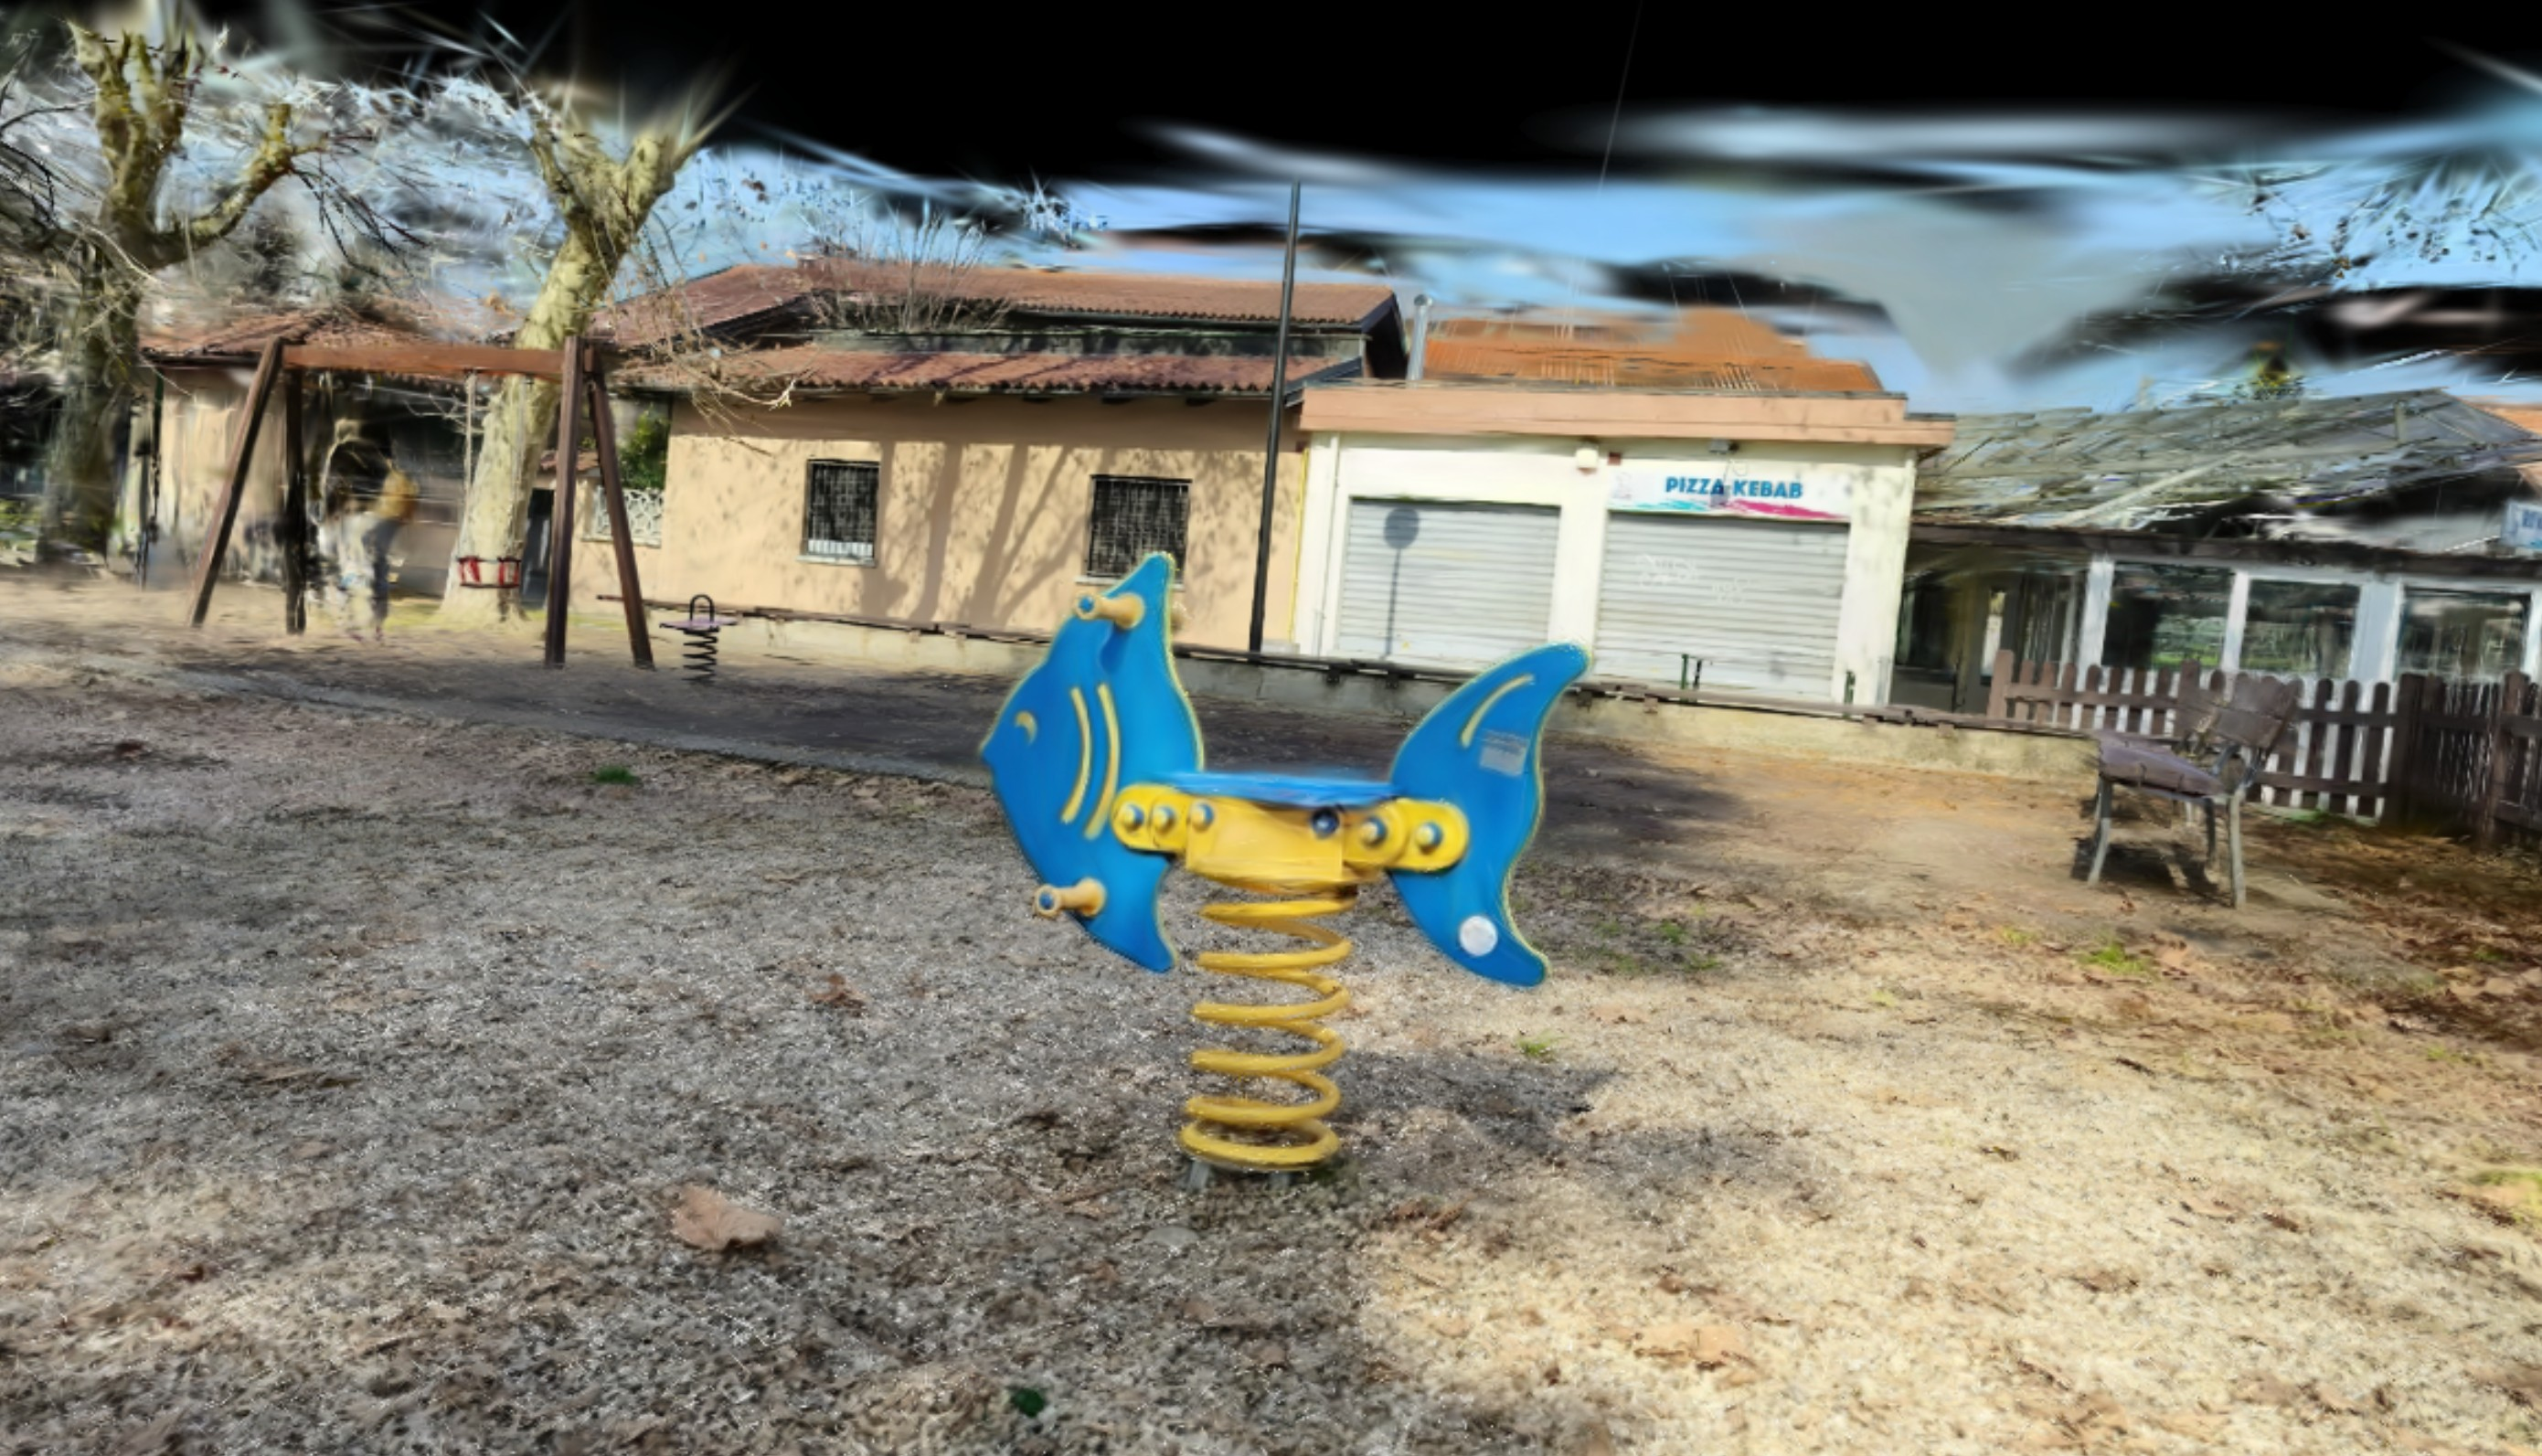
\includegraphics[width=0.32\textwidth,height=2.8cm,trim={80 40 80 40},clip]{images/benchmarks/spring_rider_inria_balanced_1.jpg}
	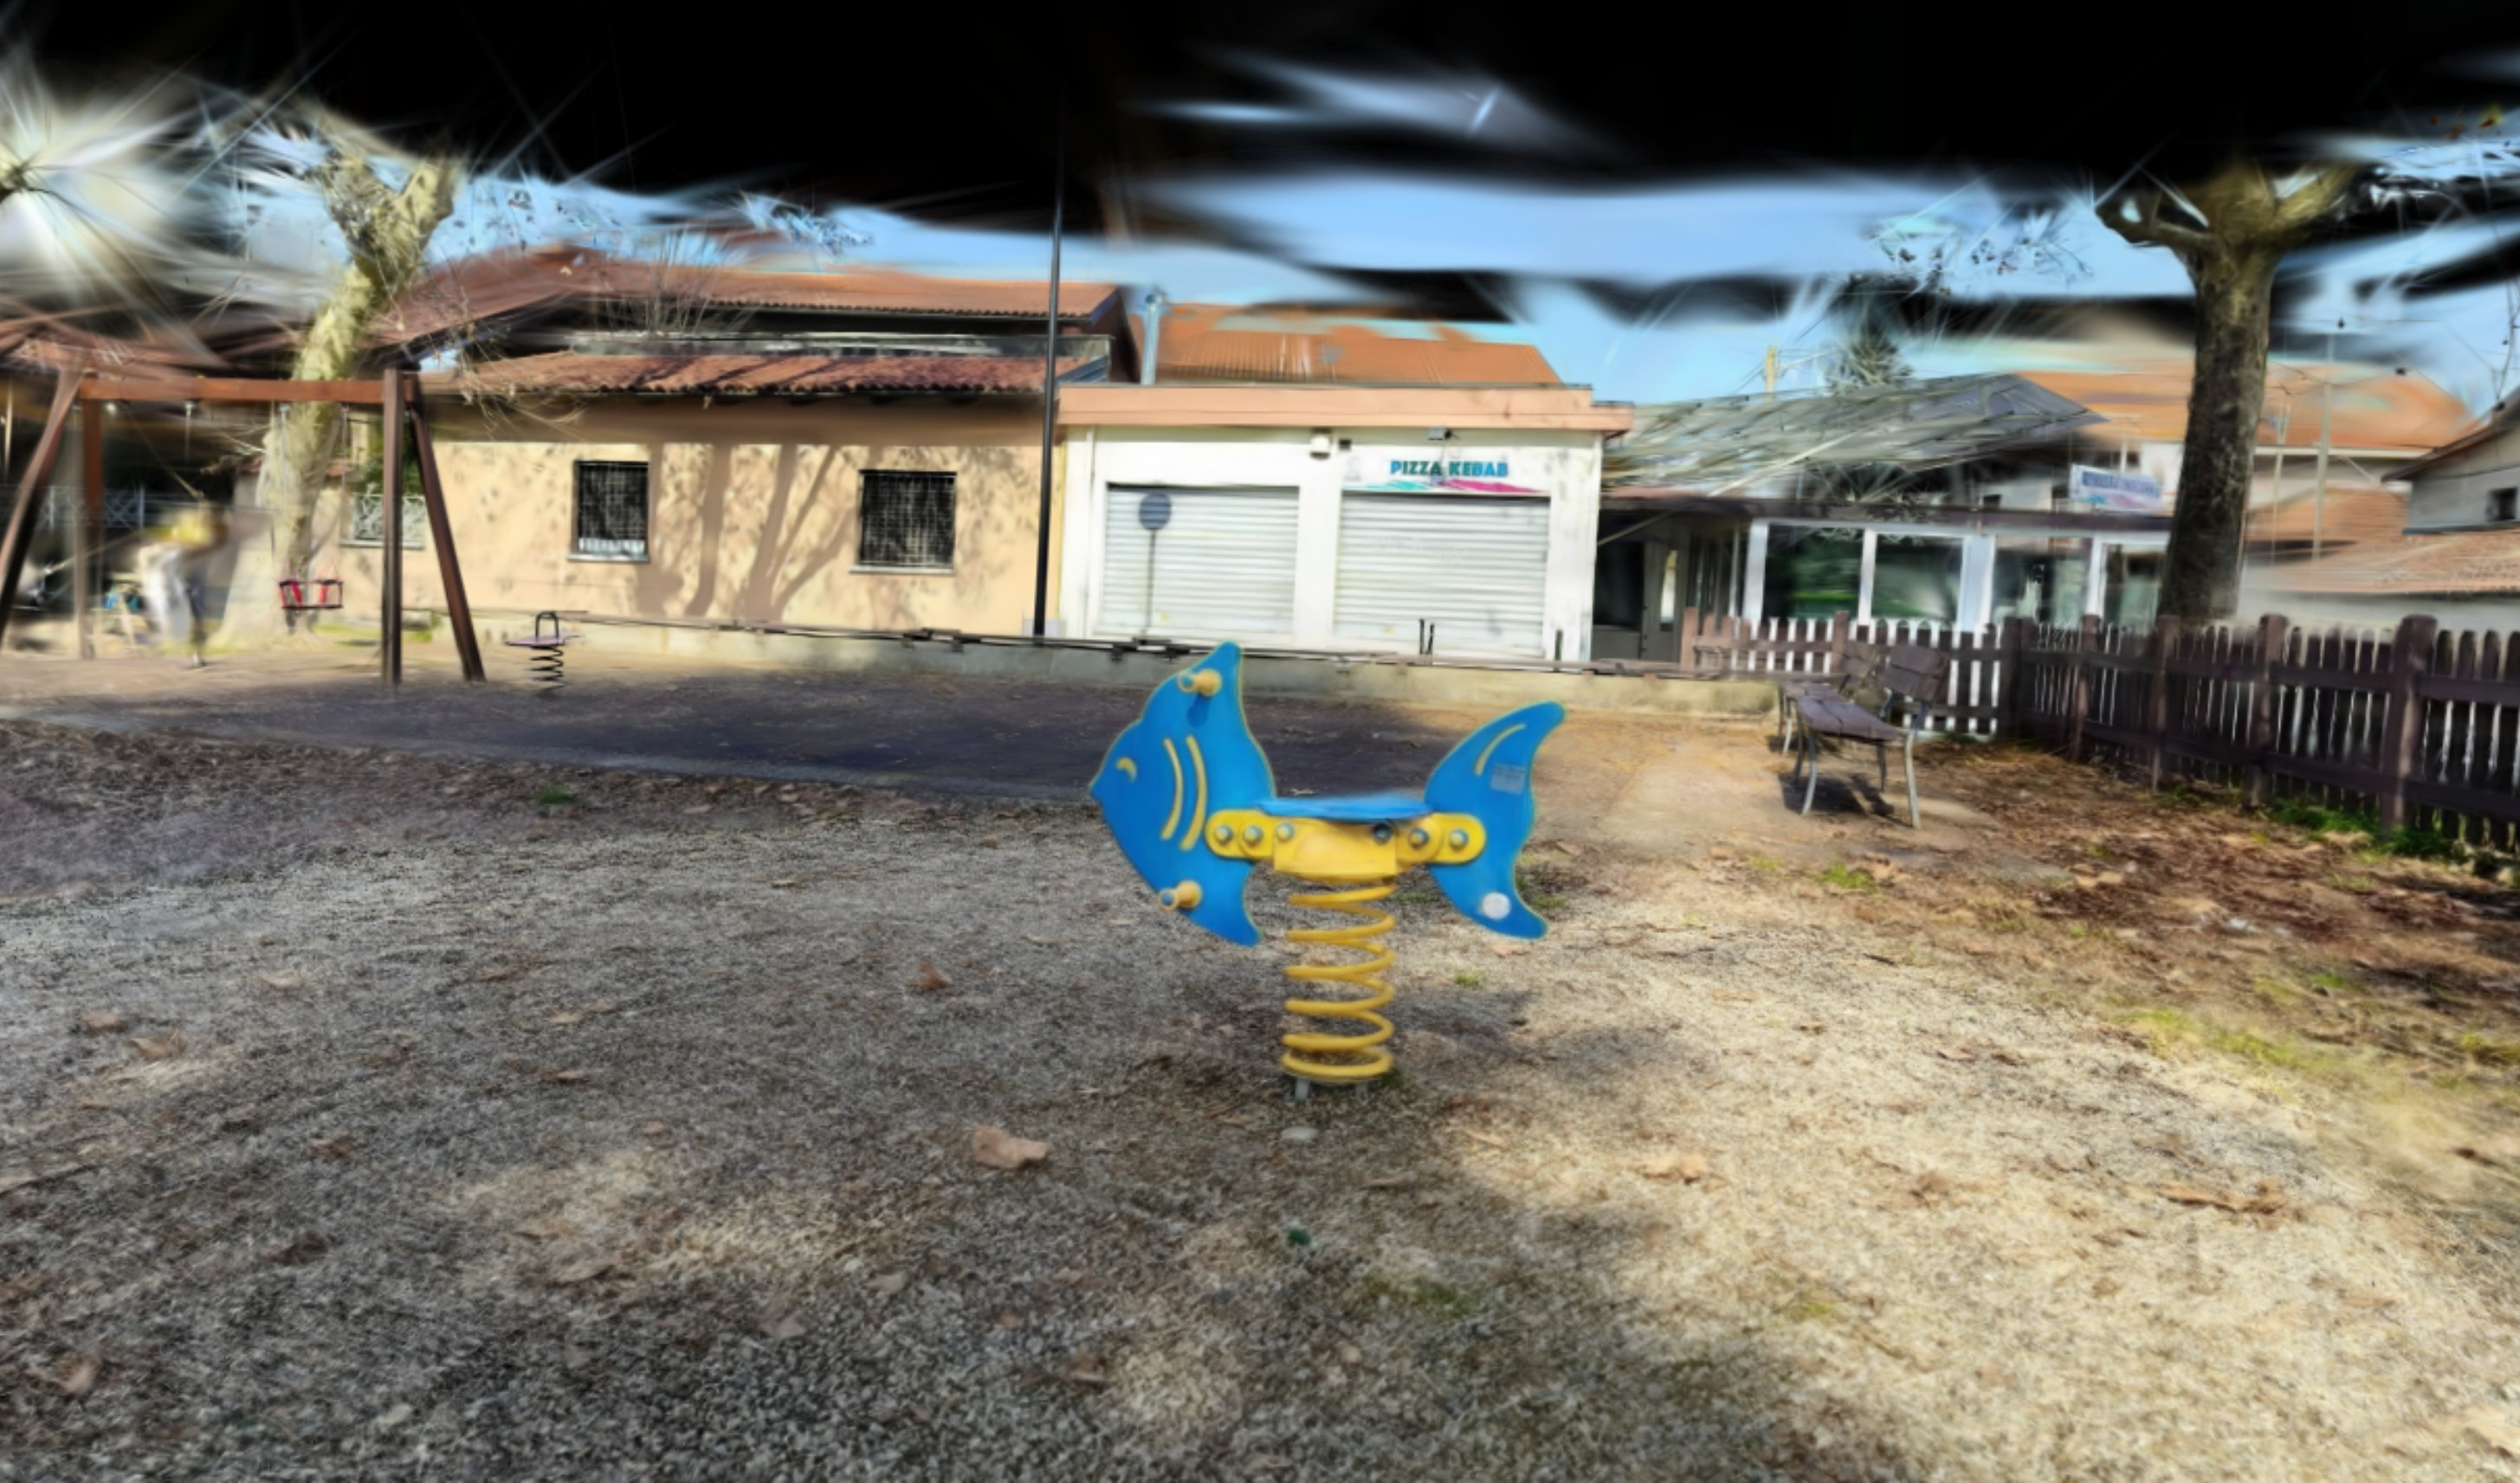
\includegraphics[width=0.32\textwidth,height=2.8cm,trim={80 40 80 40},clip]{images/benchmarks/spring_rider_mcmc_balanced_1.jpg}
	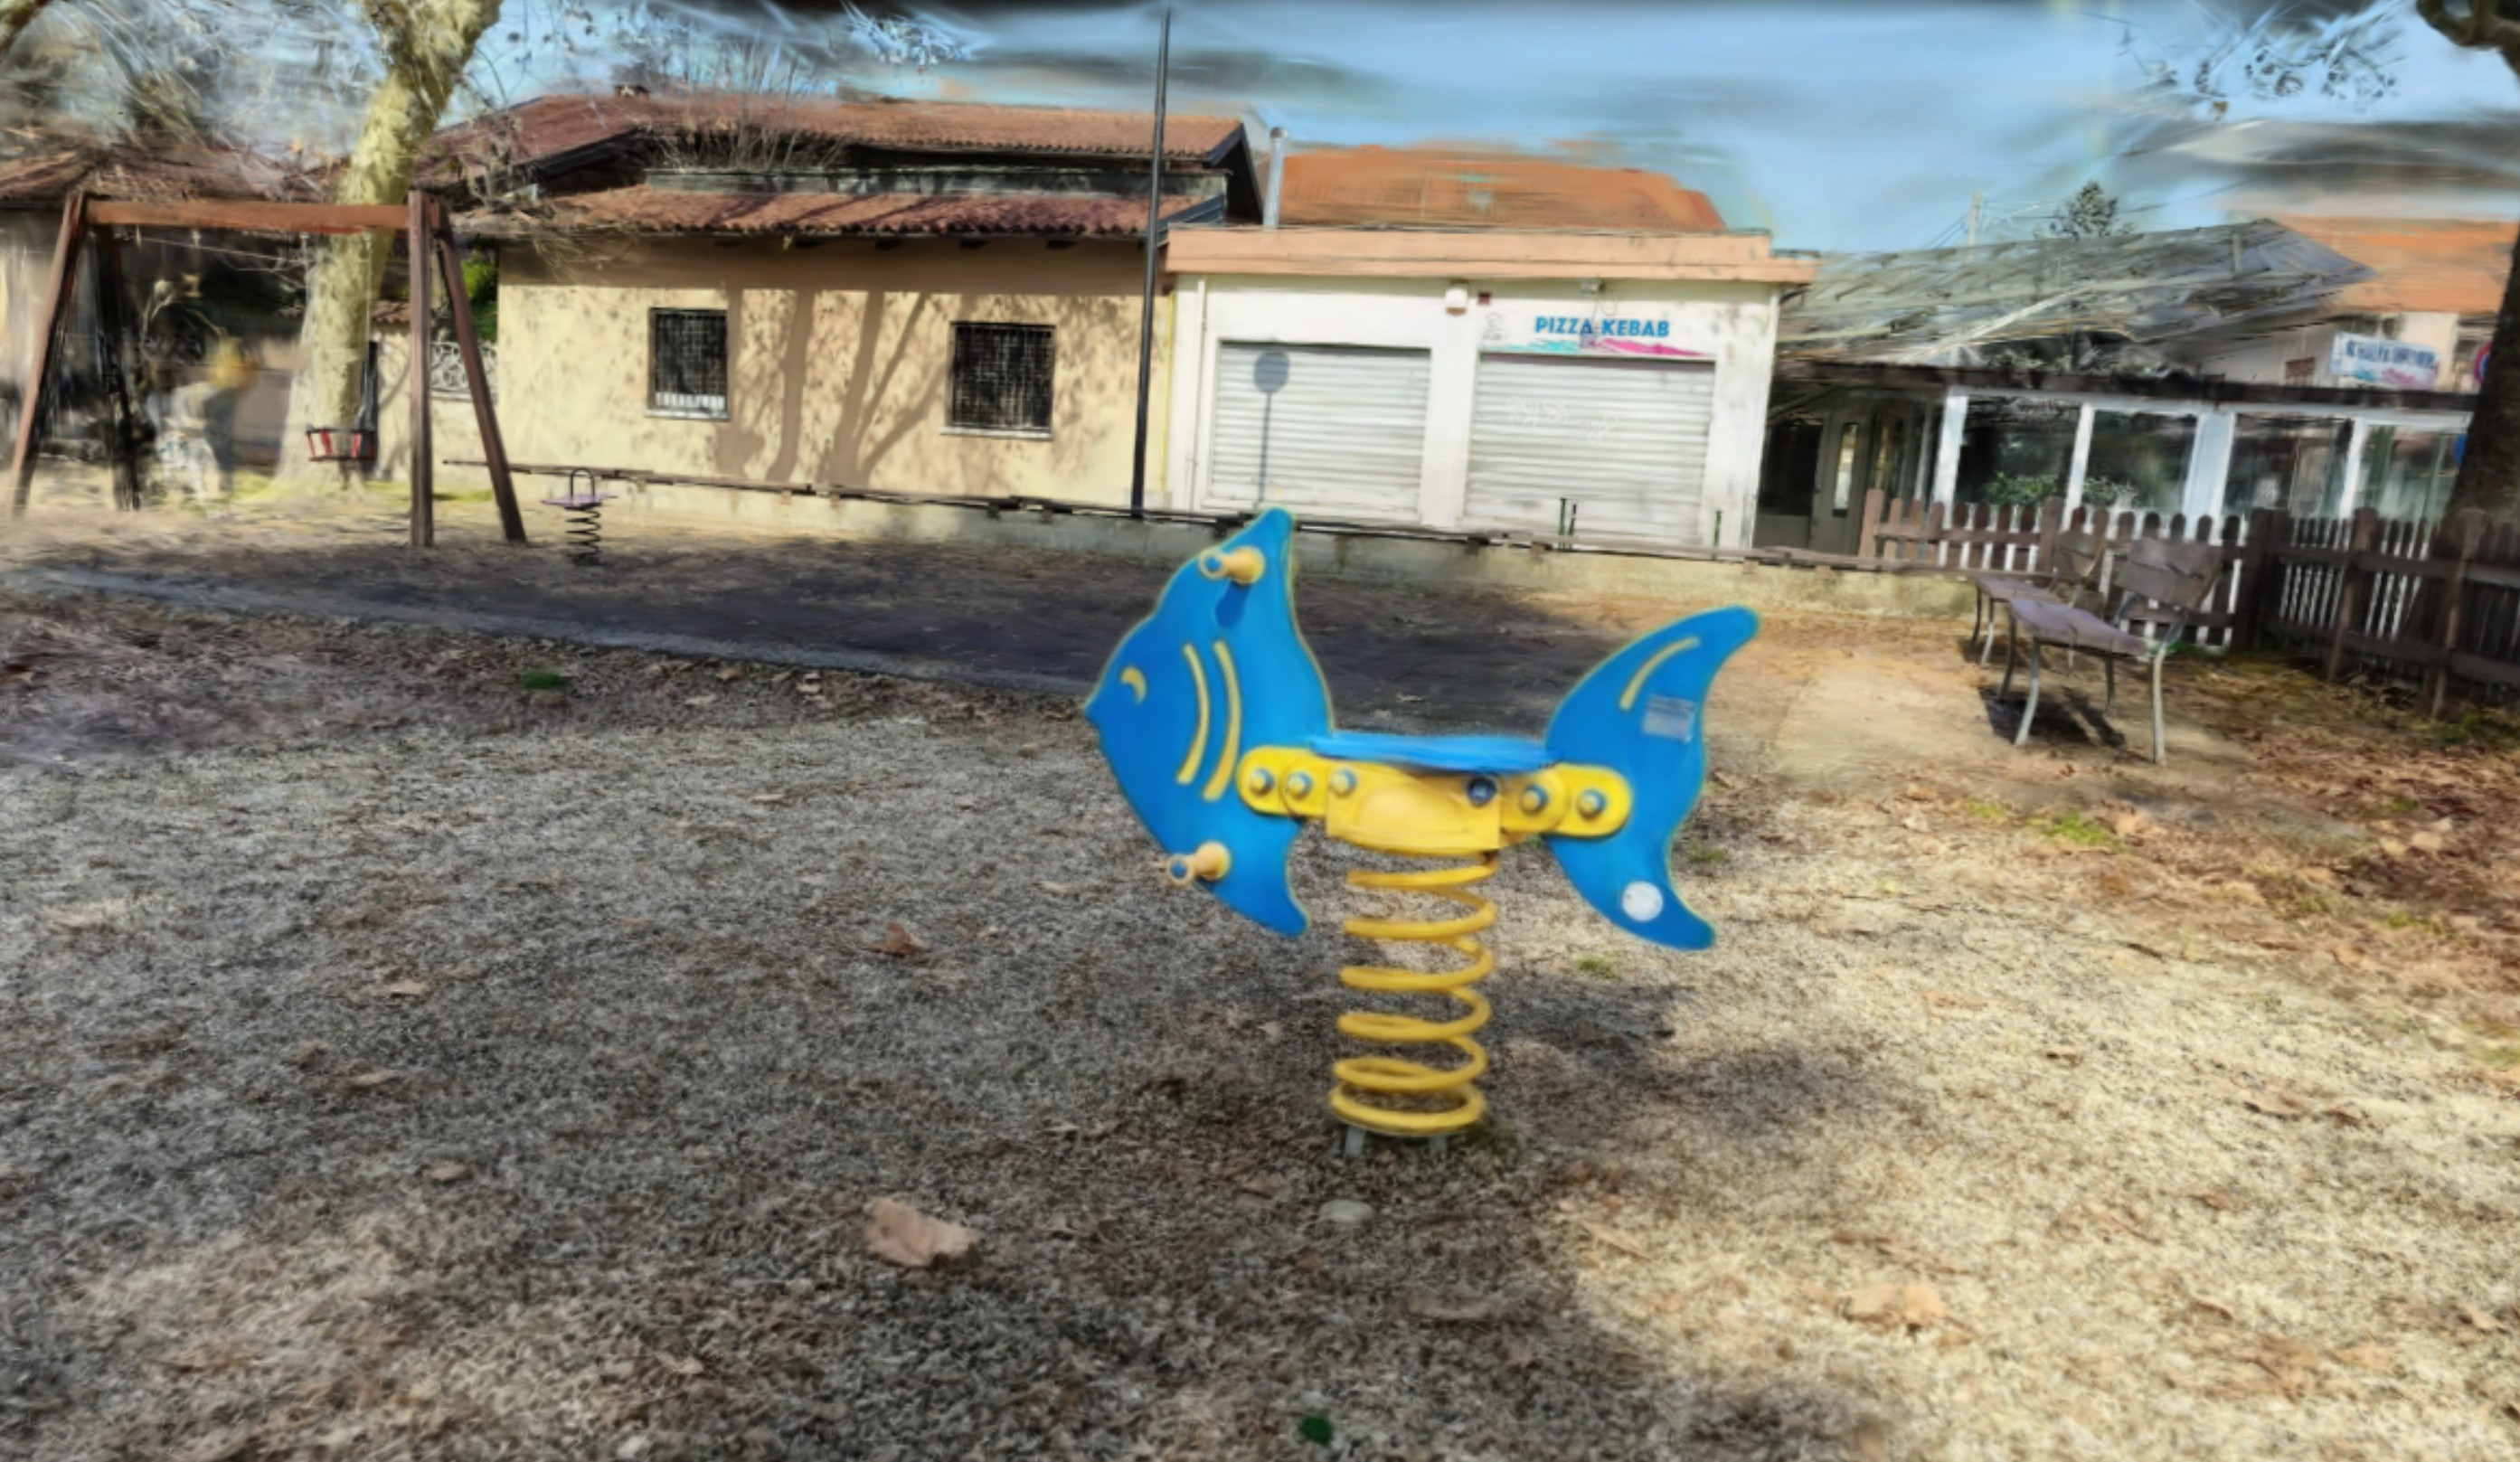
\includegraphics[width=0.32\textwidth,height=2.8cm,trim={80 40 80 40},clip]{images/benchmarks/spring_rider_taming_balanced_1.jpg}
	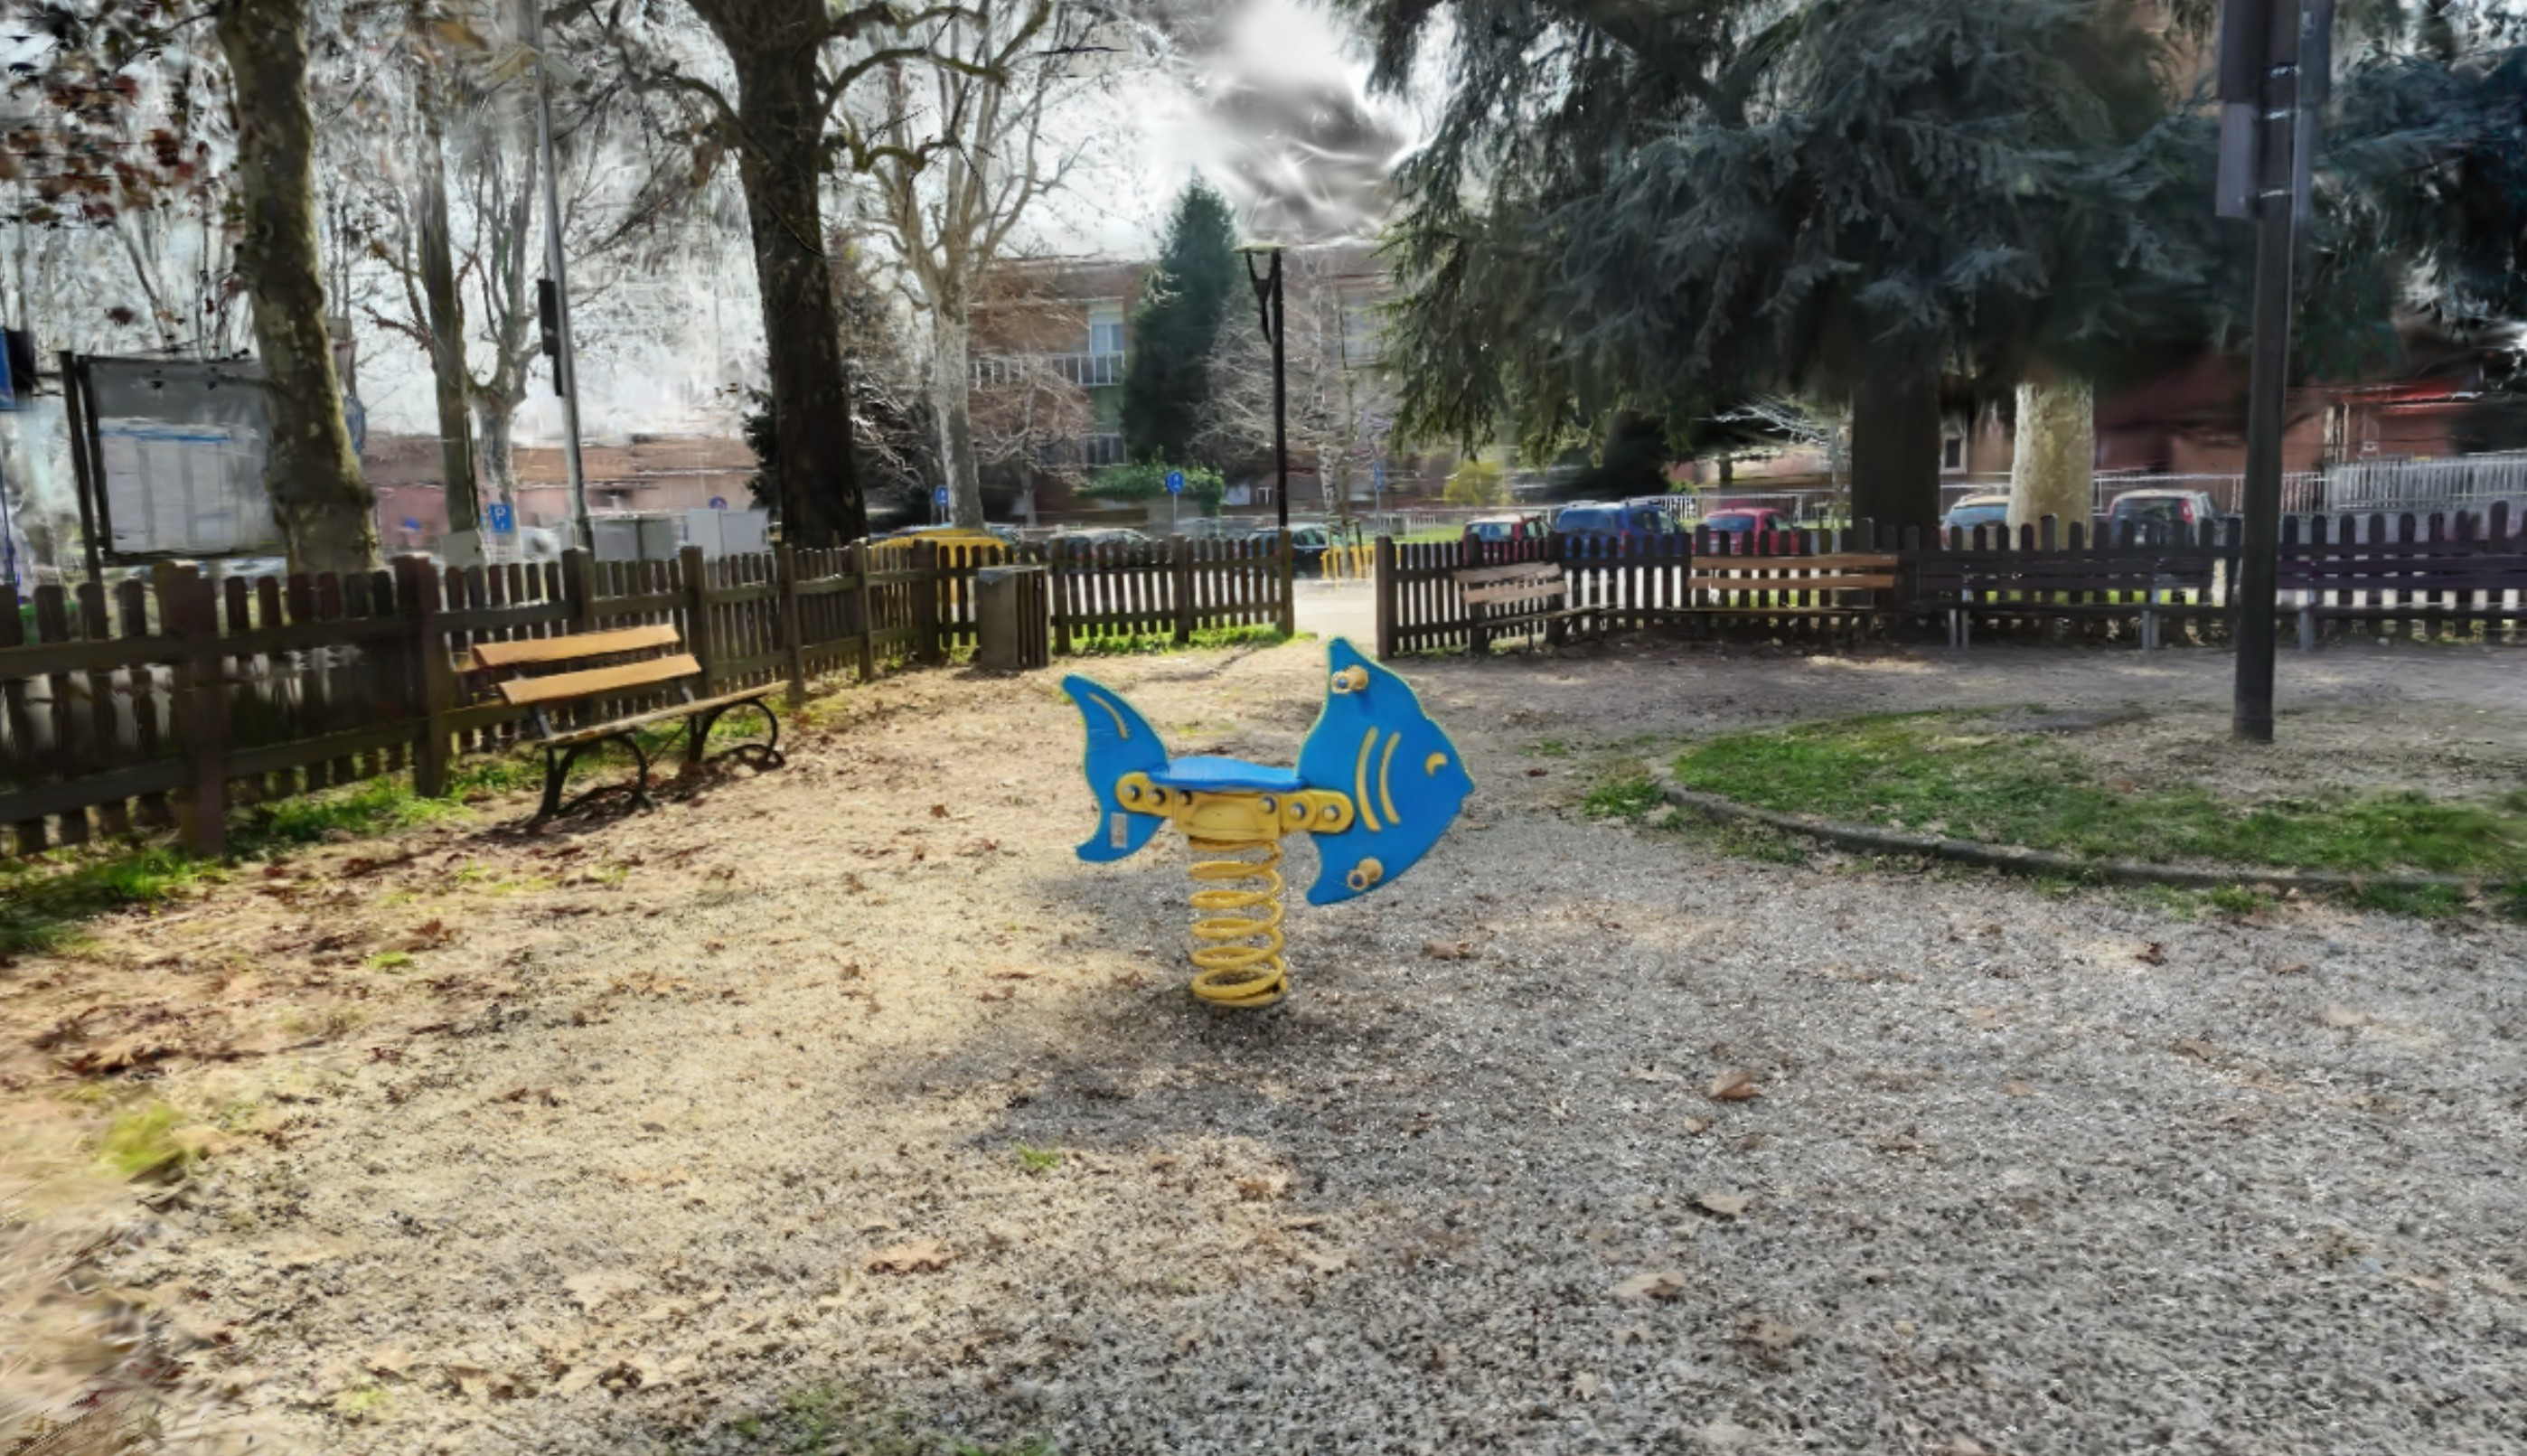
\includegraphics[width=0.32\textwidth,height=2.8cm,trim={80 40 80 40},clip]{images/benchmarks/spring_rider_inria_balanced_2.jpg}
	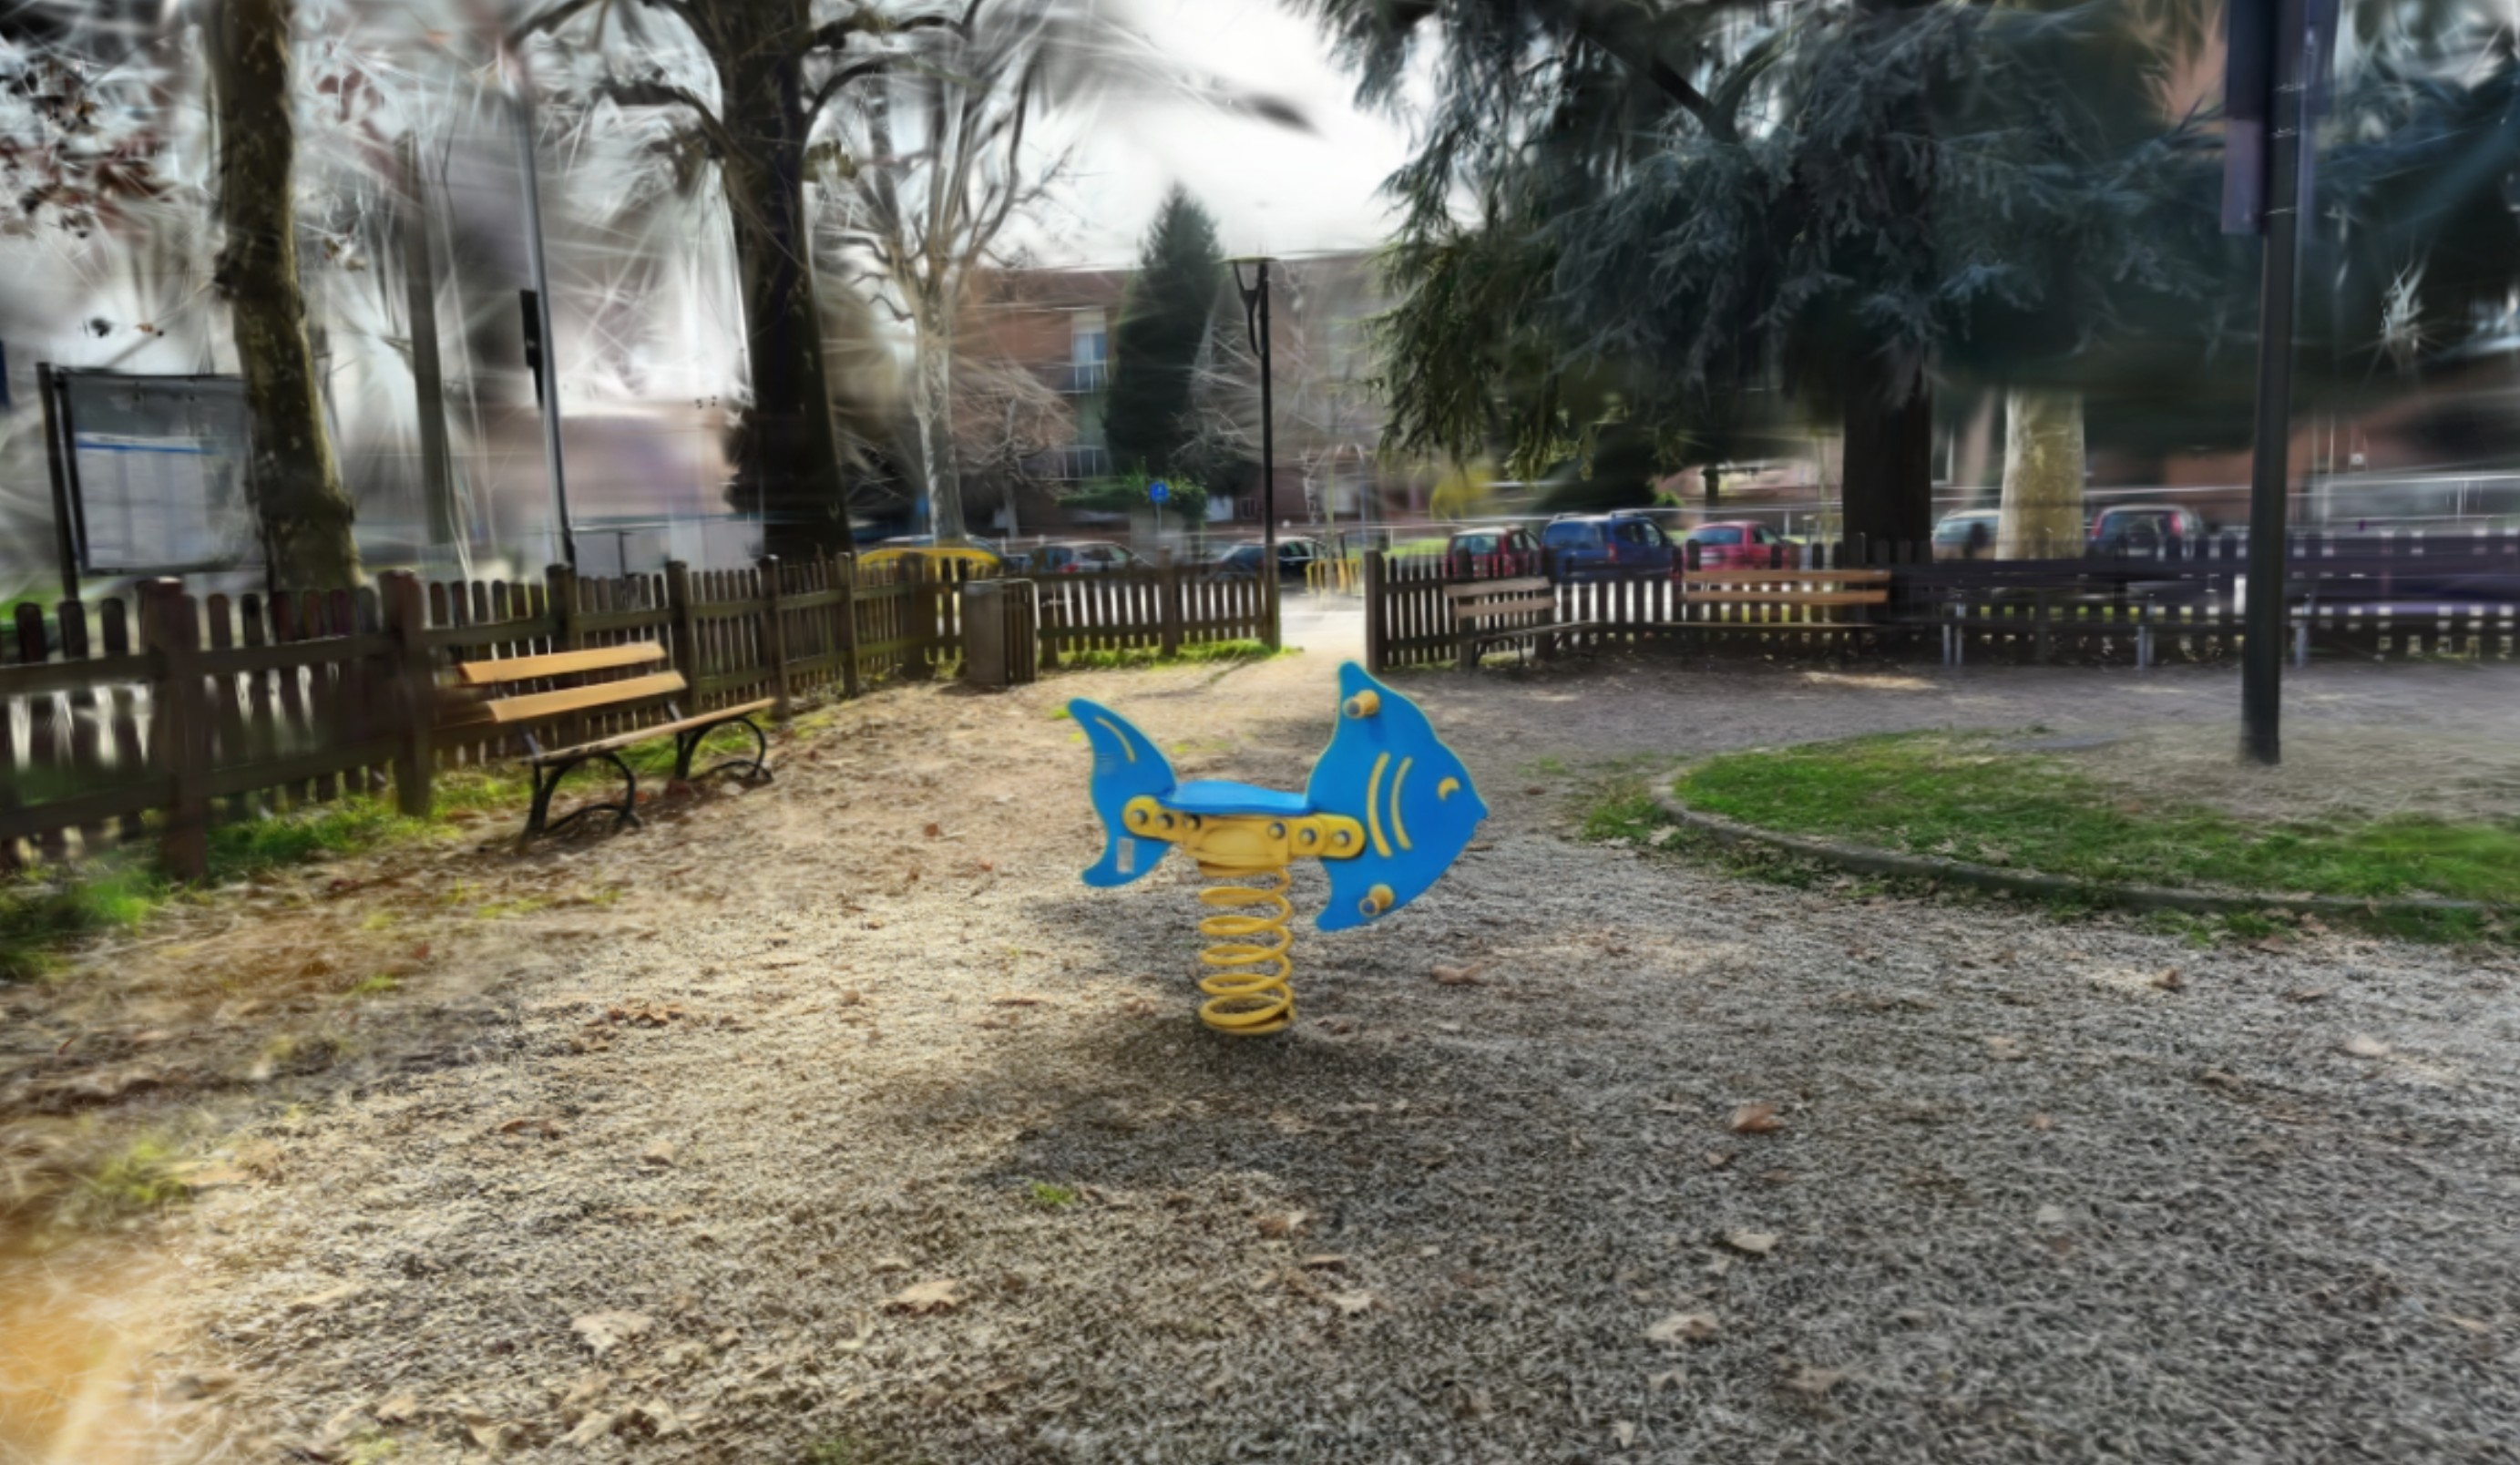
\includegraphics[width=0.32\textwidth,height=2.8cm,trim={80 40 80 40},clip]{images/benchmarks/spring_rider_mcmc_balanced_2.jpg}
	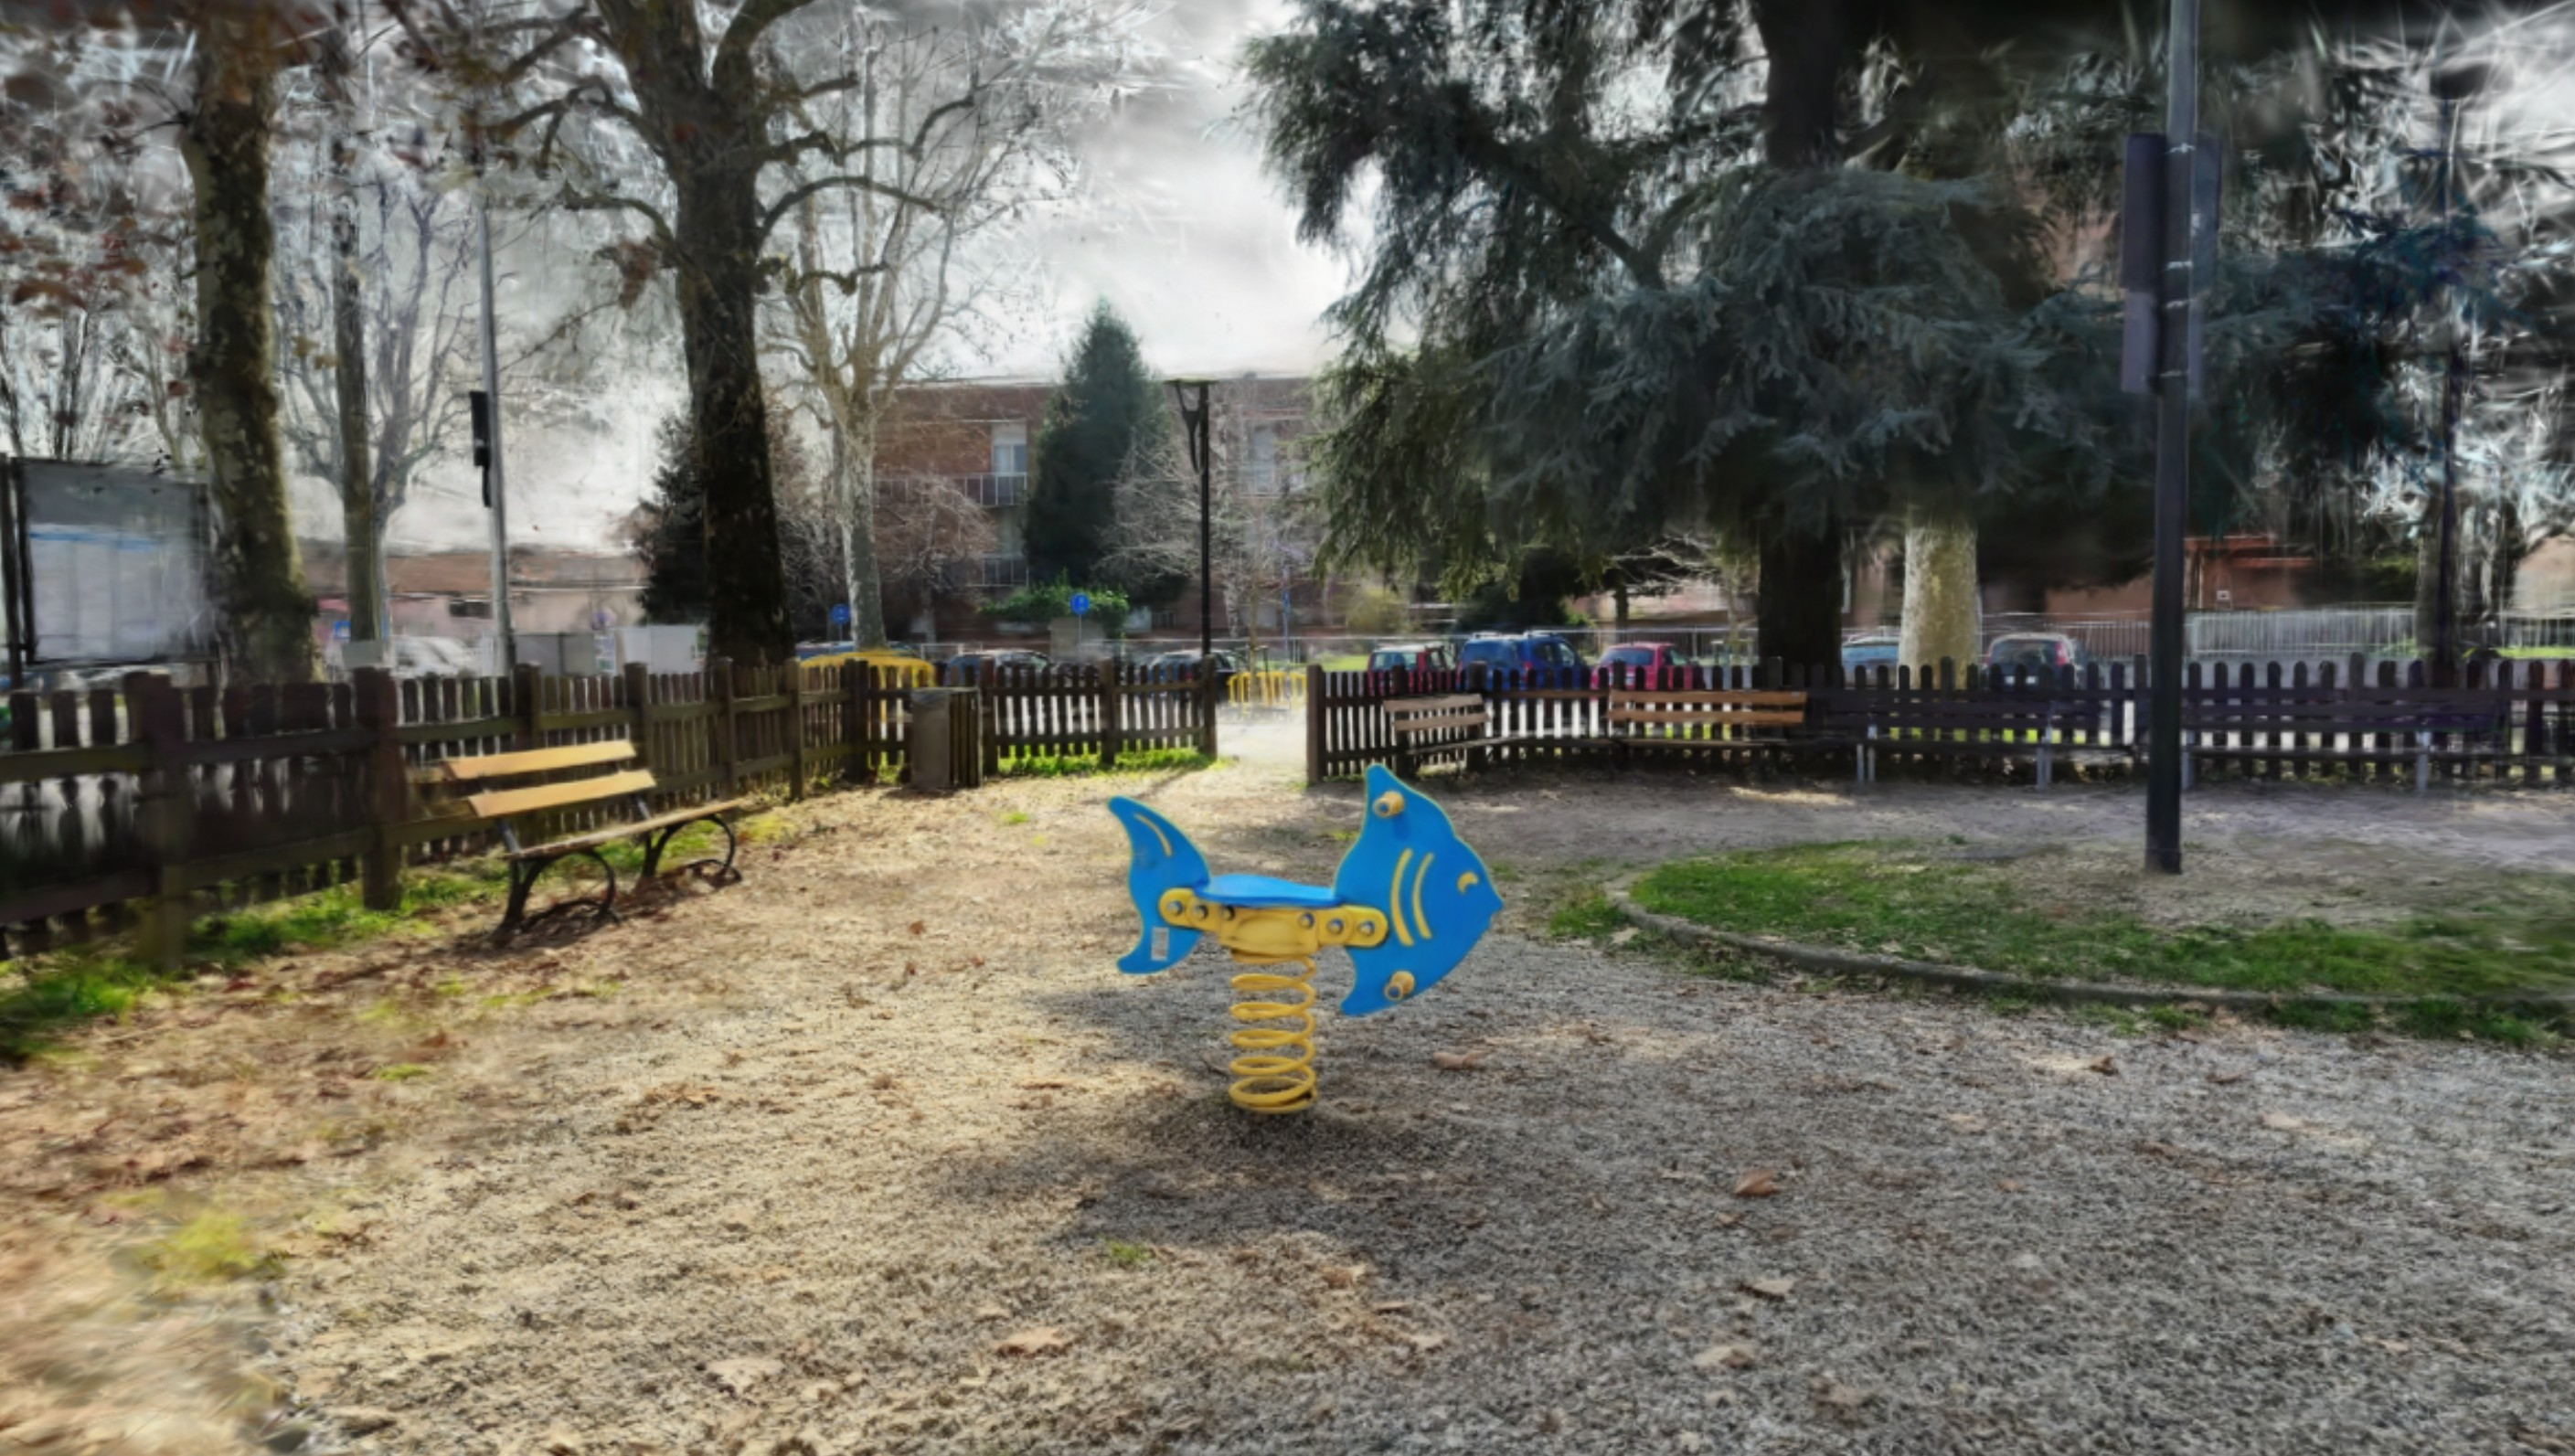
\includegraphics[width=0.32\textwidth,height=2.8cm,trim={80 40 80 40},clip]{images/benchmarks/spring_rider_taming_balanced_2.jpg}
	\caption{Confronto visivo Spring Rider (crop centrale) -- INRIA / MCMC / Taming}
	\label{fig:spring_rider_comparison}
\end{figure}


\begin{figure}[ht]
	\centering
	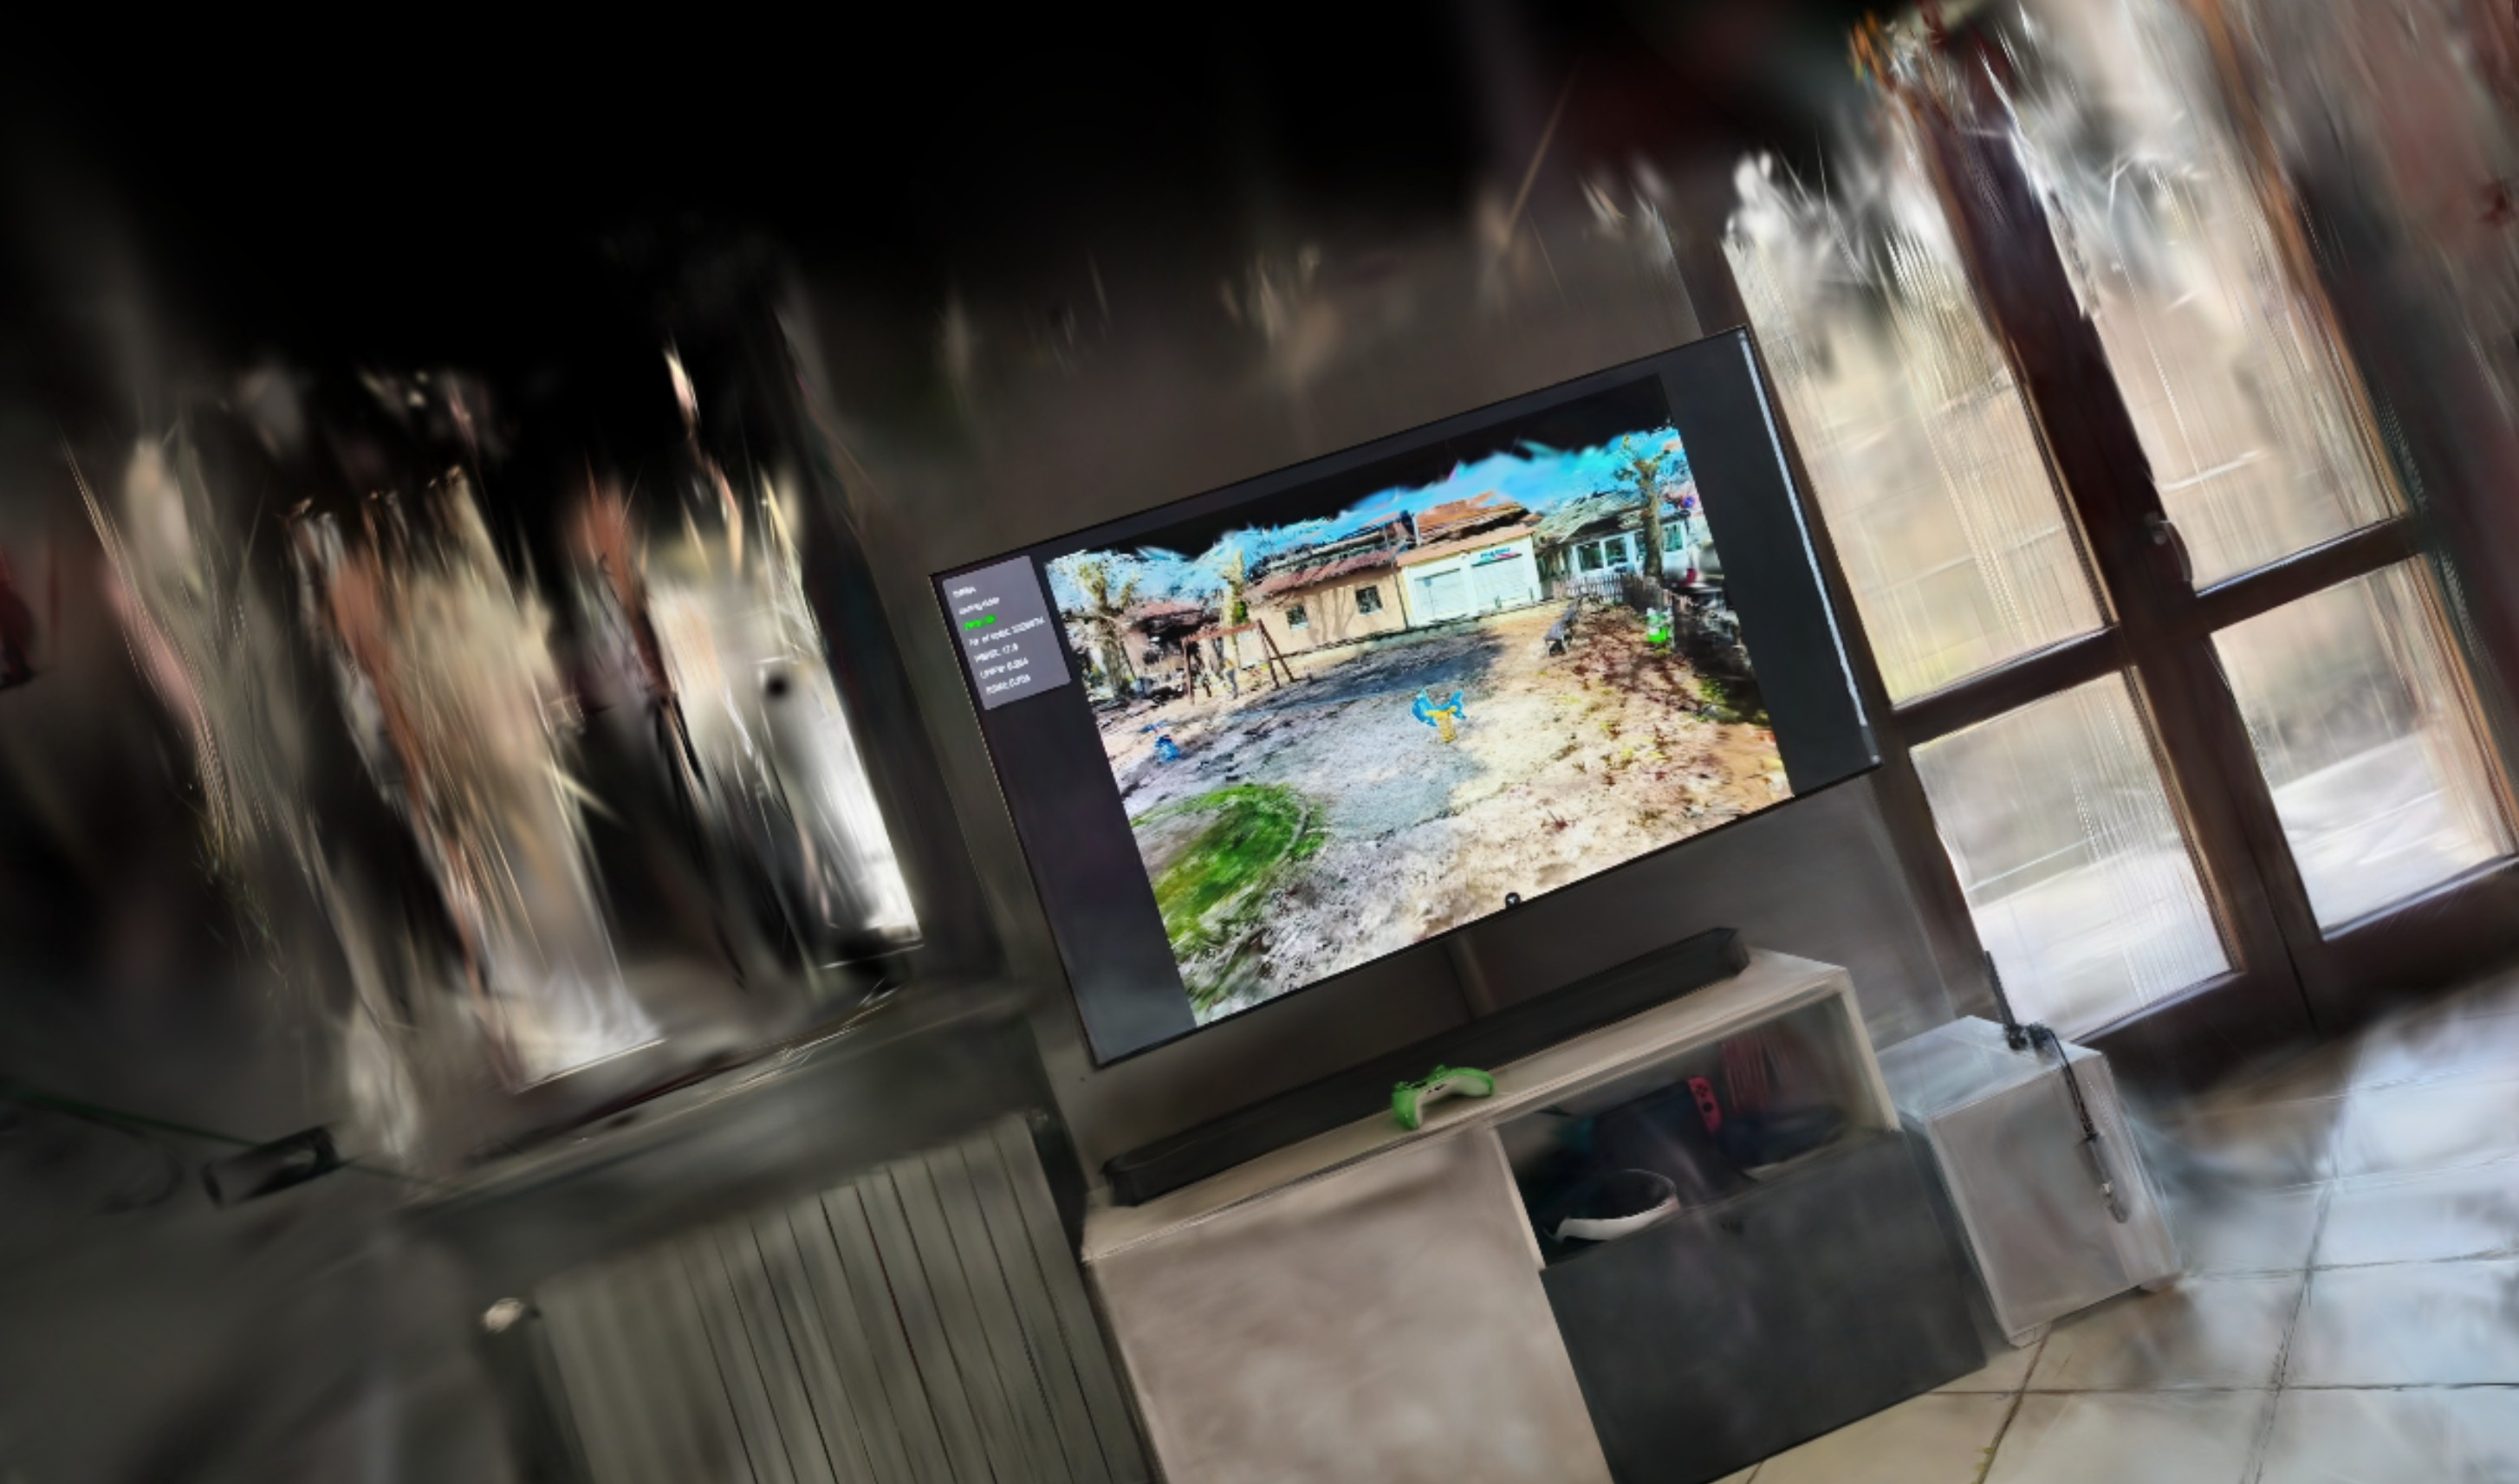
\includegraphics[width=0.32\textwidth,height=2.8cm,trim={80 40 80 40},clip]{images/benchmarks/my_workstation_inria_balanced_1.jpg}
	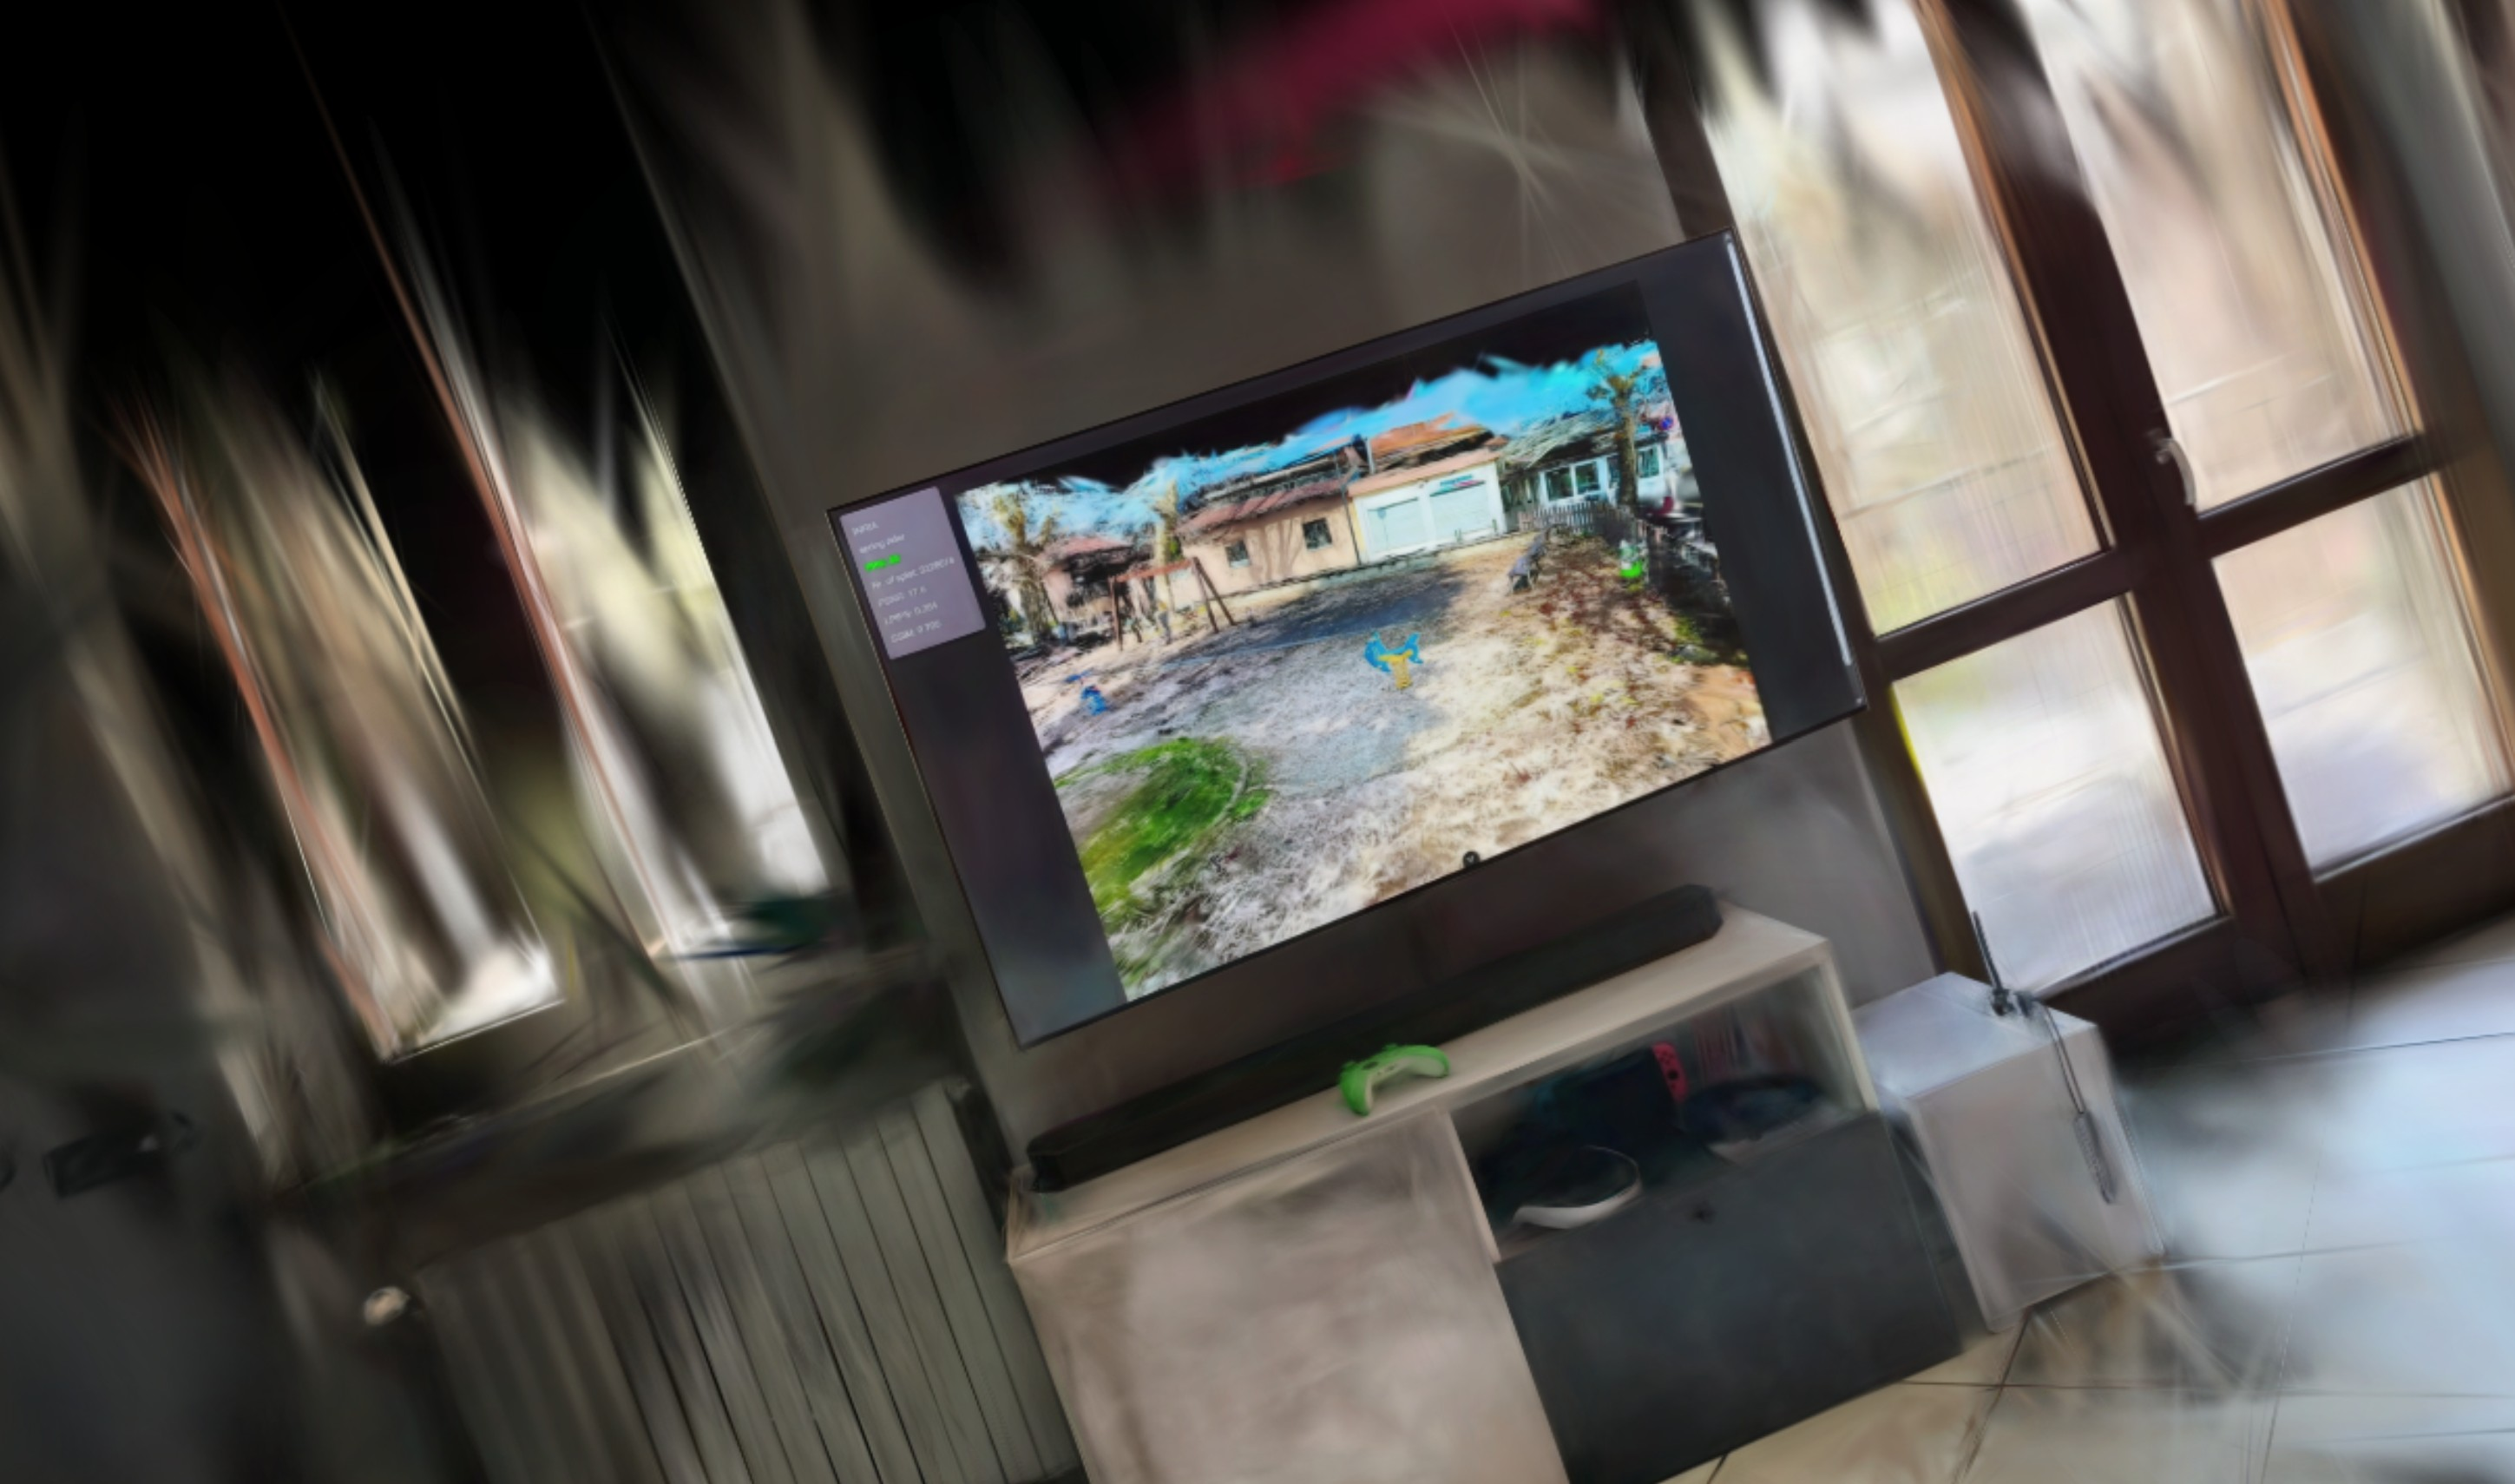
\includegraphics[width=0.32\textwidth,height=2.8cm,trim={80 40 80 40},clip]{images/benchmarks/my_workstation_mcmc_balanced_1.jpg}
	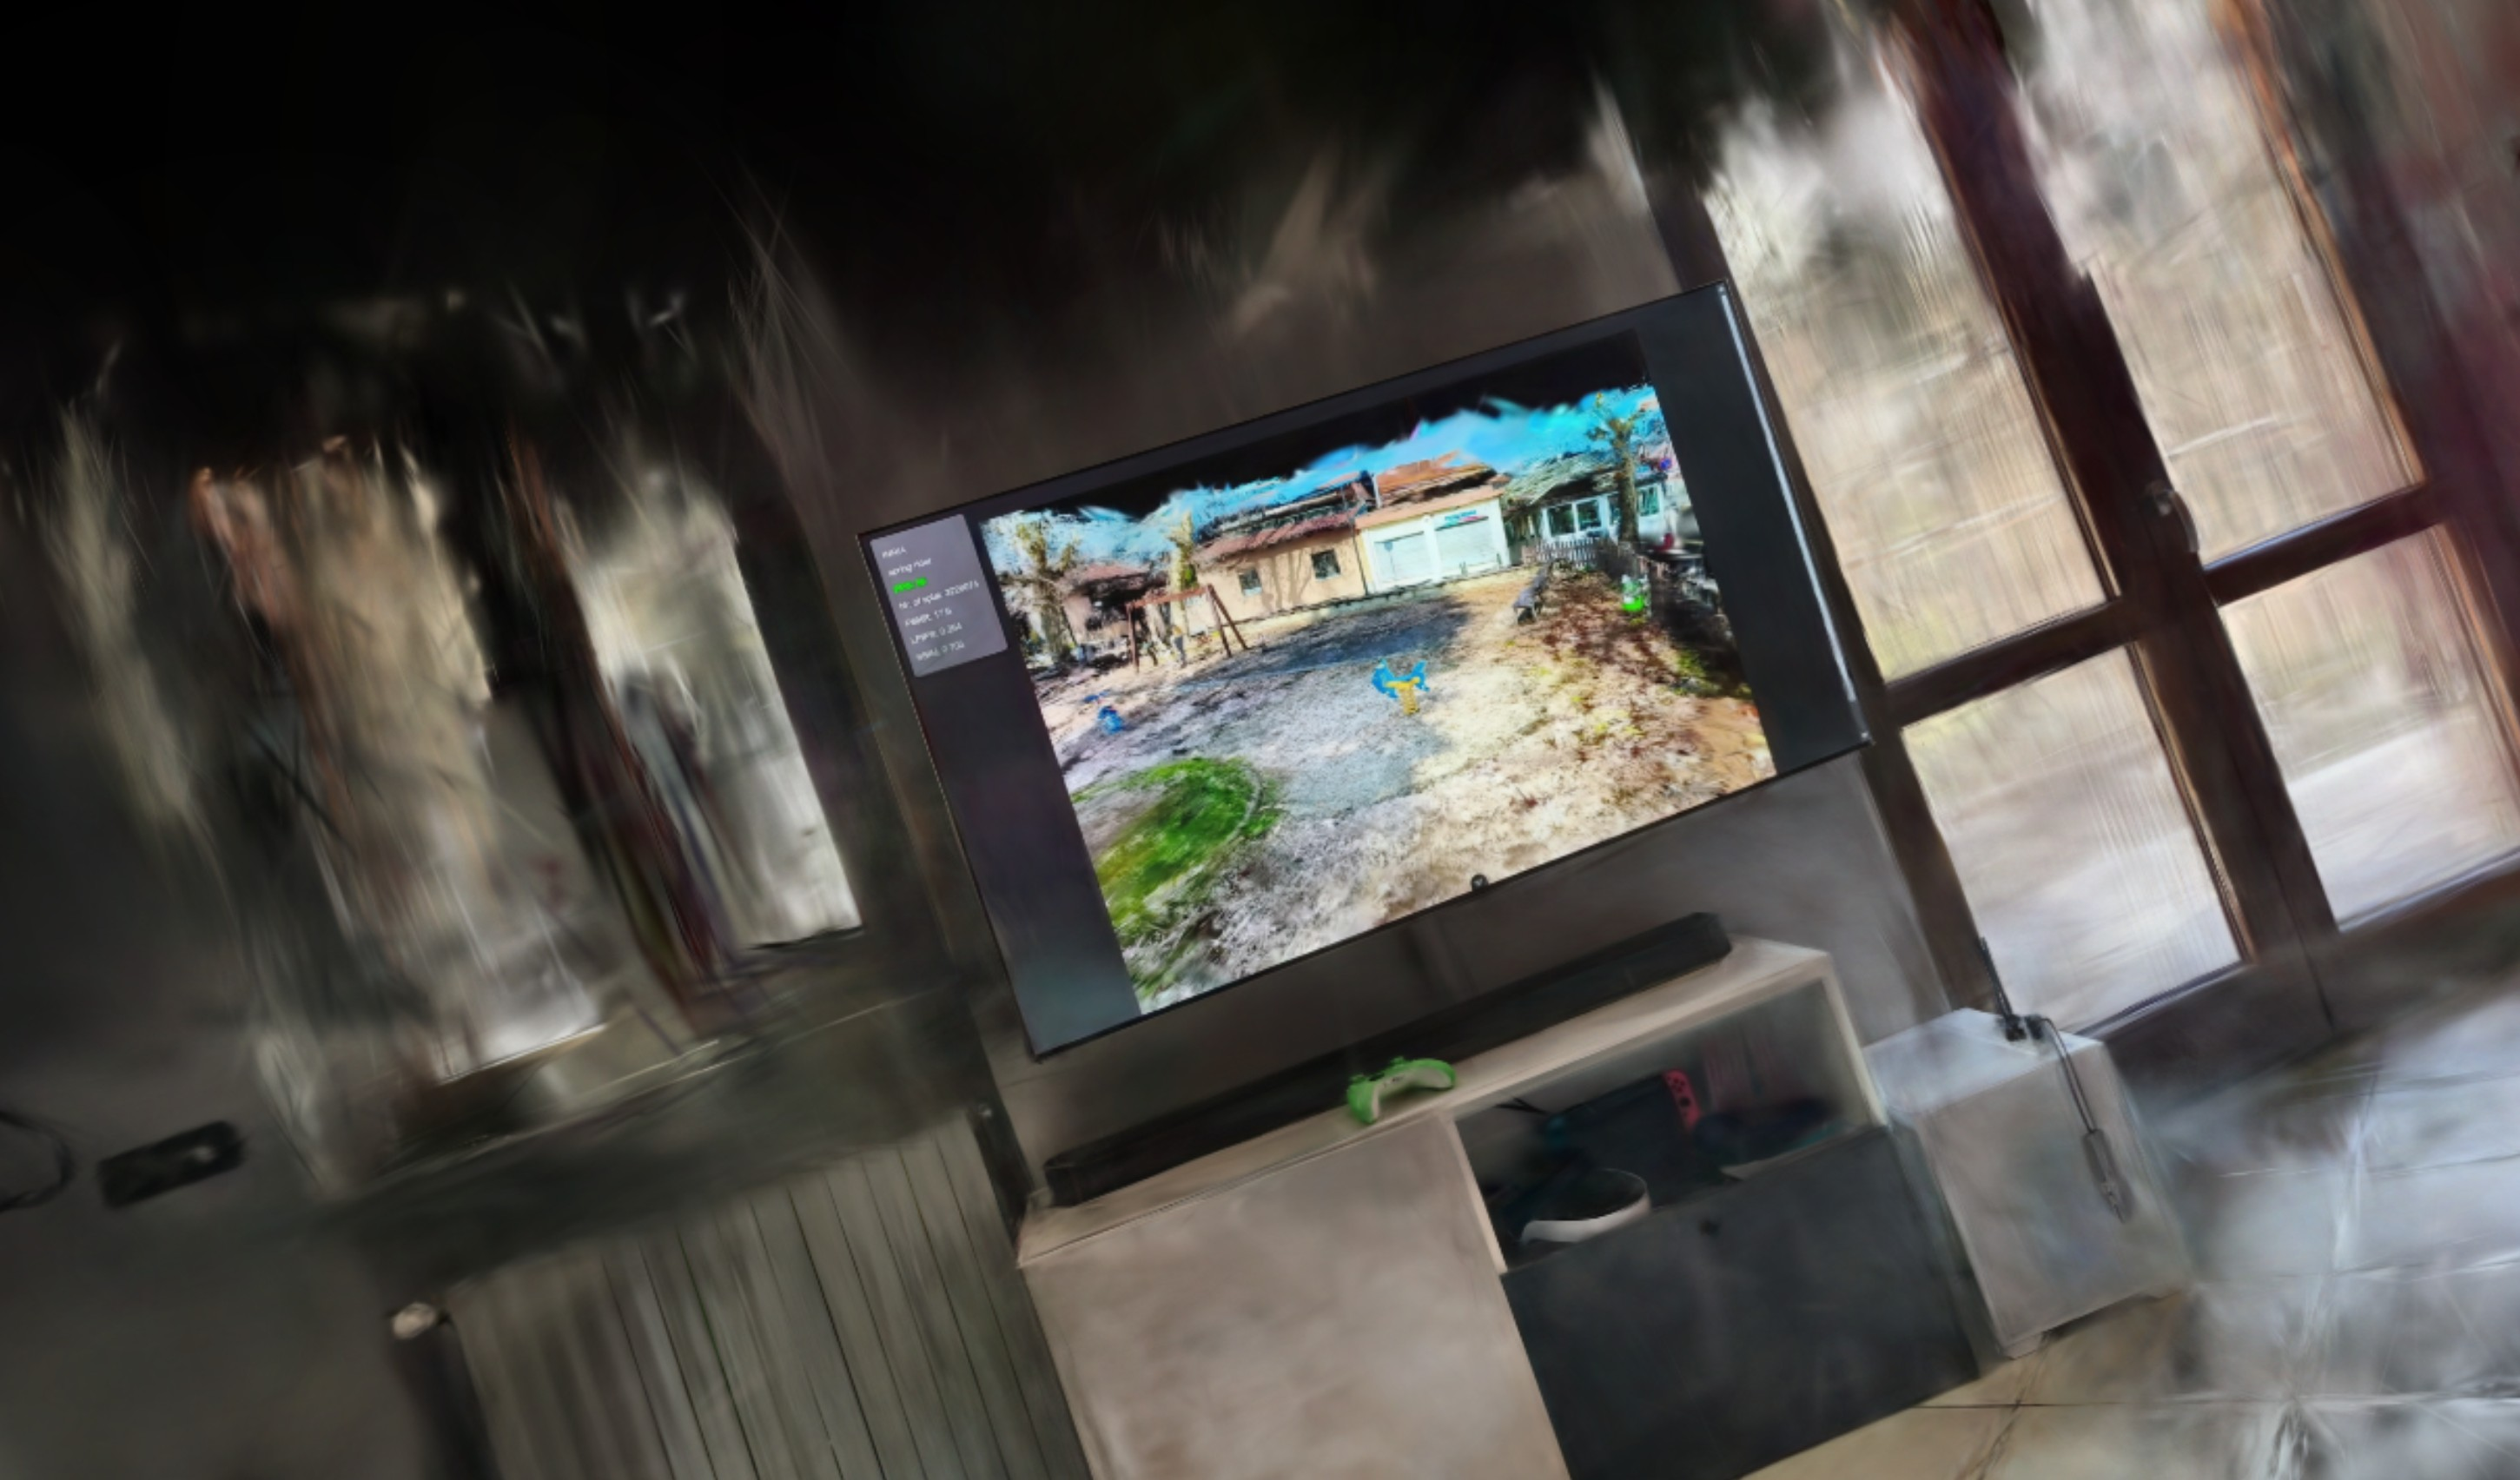
\includegraphics[width=0.32\textwidth,height=2.8cm,trim={80 40 80 40},clip]{images/benchmarks/my_workstation_taming_balanced_1.jpg}
		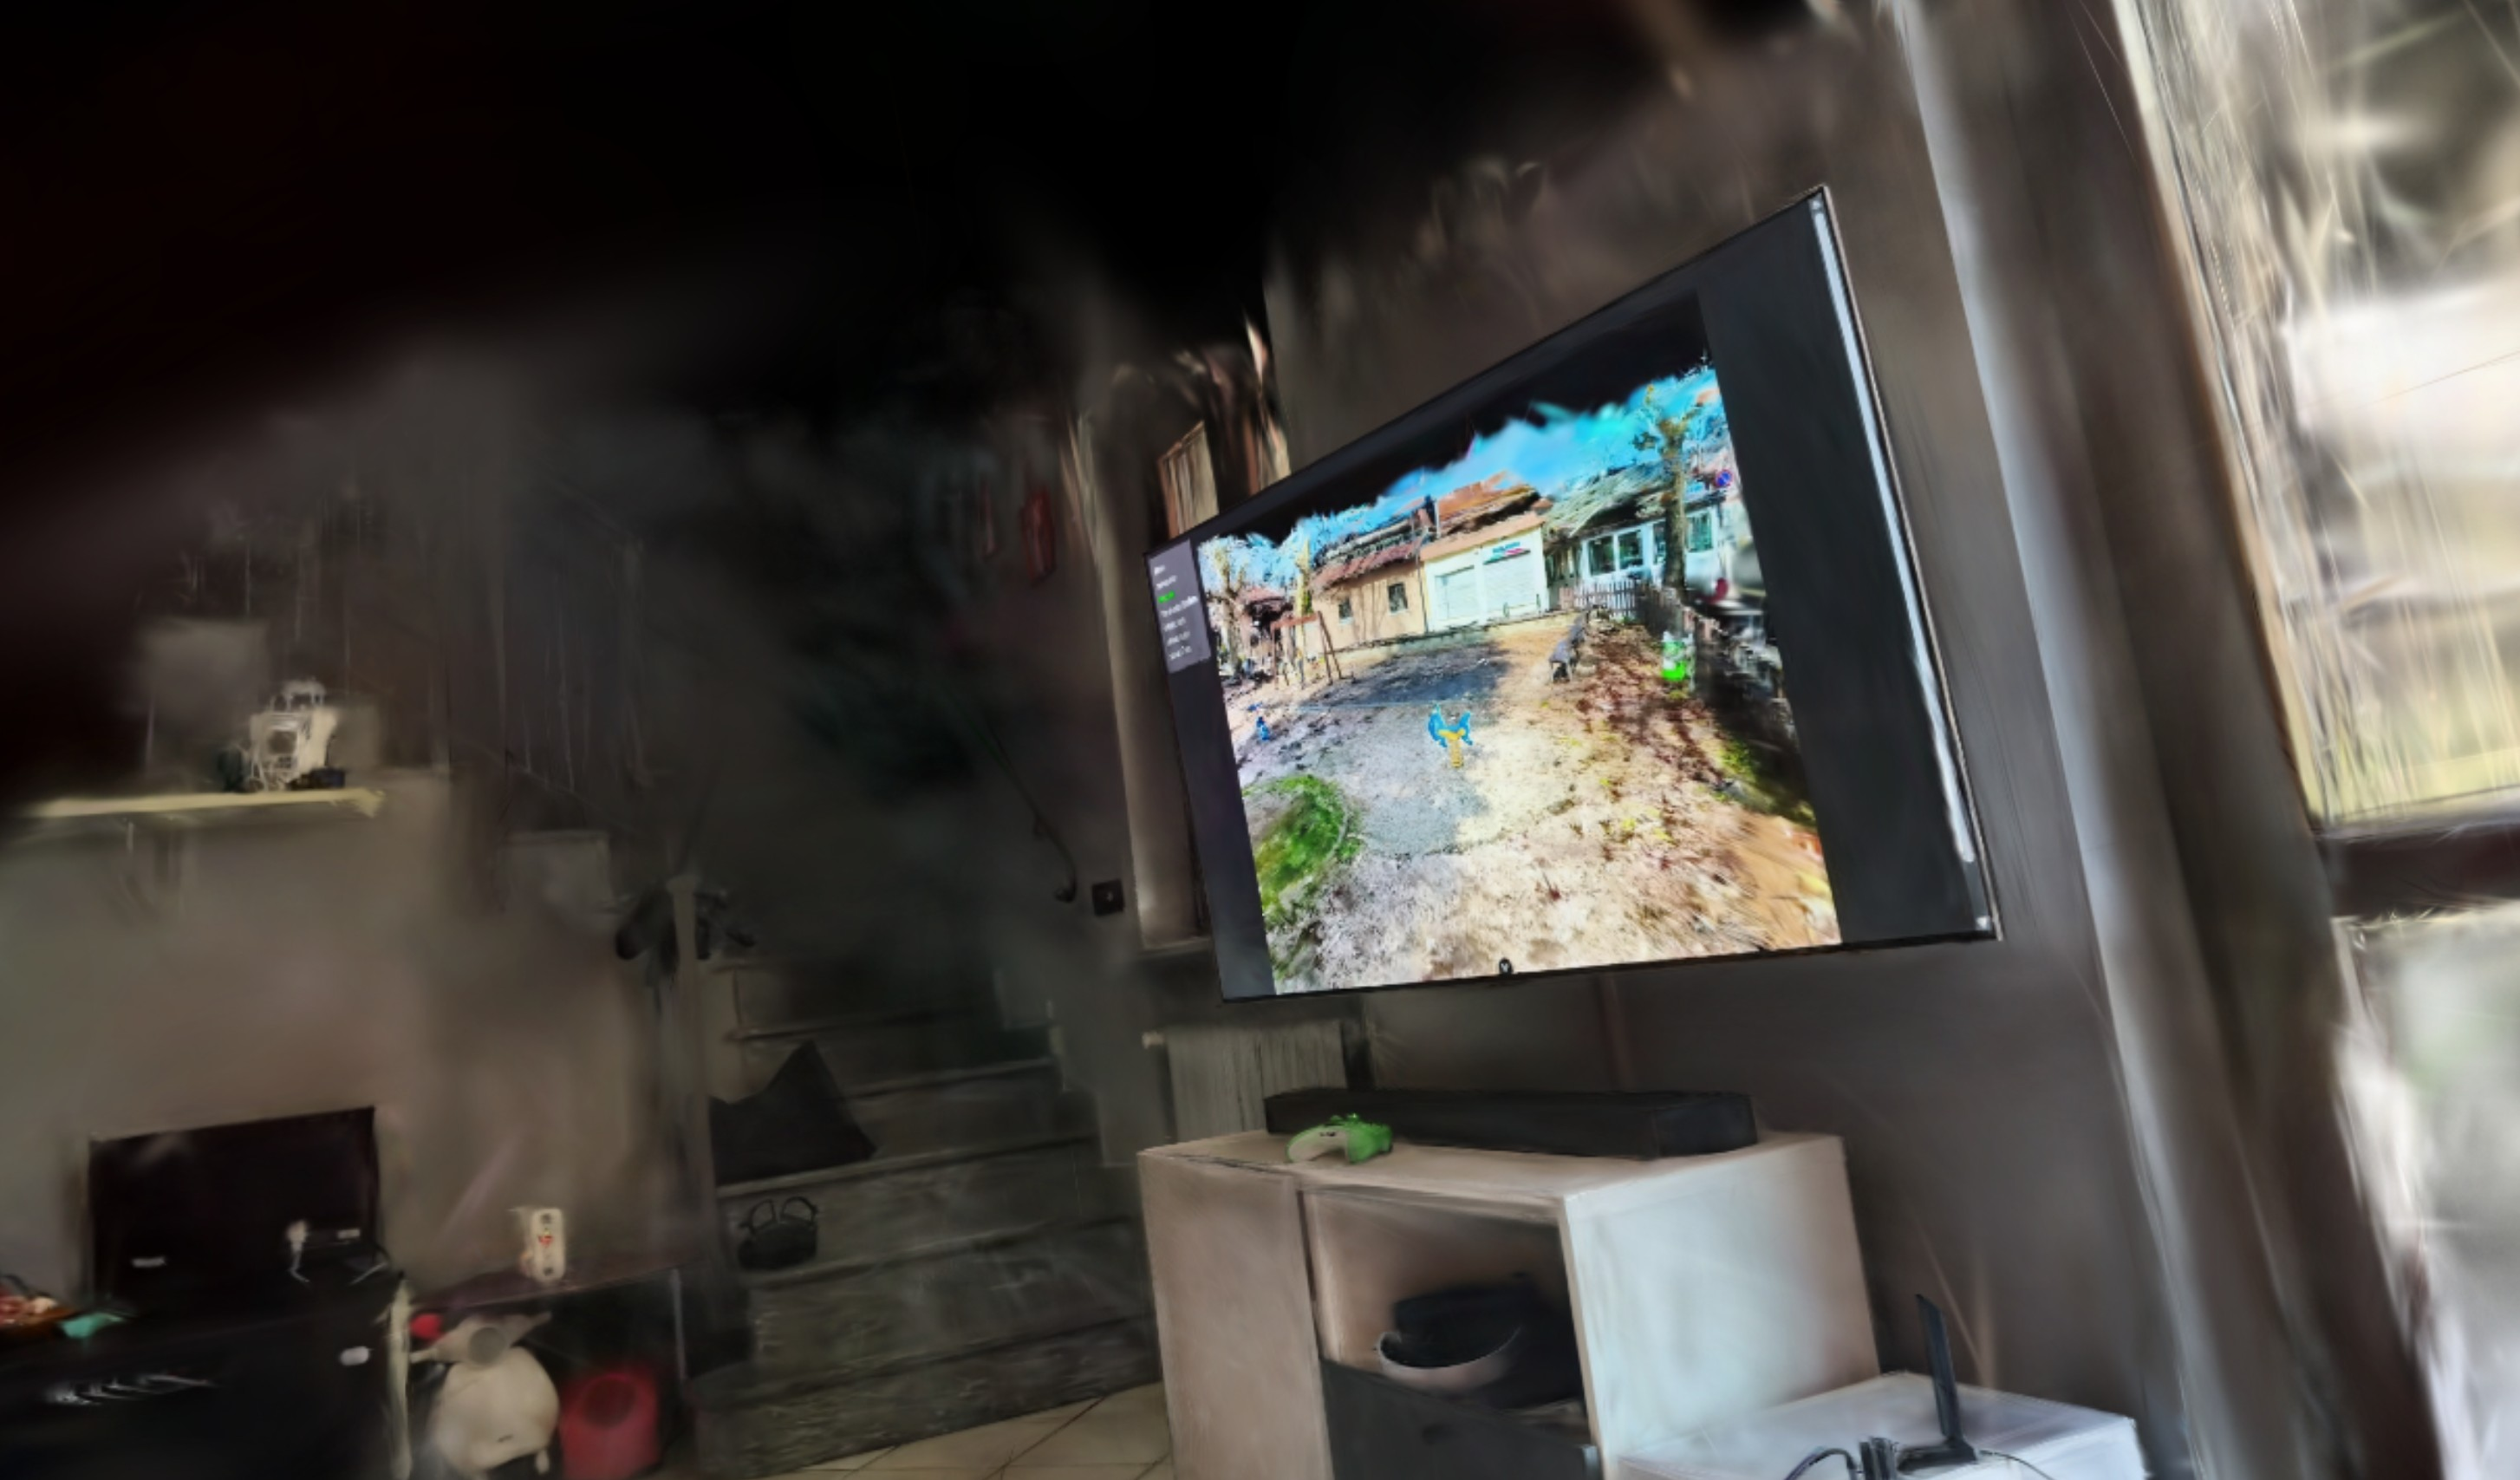
\includegraphics[width=0.32\textwidth,height=2.8cm,trim={80 40 80 40},clip]{images/benchmarks/my_workstation_inria_balanced_2.jpg}
	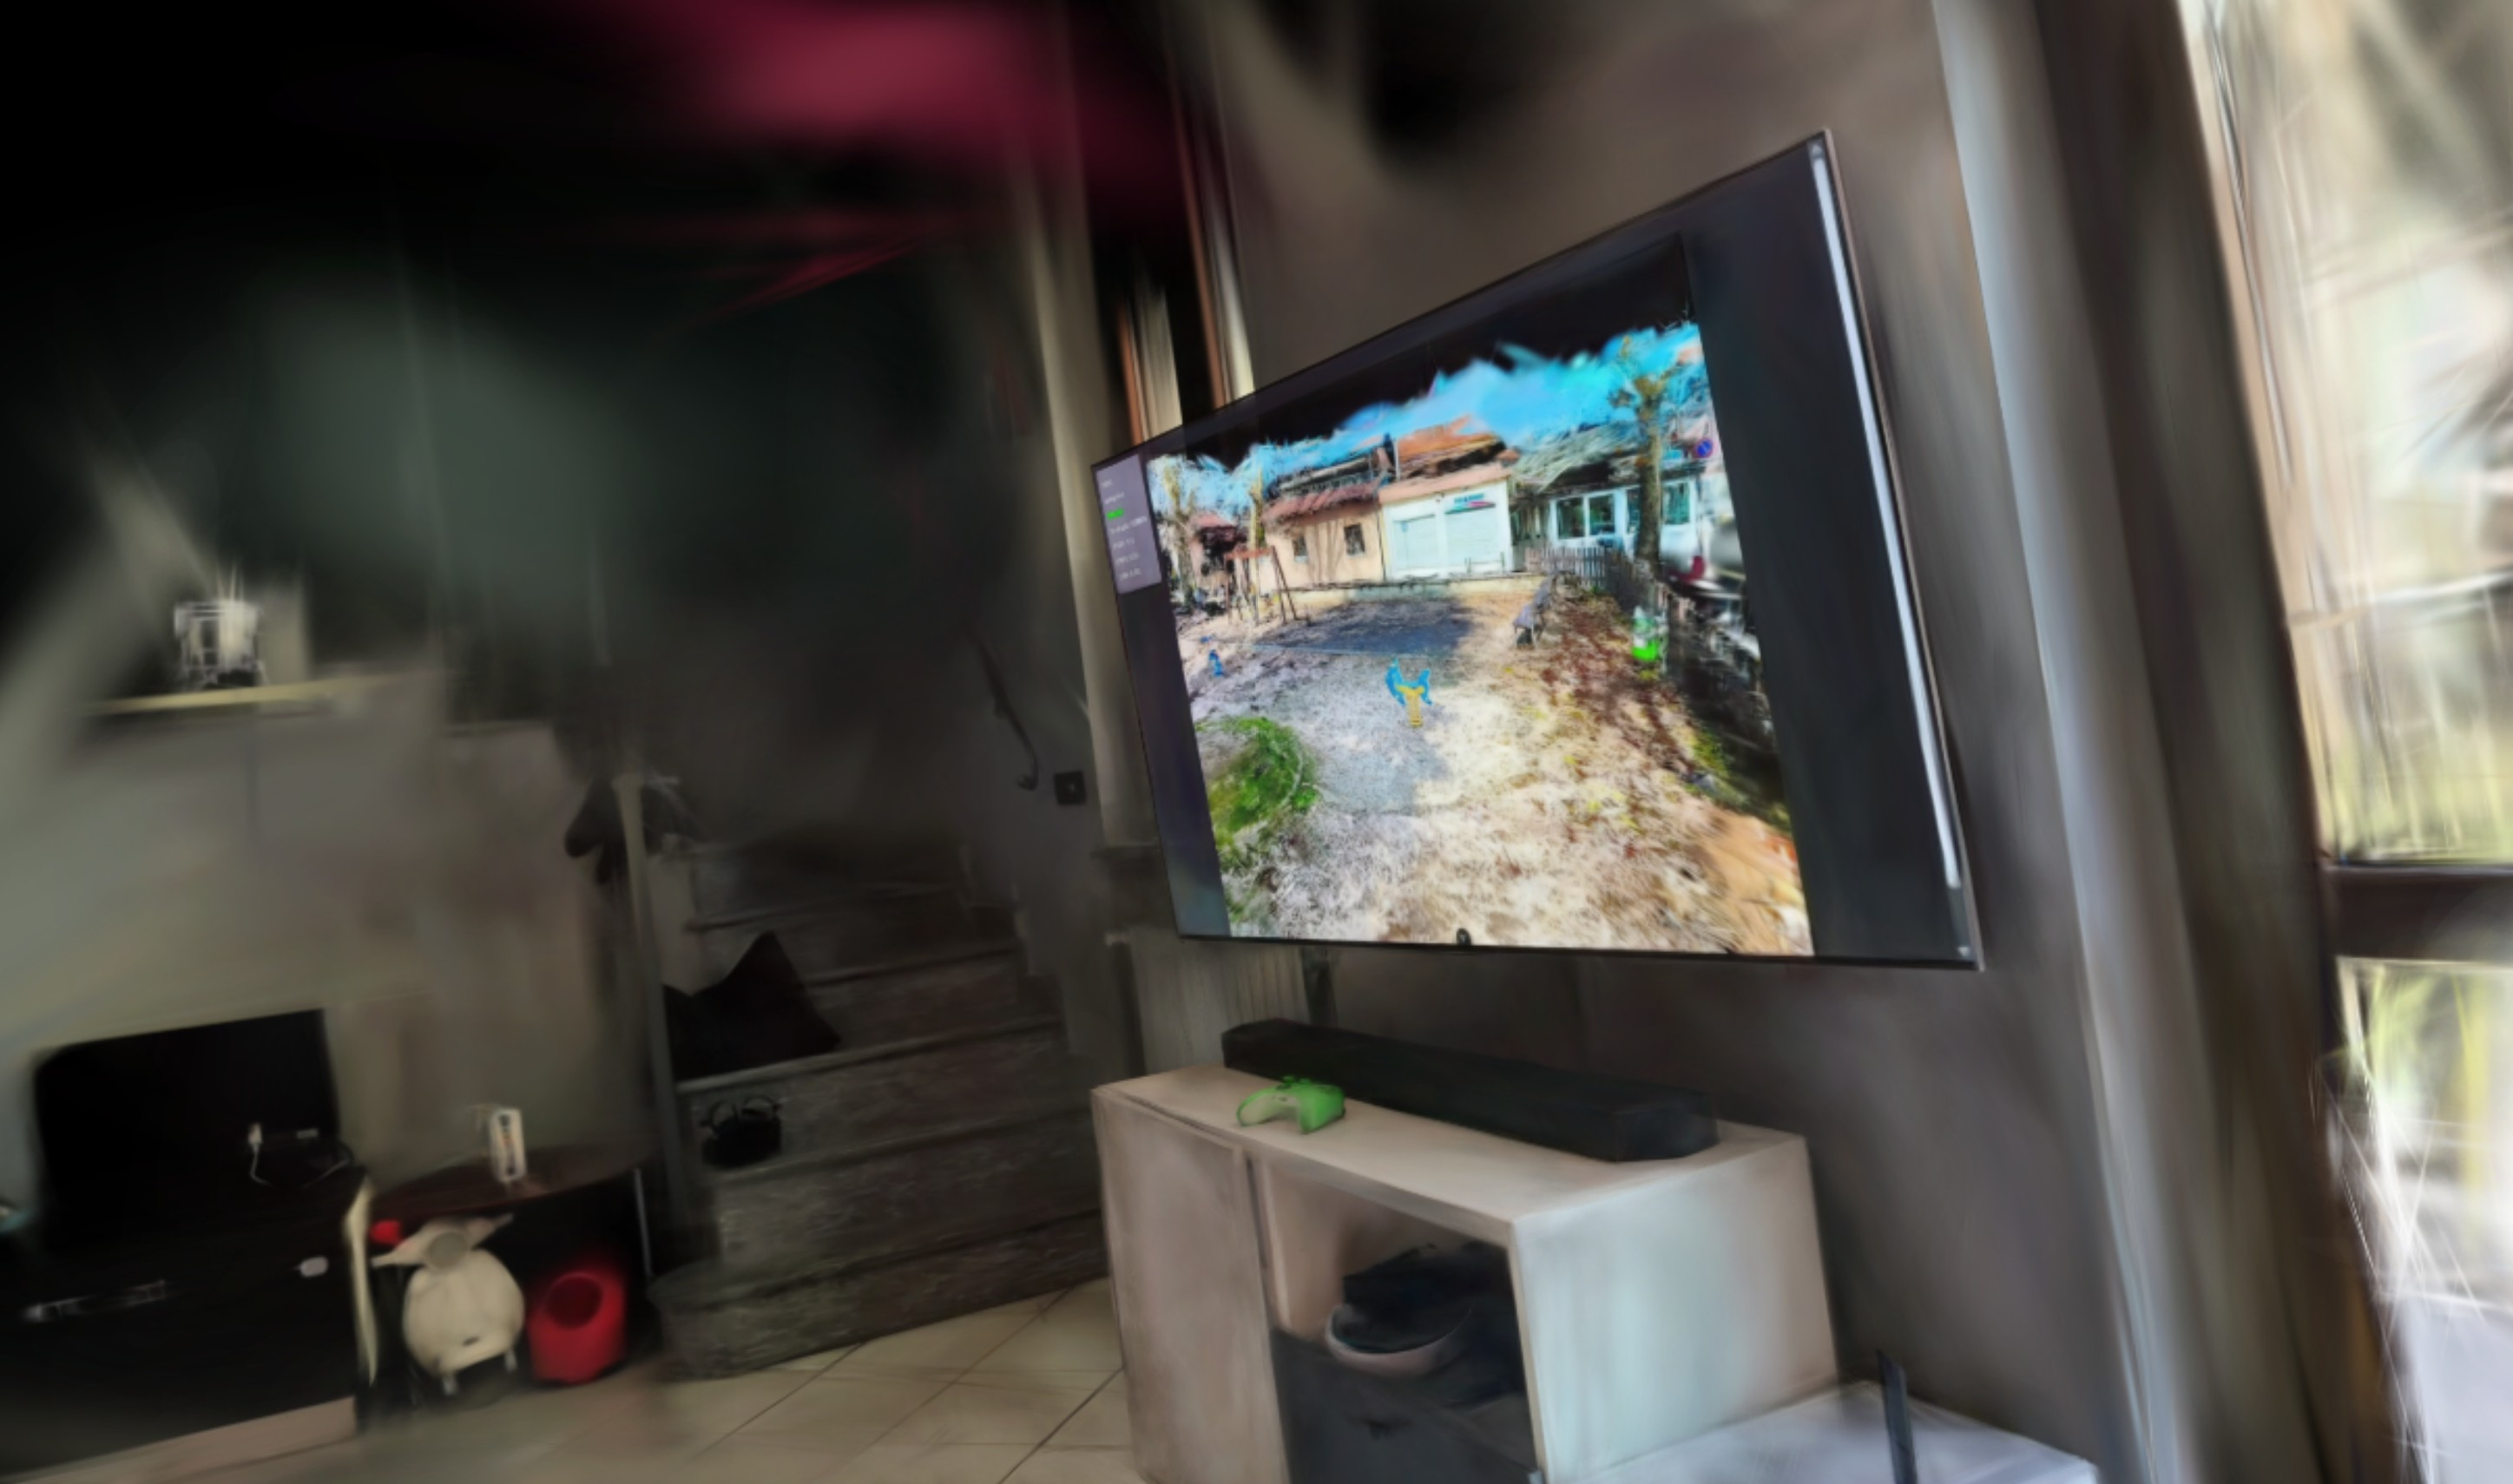
\includegraphics[width=0.32\textwidth,height=2.8cm,trim={80 40 80 40},clip]{images/benchmarks/my_workstation_mcmc_balanced_2.jpg}
	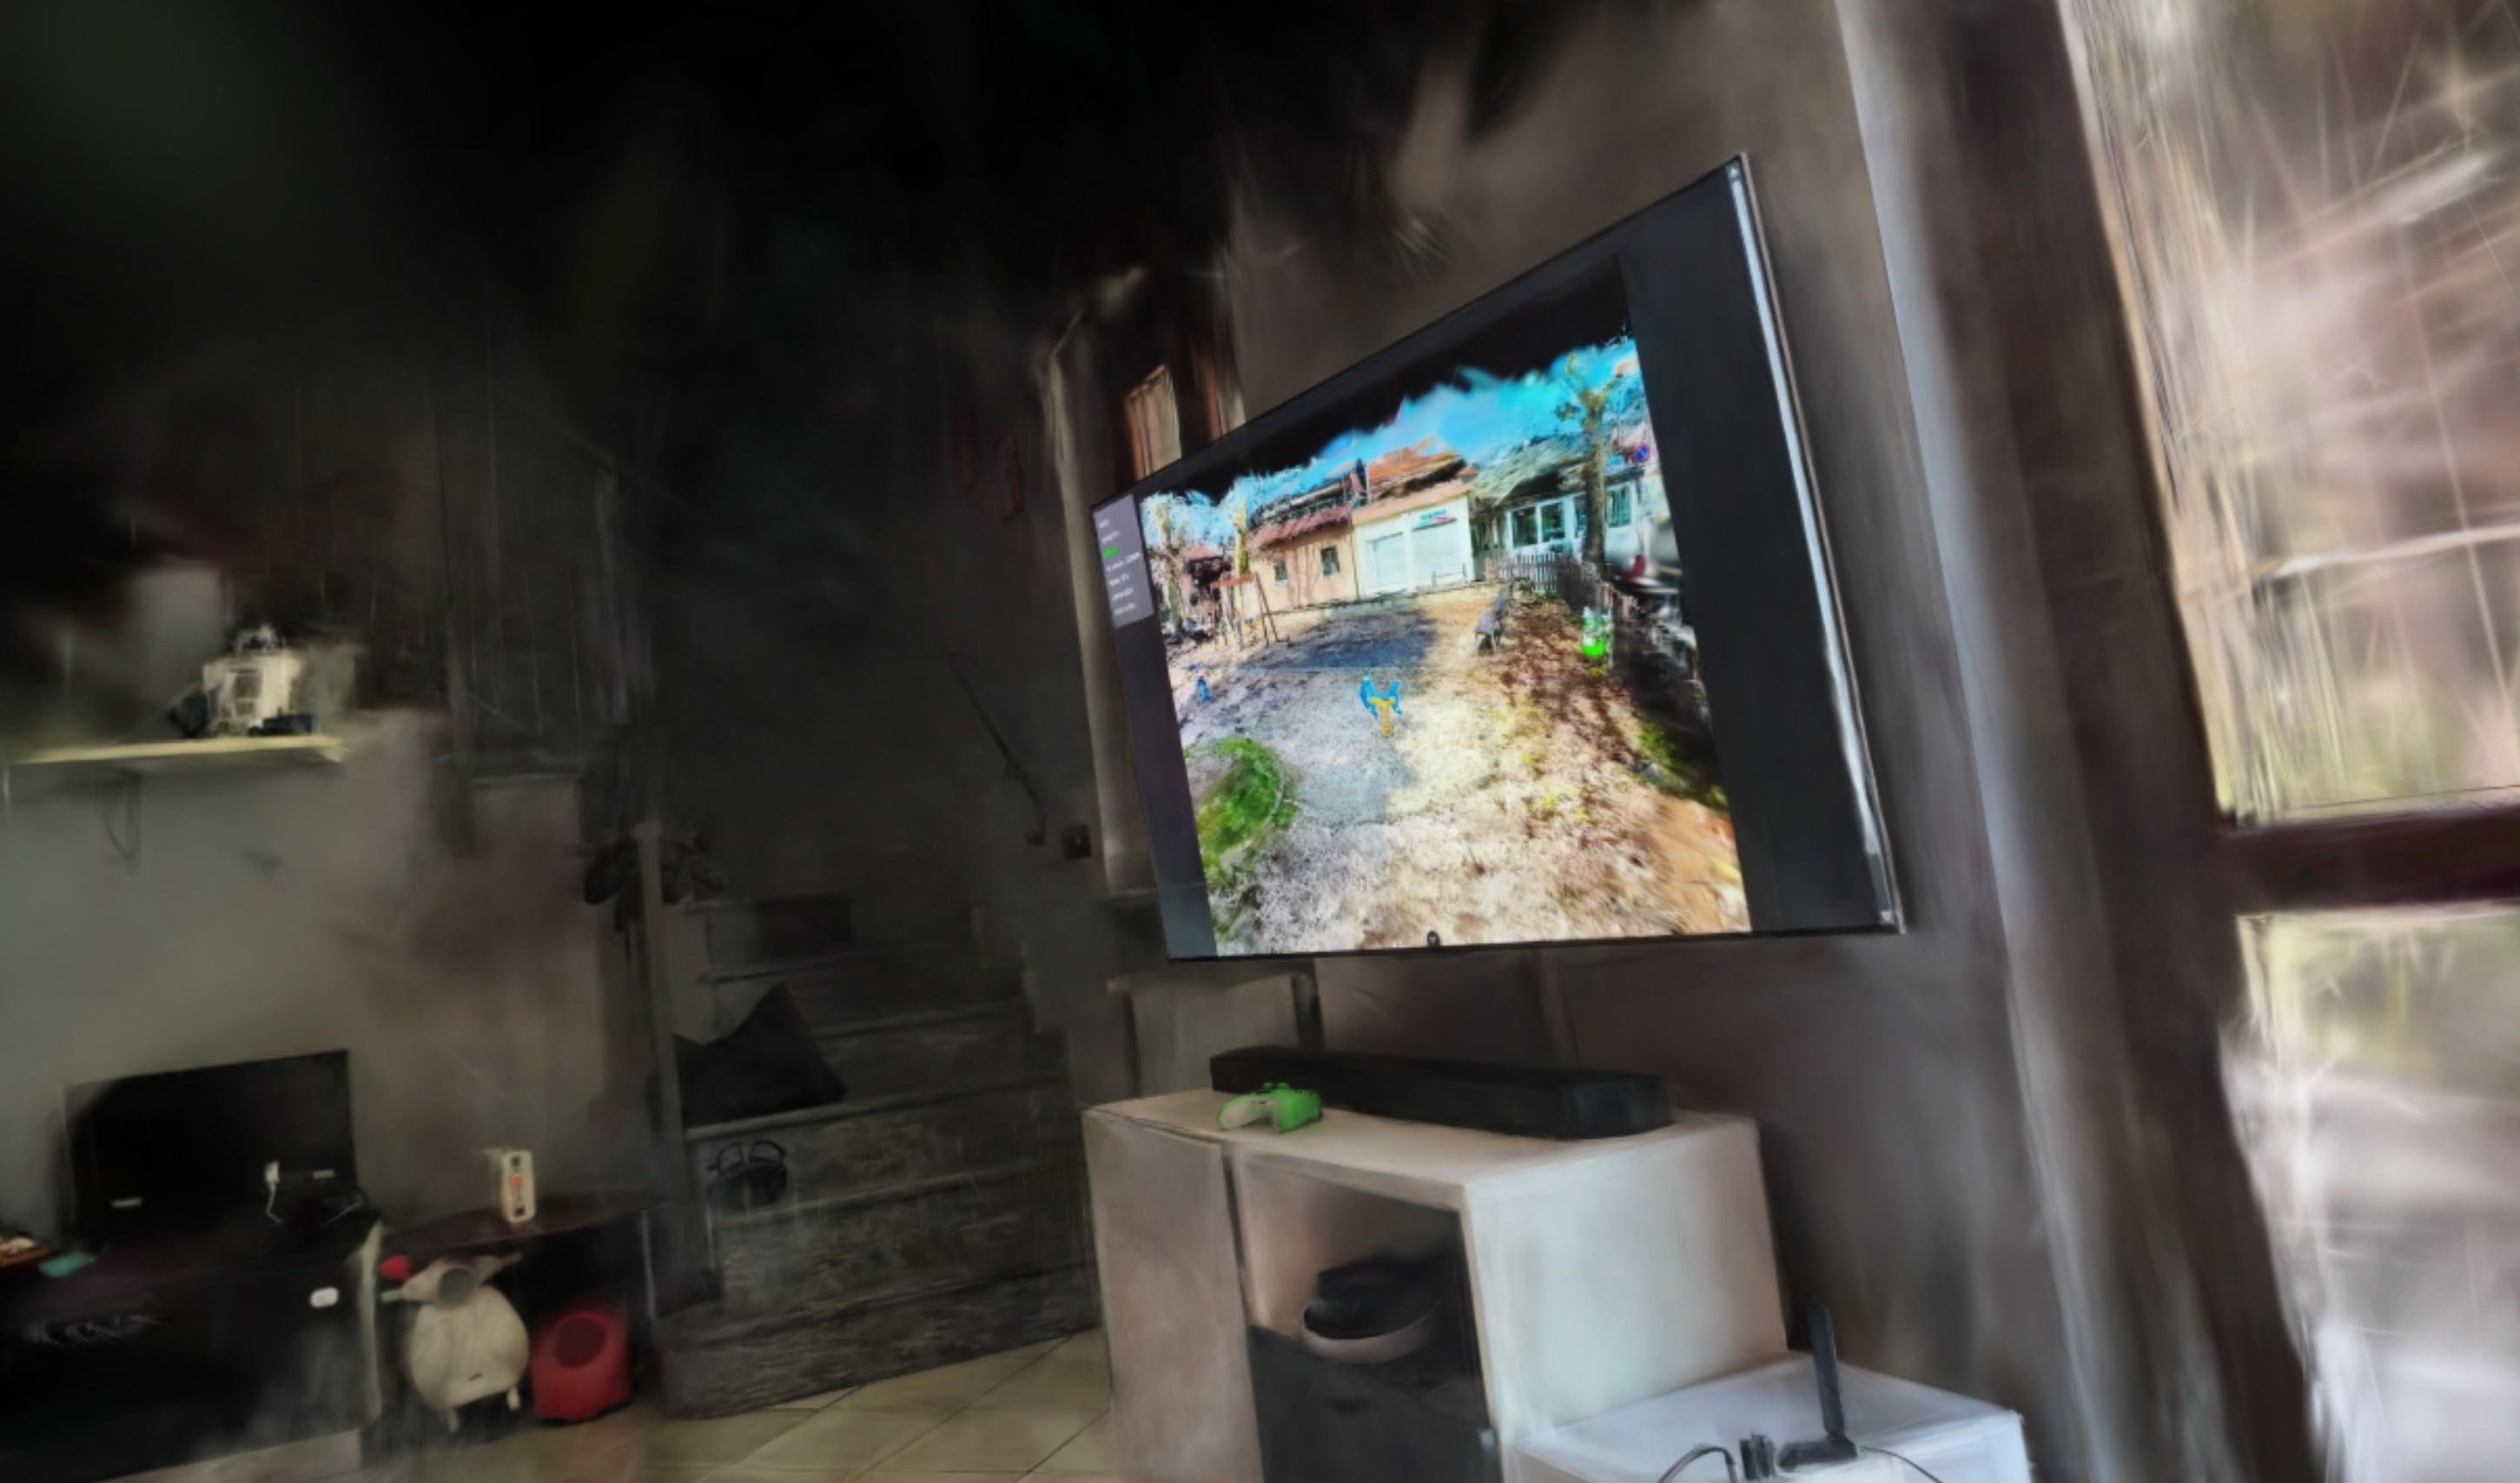
\includegraphics[width=0.32\textwidth,height=2.8cm,trim={80 40 80 40},clip]{images/benchmarks/my_workstation_taming_balanced_2.jpg}
	\caption{Confronto visivo My workstation (crop centrale) -- INRIA / MCMC / Taming}
	\label{fig:my_workstation_comparison}
\end{figure}



\paragraph{Tabella comparativa qualitativa}
\begin{table}[H]
	\centering
	\caption{Sintesi qualitativa visuale (S1 \textit{Spring Rider} e S3 \textit{My Workstation})}
	\label{tab:benchmark1_quality_visual}
	\begin{tabularx}{\linewidth}{l >{\centering\arraybackslash}X >{\centering\arraybackslash}X >{\centering\arraybackslash}X}
		\toprule
		\textbf{Criterio} & \textbf{INRIA} & \textbf{MCMC} & \textbf{Taming} \\
		\midrule
		Nitidezza soggetto / oggetti vicini & \warn & \cmark & \cmark \\
		Fedeltà cromatica                   & \warn & \warn  & \cmark \\
		Dettagli sfondo                      & \warn & \cmark & \cmark \\
		Texture suolo / superfici            & \xmark & \warn  & \cmark \\
		Gestione periferia / transizioni     & \xmark & \warn  & \cmark \\
		Artefatti visibili                   & \warn & \xmark & \cmark \\
		\bottomrule
	\end{tabularx}
	\vspace{0.4em}
	\footnotesize
	Legenda: \cmark = punto di forza,\; \warn = adeguato,\; \xmark = debolezza.
\end{table}



% ---------------------------------------------------
\subsubsection*{4. Conclusioni operative}
\begin{itemize}
	\item \textbf{Taming 3DGS} -- Miglior compromesso tra qualità, velocità e stabilità: indicato per deploy web e produzione.
	\item \textbf{MCMC 3DGS} -- Potenziale qualitativo elevato, ma meno prevedibile in risorse e più lento: indicato per ricerca e scenari controllati.
	\item \textbf{INRIA} -- Baseline veloce e leggera: utile per prototipazione rapida o scene semplici.
\end{itemize}

% ---------------------------------------------------
\subsubsection*{5. Appendice visiva}

\paragraph{Artefatti MCMC}
\begin{figure}[H]
	\centering
	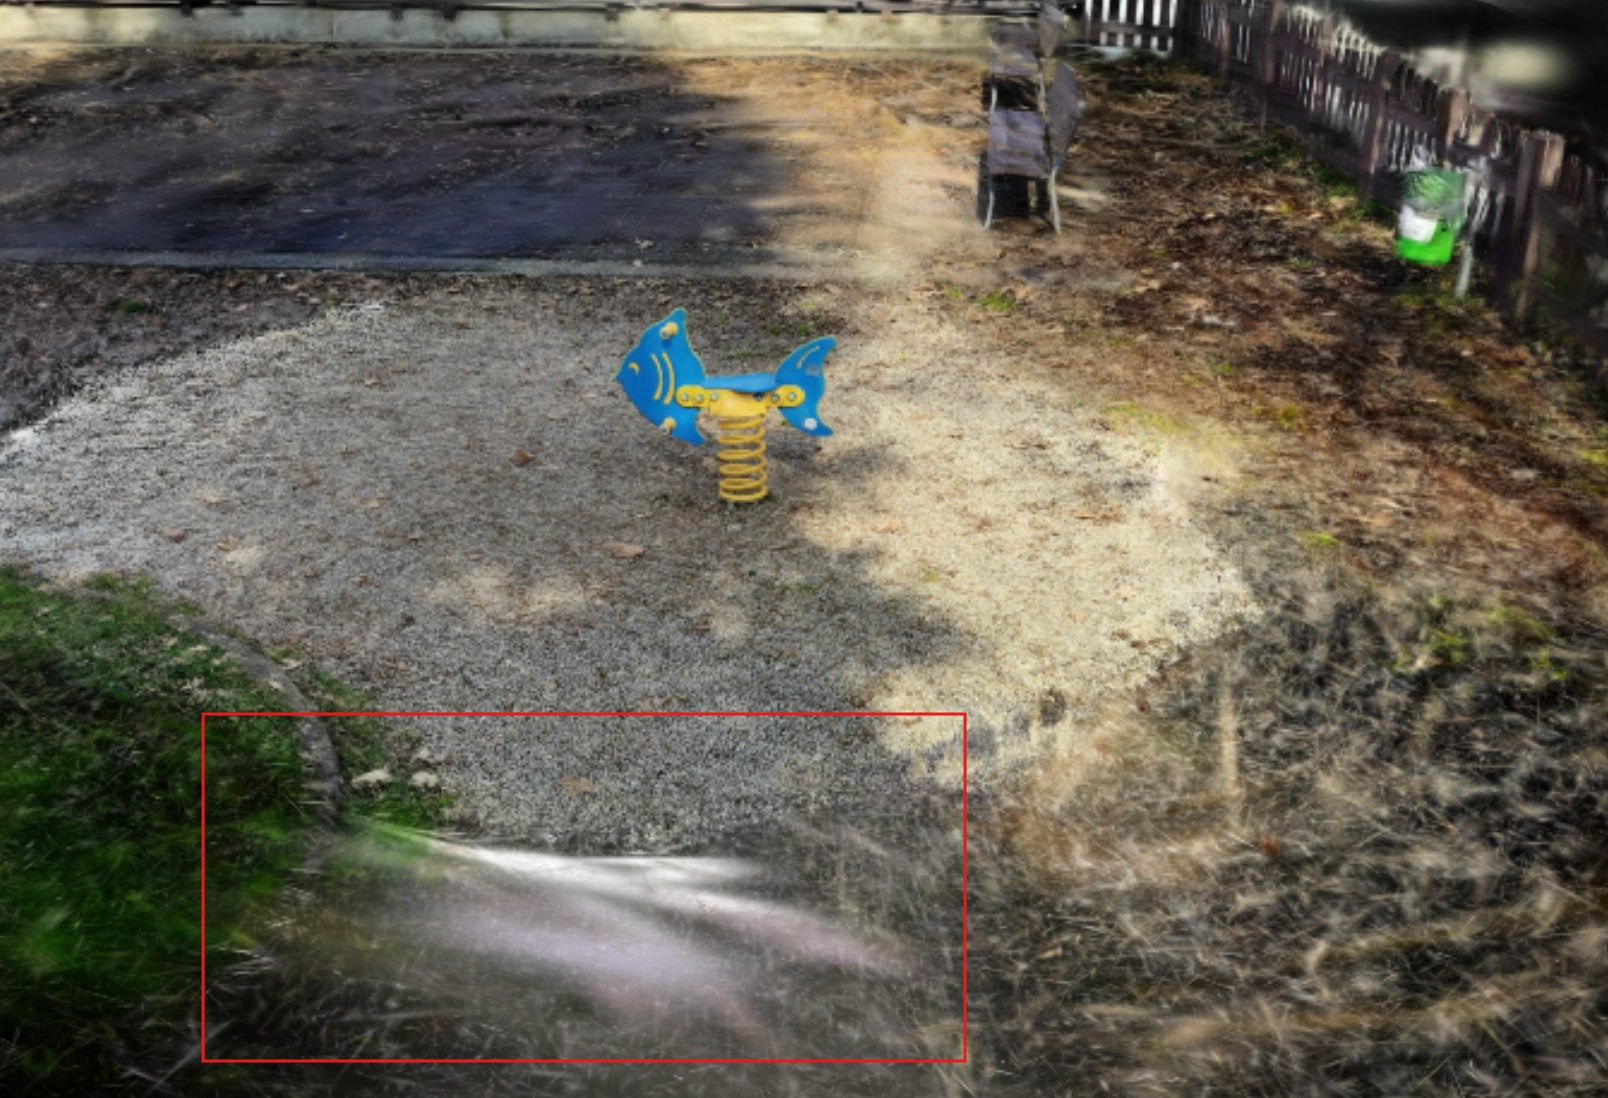
\includegraphics[width=0.49\textwidth,height=4cm,trim={80 40 80 40},clip]{images/benchmarks/spring_rider_mcmc_defect.jpg}
	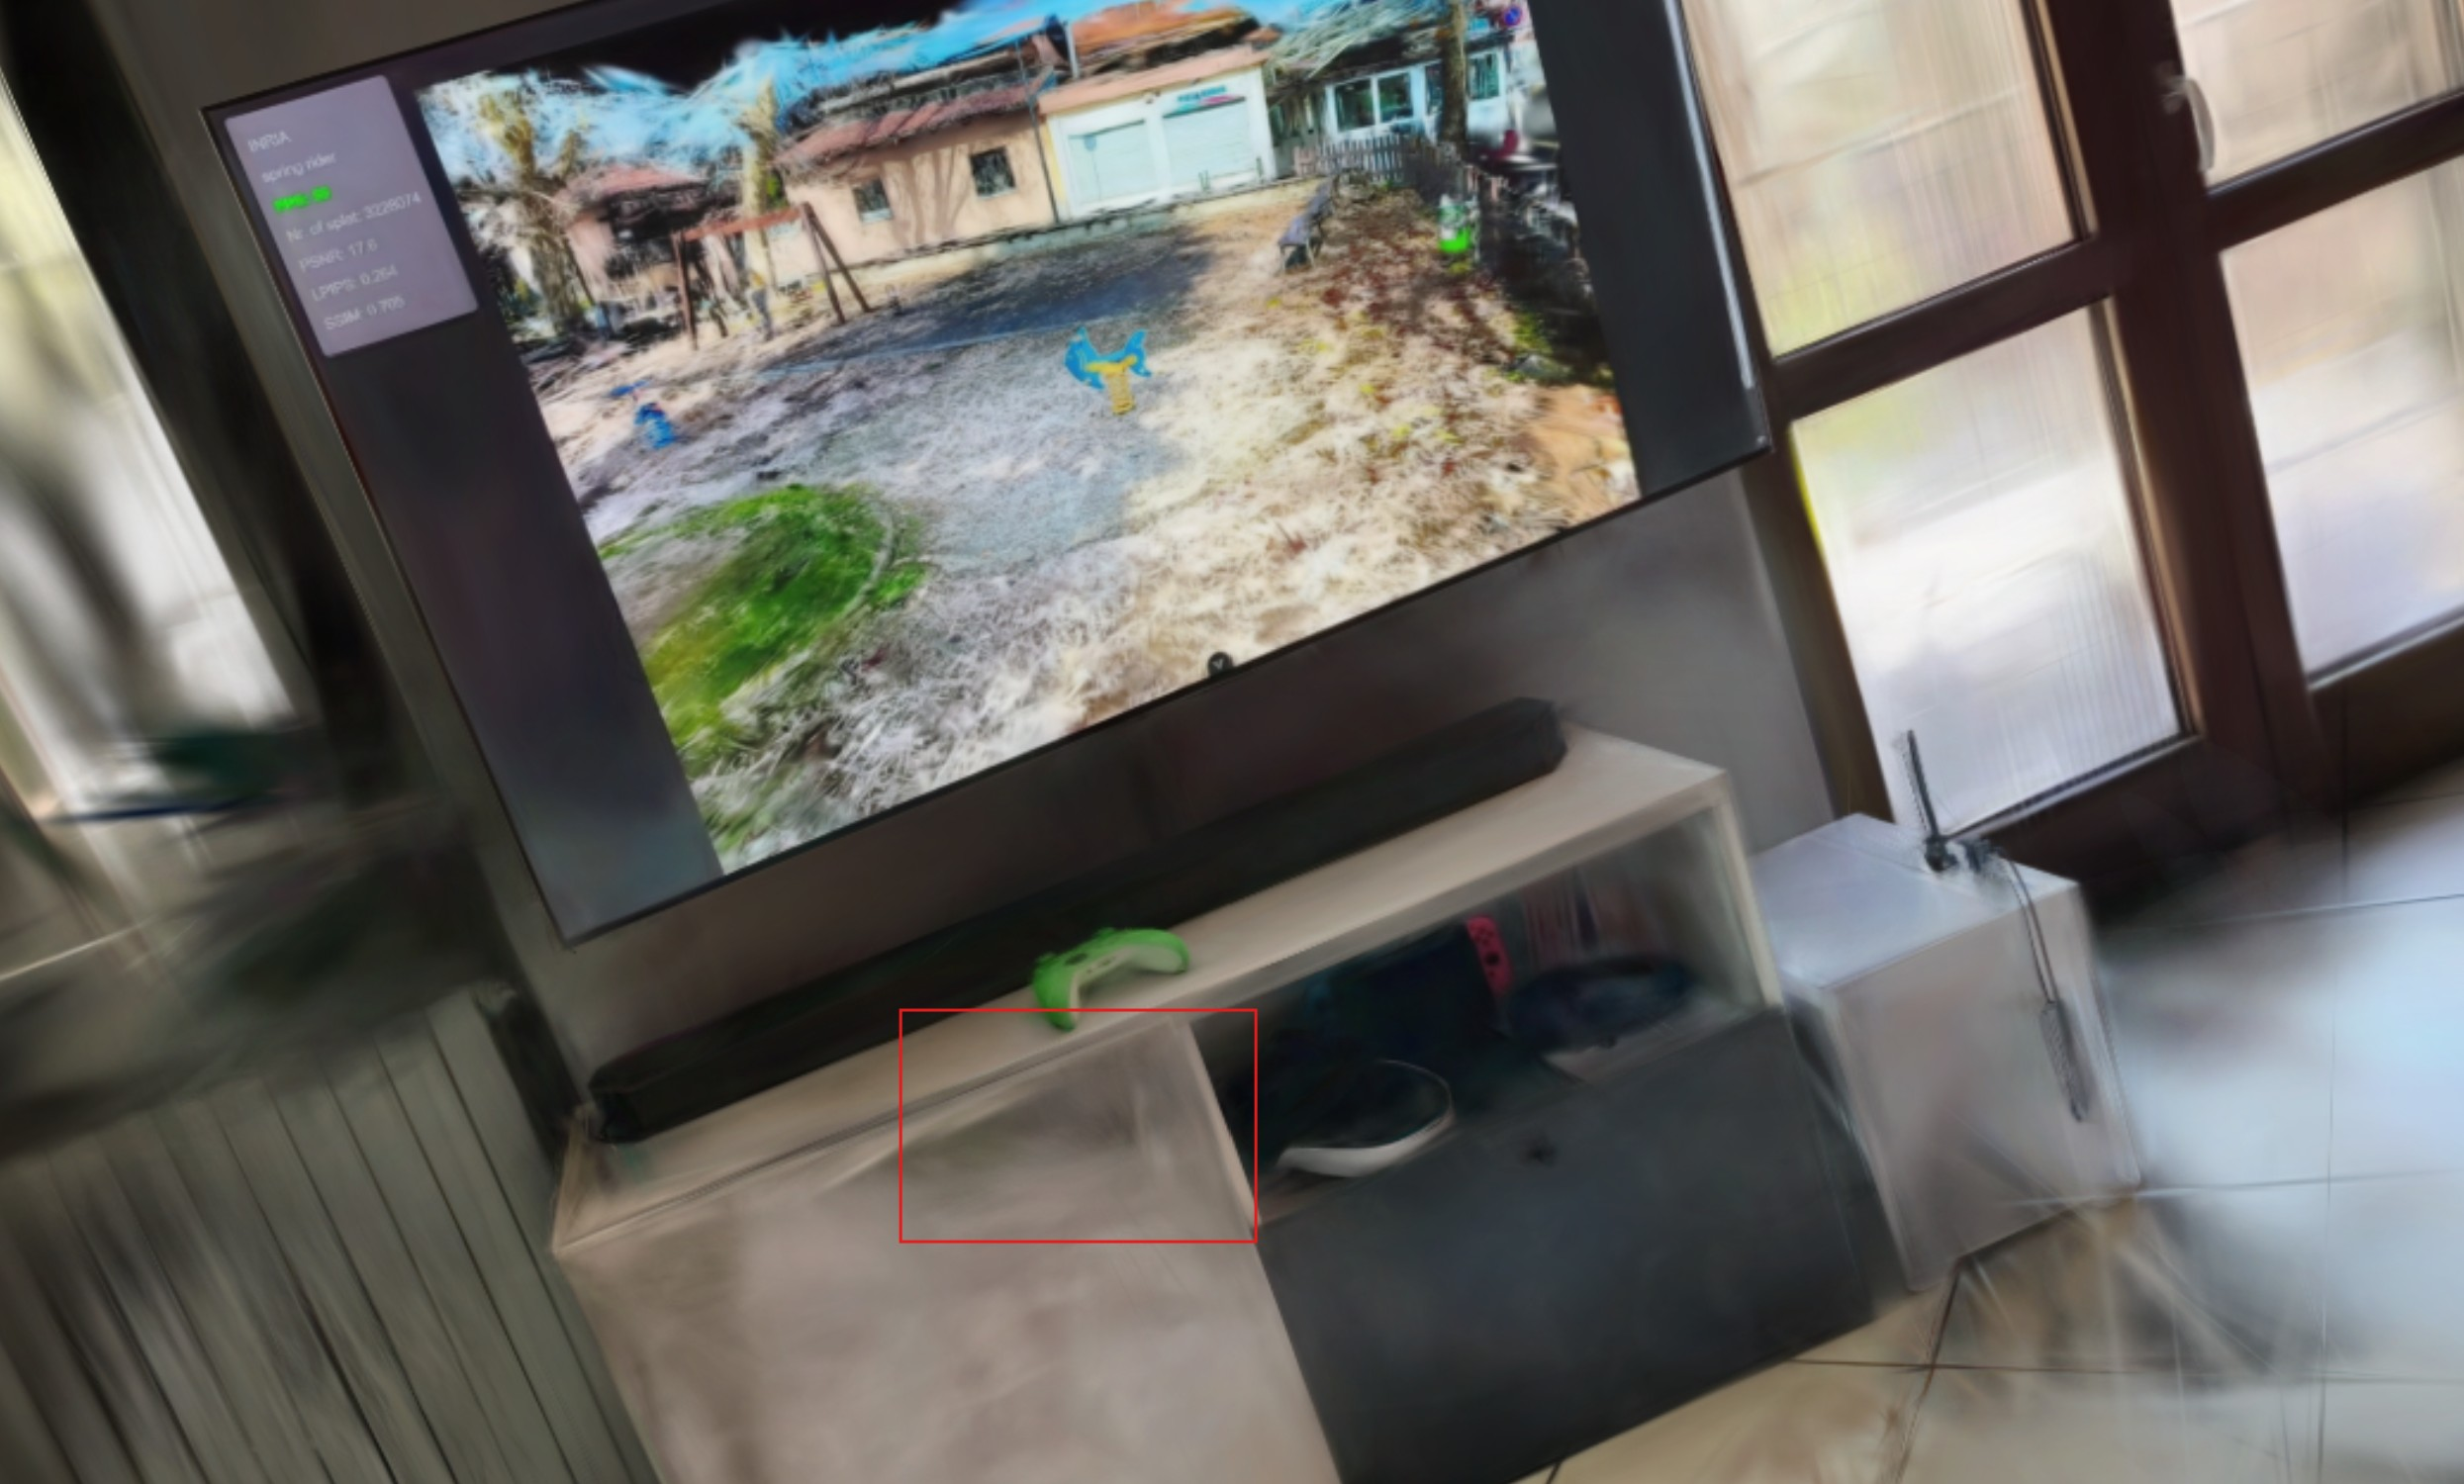
\includegraphics[width=0.49\textwidth,height=4cm,trim={80 40 80 40},clip]{images/benchmarks/my_workstation_mcmc_defect.jpg}
	\caption{Trasparenze anomale nei rendering MCMC}
	\label{fig:mcmc_transparency_defects}
\end{figure}

\paragraph{Esempio upscaling -- S2 Tomatoes}
\begin{figure}[H]
	\centering
	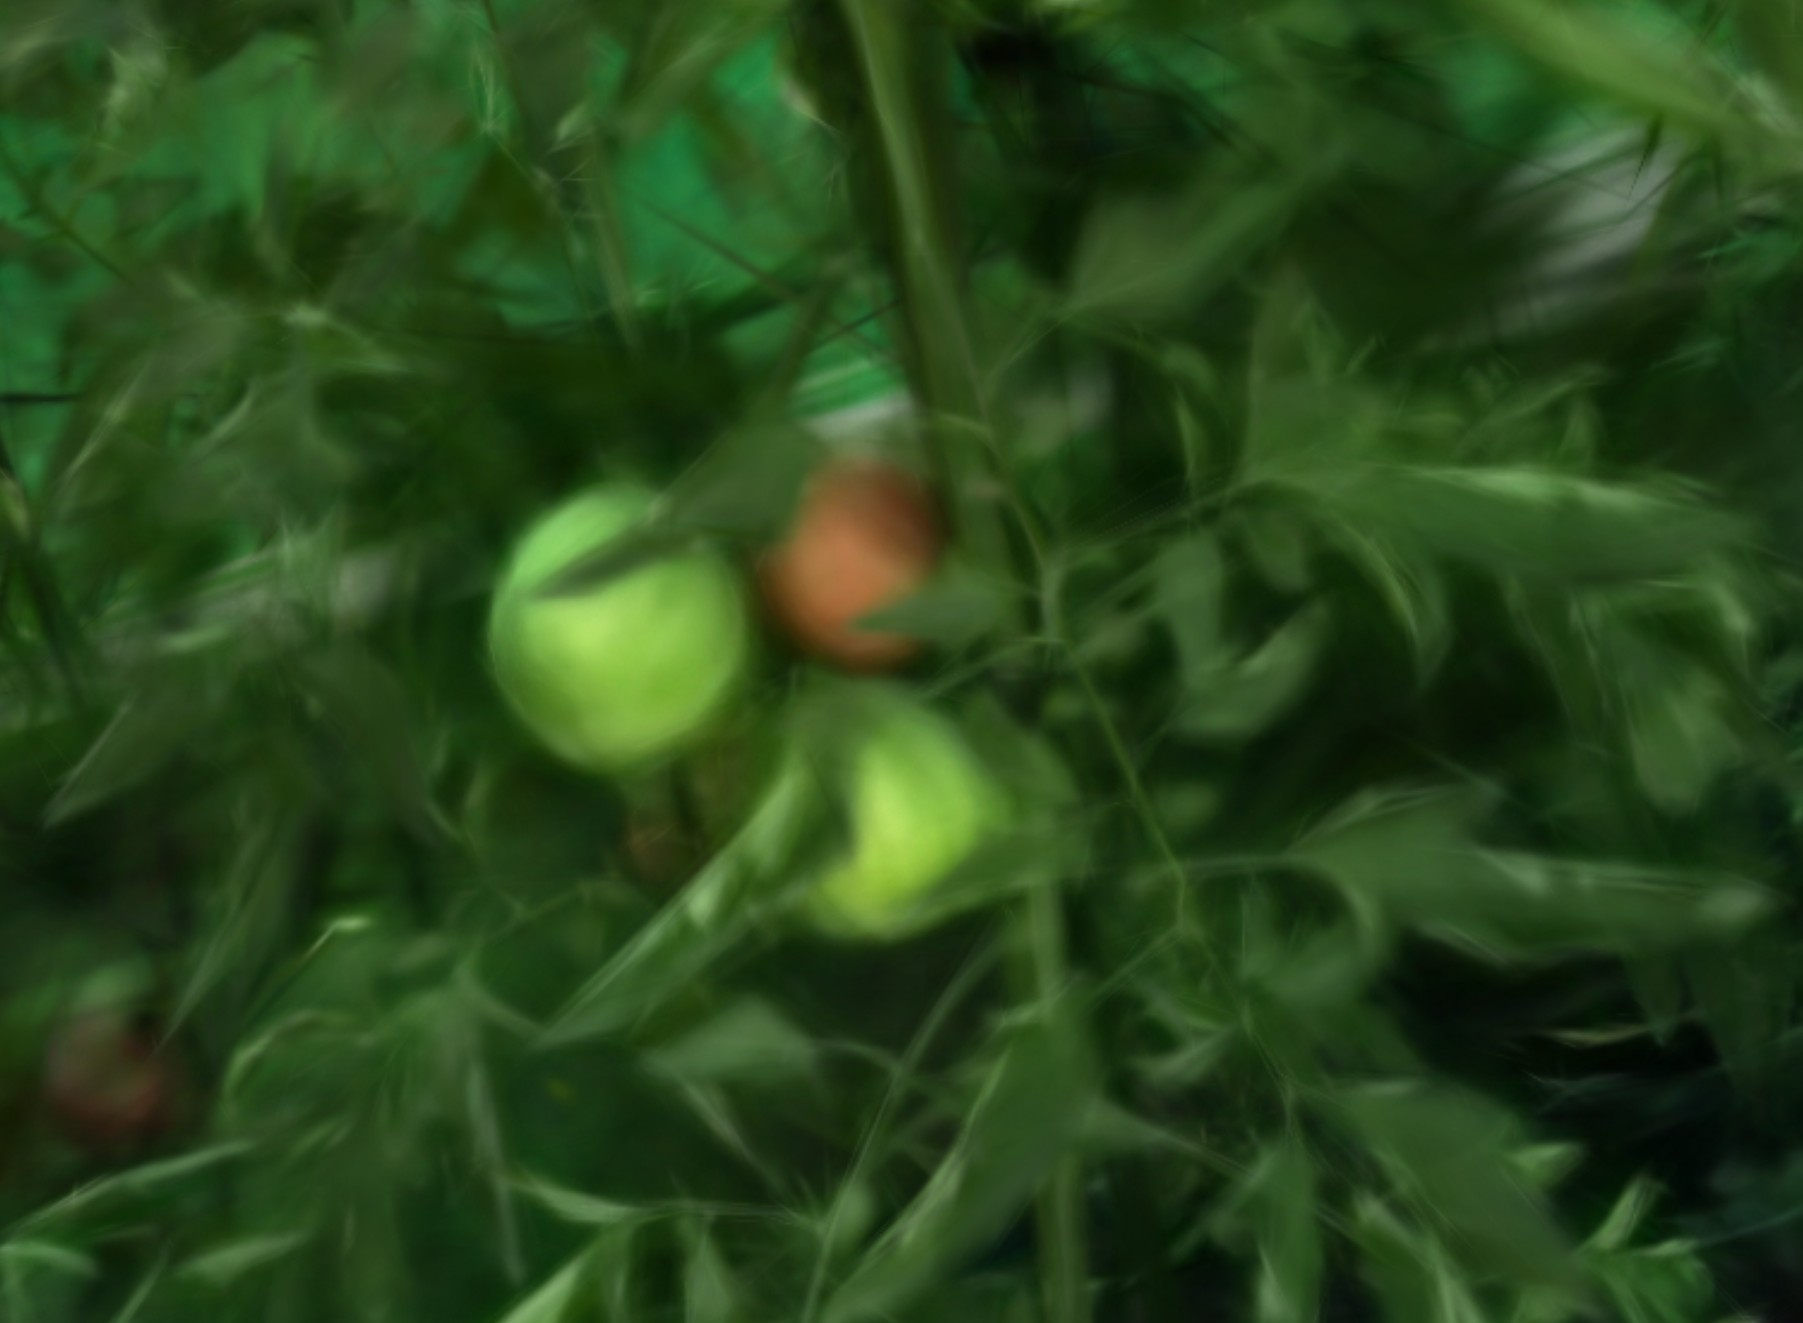
\includegraphics[width=0.32\textwidth,height=3.5cm,trim={80 40 80 40},clip]{images/benchmarks/tomatoes_480_mcmc.jpg}
	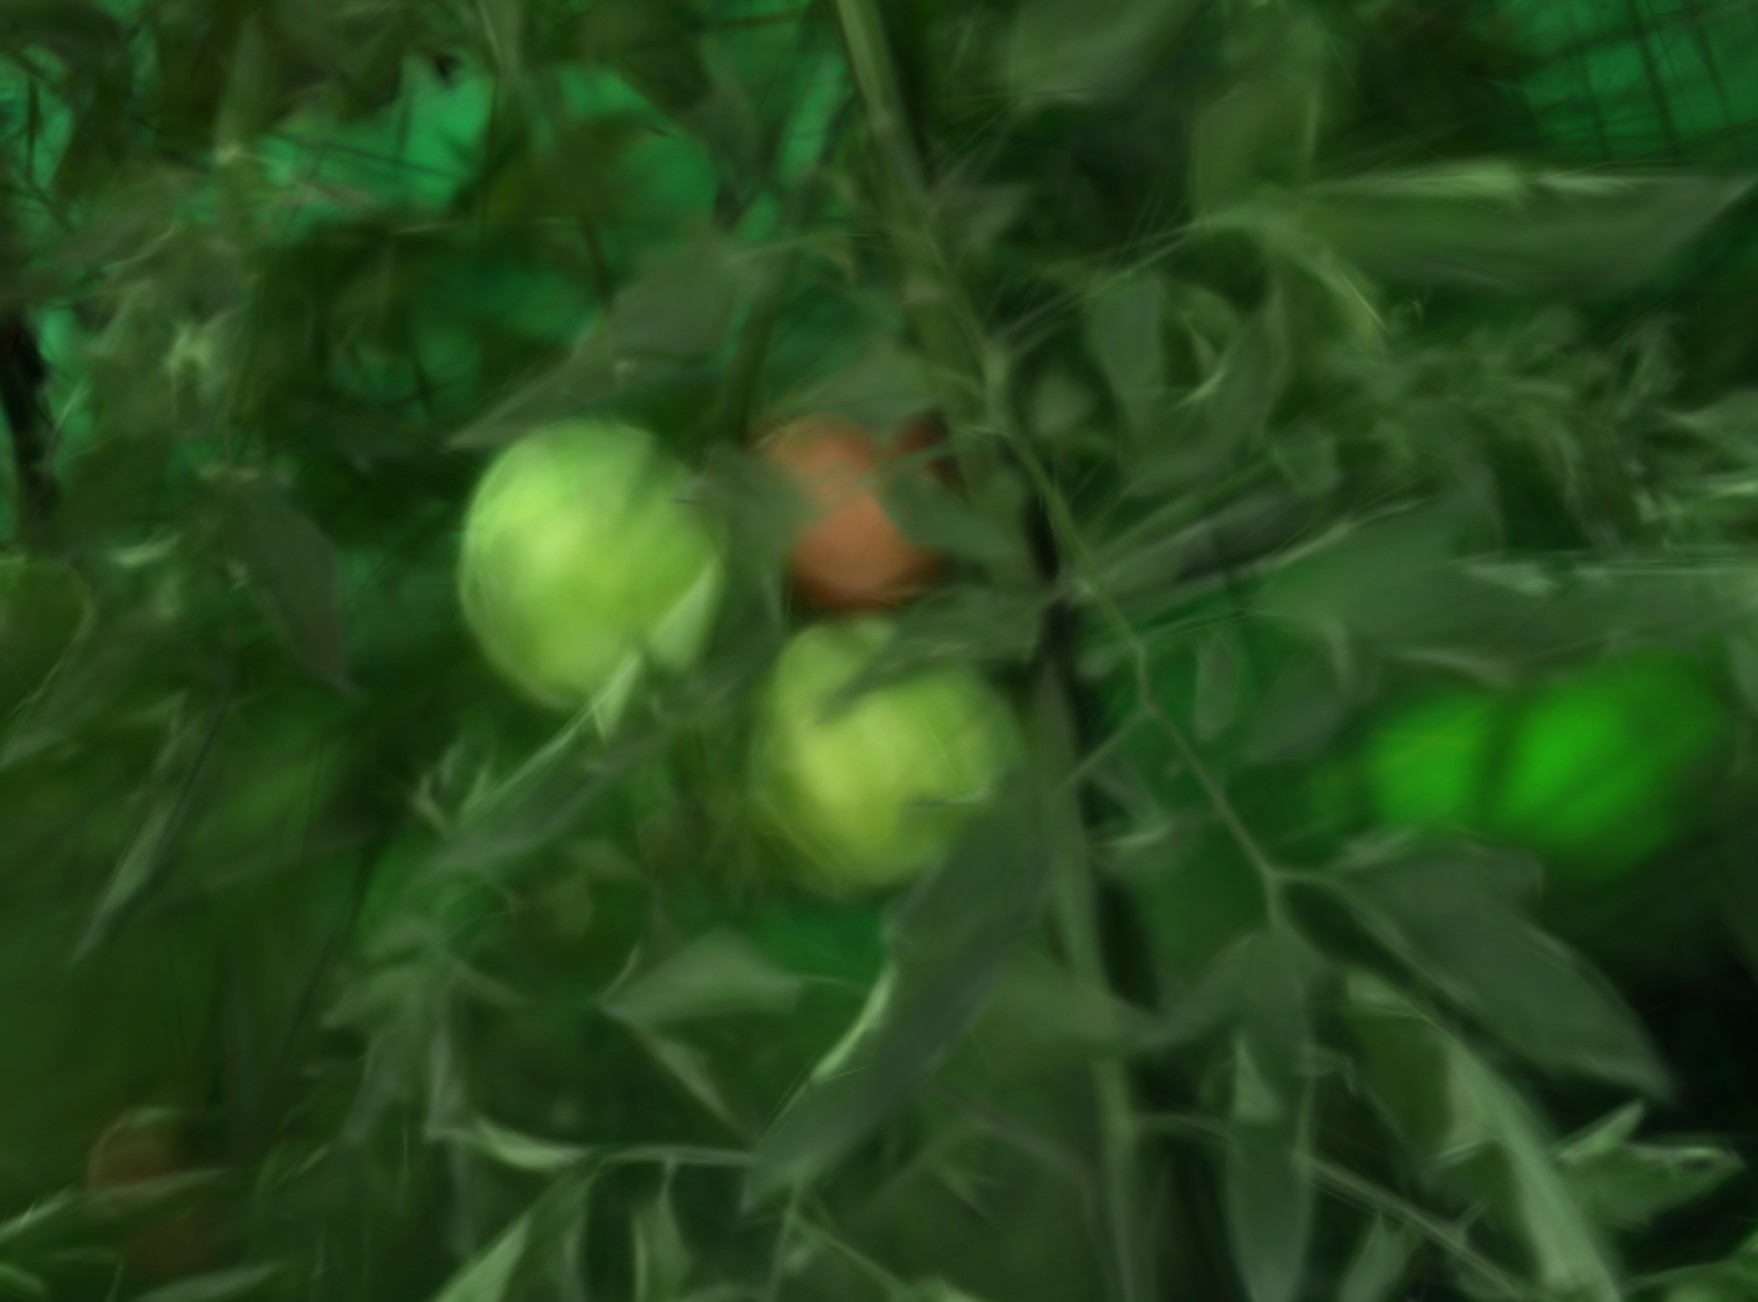
\includegraphics[width=0.32\textwidth,height=3.5cm,trim={80 40 80 40},clip]{images/benchmarks/tomatoes_720_mcmc.jpg}
	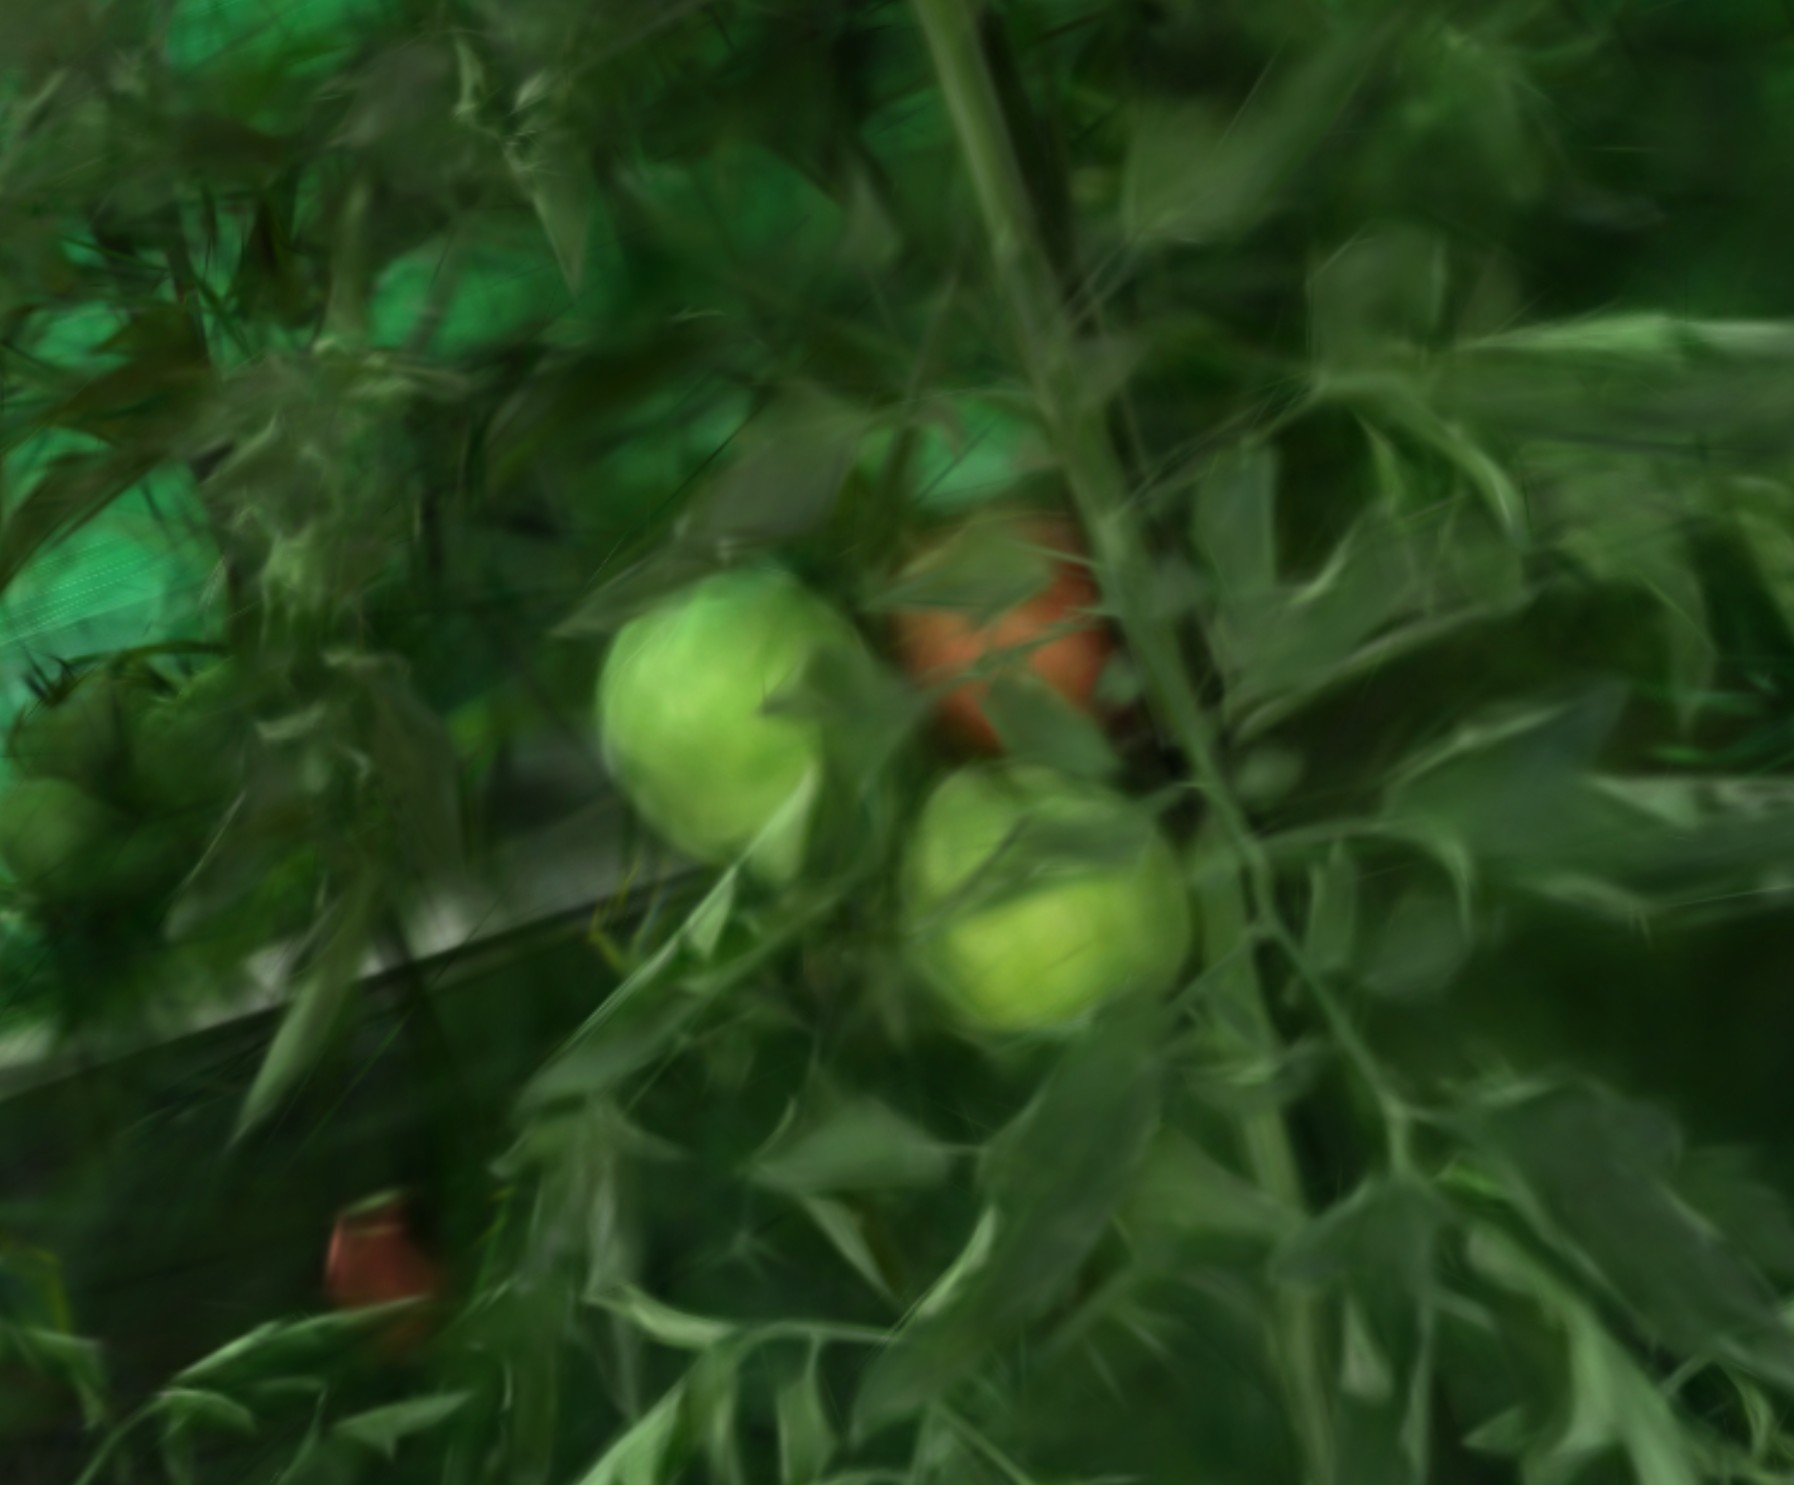
\includegraphics[width=0.32\textwidth,height=3.5cm,trim={80 40 80 40},clip]{images/benchmarks/tomatoes_1080_mcmc.jpg}
	\caption{Upscaling Tomatoes: 480p → 720p → 1080p (MCMC)}
	\label{fig:tomatoes_resolution_comparison}
\end{figure}



\subsection{Benchmark 2: Confronto tra livelli di qualit\`a (Taming 3DGS)}
\label{subsec:benchmark2_quality_levels}

\paragraph{Obiettivo}
Valutare il trade-off tra qualit\`a visiva, tempi di elaborazione e utilizzo delle risorse
per i tre profili \textbf{Fast}, \textbf{Balanced} e \textbf{Quality} dell'algoritmo \textbf{Taming 3DGS}.

\paragraph{Metodologia}
I test sono stati condotti esclusivamente a \textbf{720p} a causa dei vincoli di VRAM, 
variando soltanto due parametri:
\begin{itemize}
	\item \textbf{Iterations}: 20\,100 (Fast) $\rightarrow$ 25\,500 (Balanced) $\rightarrow$ 30\,000 (Quality)
	\item \textbf{Cams}: 10 $\rightarrow$ 20 $\rightarrow$ 30
\end{itemize}
Tutti i parametri di densificazione (\texttt{densify\_grad\_threshold}, \texttt{densification\_interval}, 
\texttt{densify\_until\_iter}) sono rimasti invariati per garantire stabilità e riproducibilità.

\paragraph{Scene di test}
\begin{itemize}
	\item \textbf{Lego Japanese Garden} -- geometrie regolari e dettagli architetturali.
	\item \textbf{Yellow Plant} -- scena naturale con texture organiche complesse.
\end{itemize}

\paragraph{Nota metodologica}
La scelta di una strategia conservativa (variazione di soli due parametri) deriva 
dall’osservazione che i parametri di densificazione possono avere effetti non lineari, 
scena-dipendenti e talvolta degradanti, aumentando il rischio di instabilità numerica.

% ---------------------- RISULTATI LEGO ----------------------
\begin{table}[H]
	\centering
	\caption{Lego Japanese Garden @ 720p -- confronto livelli di qualit\`a (Taming)}
	\label{tab:benchmark2_lego}
	\begin{tabularx}{0.92\linewidth}{l *{3}{>{\centering\arraybackslash}X}}
		\toprule
		\textbf{Metrica} & \textbf{Fast} & \textbf{Balanced} & \textbf{Quality} \\
		\midrule
		PSNR $\uparrow$         & 31.3 & 30.5 & 31.4 \\
		SSIM $\uparrow$         & 0.969 & 0.967 & 0.969 \\
		LPIPS $\downarrow$      & 0.102 & 0.103 & 0.103 \\
		Gaussiane               & 359K & 370K & 355K \\
		Tempo                   & 7m 19s & 8m 57s & 11m 22s \\
		Avg VRAM (GB)           & 7.61 & 9.16 & 8.26 \\
		Peak VRAM (GB)          & 9.47 & 12.20 & 11.74 \\
		Avg GPU (\%)            & 78.7 & 79.8 & 78.1 \\
		Max Temp (\,${}^\circ$C) & 72 & 73 & 73 \\
		\bottomrule
	\end{tabularx}
\end{table}

% ---------------------- RISULTATI YELLOW PLANT ----------------------
\begin{table}[H]
	\centering
	\caption{Yellow Plant @ 720p -- confronto livelli di qualit\`a (Taming)}
	\label{tab:benchmark2_yellow}
	\begin{tabularx}{0.92\linewidth}{l *{3}{>{\centering\arraybackslash}X}}
		\toprule
		\textbf{Metrica} & \textbf{Fast} & \textbf{Balanced} & \textbf{Quality} \\
		\midrule
		PSNR $\uparrow$         & 24.1 & 24.0 & 24.1 \\
		SSIM $\uparrow$         & 0.831 & 0.831 & 0.834 \\
		LPIPS $\downarrow$      & 0.146 & 0.143 & 0.142 \\
		Gaussiane               & 1.94M & 1.95M & 1.96M \\
		Tempo                   & 16m 48s & 20m 24s & 23m 50s \\
		Avg VRAM (GB)           & 9.70 & 11.50 & 11.43 \\
		Peak VRAM (GB)          & 11.84 & 13.67 & 9.92 \\
		Avg GPU (\%)            & 84.3 & 89.2 & 85.6 \\
		Max Temp (\,${}^\circ$C) & 69 & 69 & 70 \\
		\bottomrule
	\end{tabularx}
\end{table}

\paragraph{Lettura dei risultati}
Le differenze qualitative tra i tre livelli sono contenute: in \textit{Lego}, Fast e Quality
raggiungono entrambi un PSNR di circa 31.3--31.4, mentre Balanced risulta leggermente inferiore.
In \textit{Yellow Plant}, LPIPS migliora marginalmente in Quality ma l’incremento è modesto.
Il tempo di elaborazione cresce in modo significativo: \textbf{+55\%} per Quality rispetto a Fast
in \textit{Lego} e \textbf{+42\%} in \textit{Yellow Plant}.
La VRAM non mostra un andamento monotono e le temperature restano stabili (69--73\,${}^\circ$C).

\paragraph{Raccomandazione operativa}
\begin{itemize}
	\item \textbf{Fast} -- Profilo consigliato per deployment veloci: tempi ridotti del 35--50\% rispetto a Quality, con differenze metriche trascurabili.
	\item \textbf{Balanced} -- Poco utile con i settaggi attuali; può diventare rilevante solo se calibrato diversamente (es. densificazione intermedia).
	\item \textbf{Quality} -- Da usare solo quando il tempo non è un vincolo e si desidera massimizzare ogni punto percentuale di qualità.
\end{itemize}

% ---------------------- IMMAGINI LEGO ----------------------
\begin{figure}[H]
	\centering
	\begin{subfigure}{0.32\textwidth}
		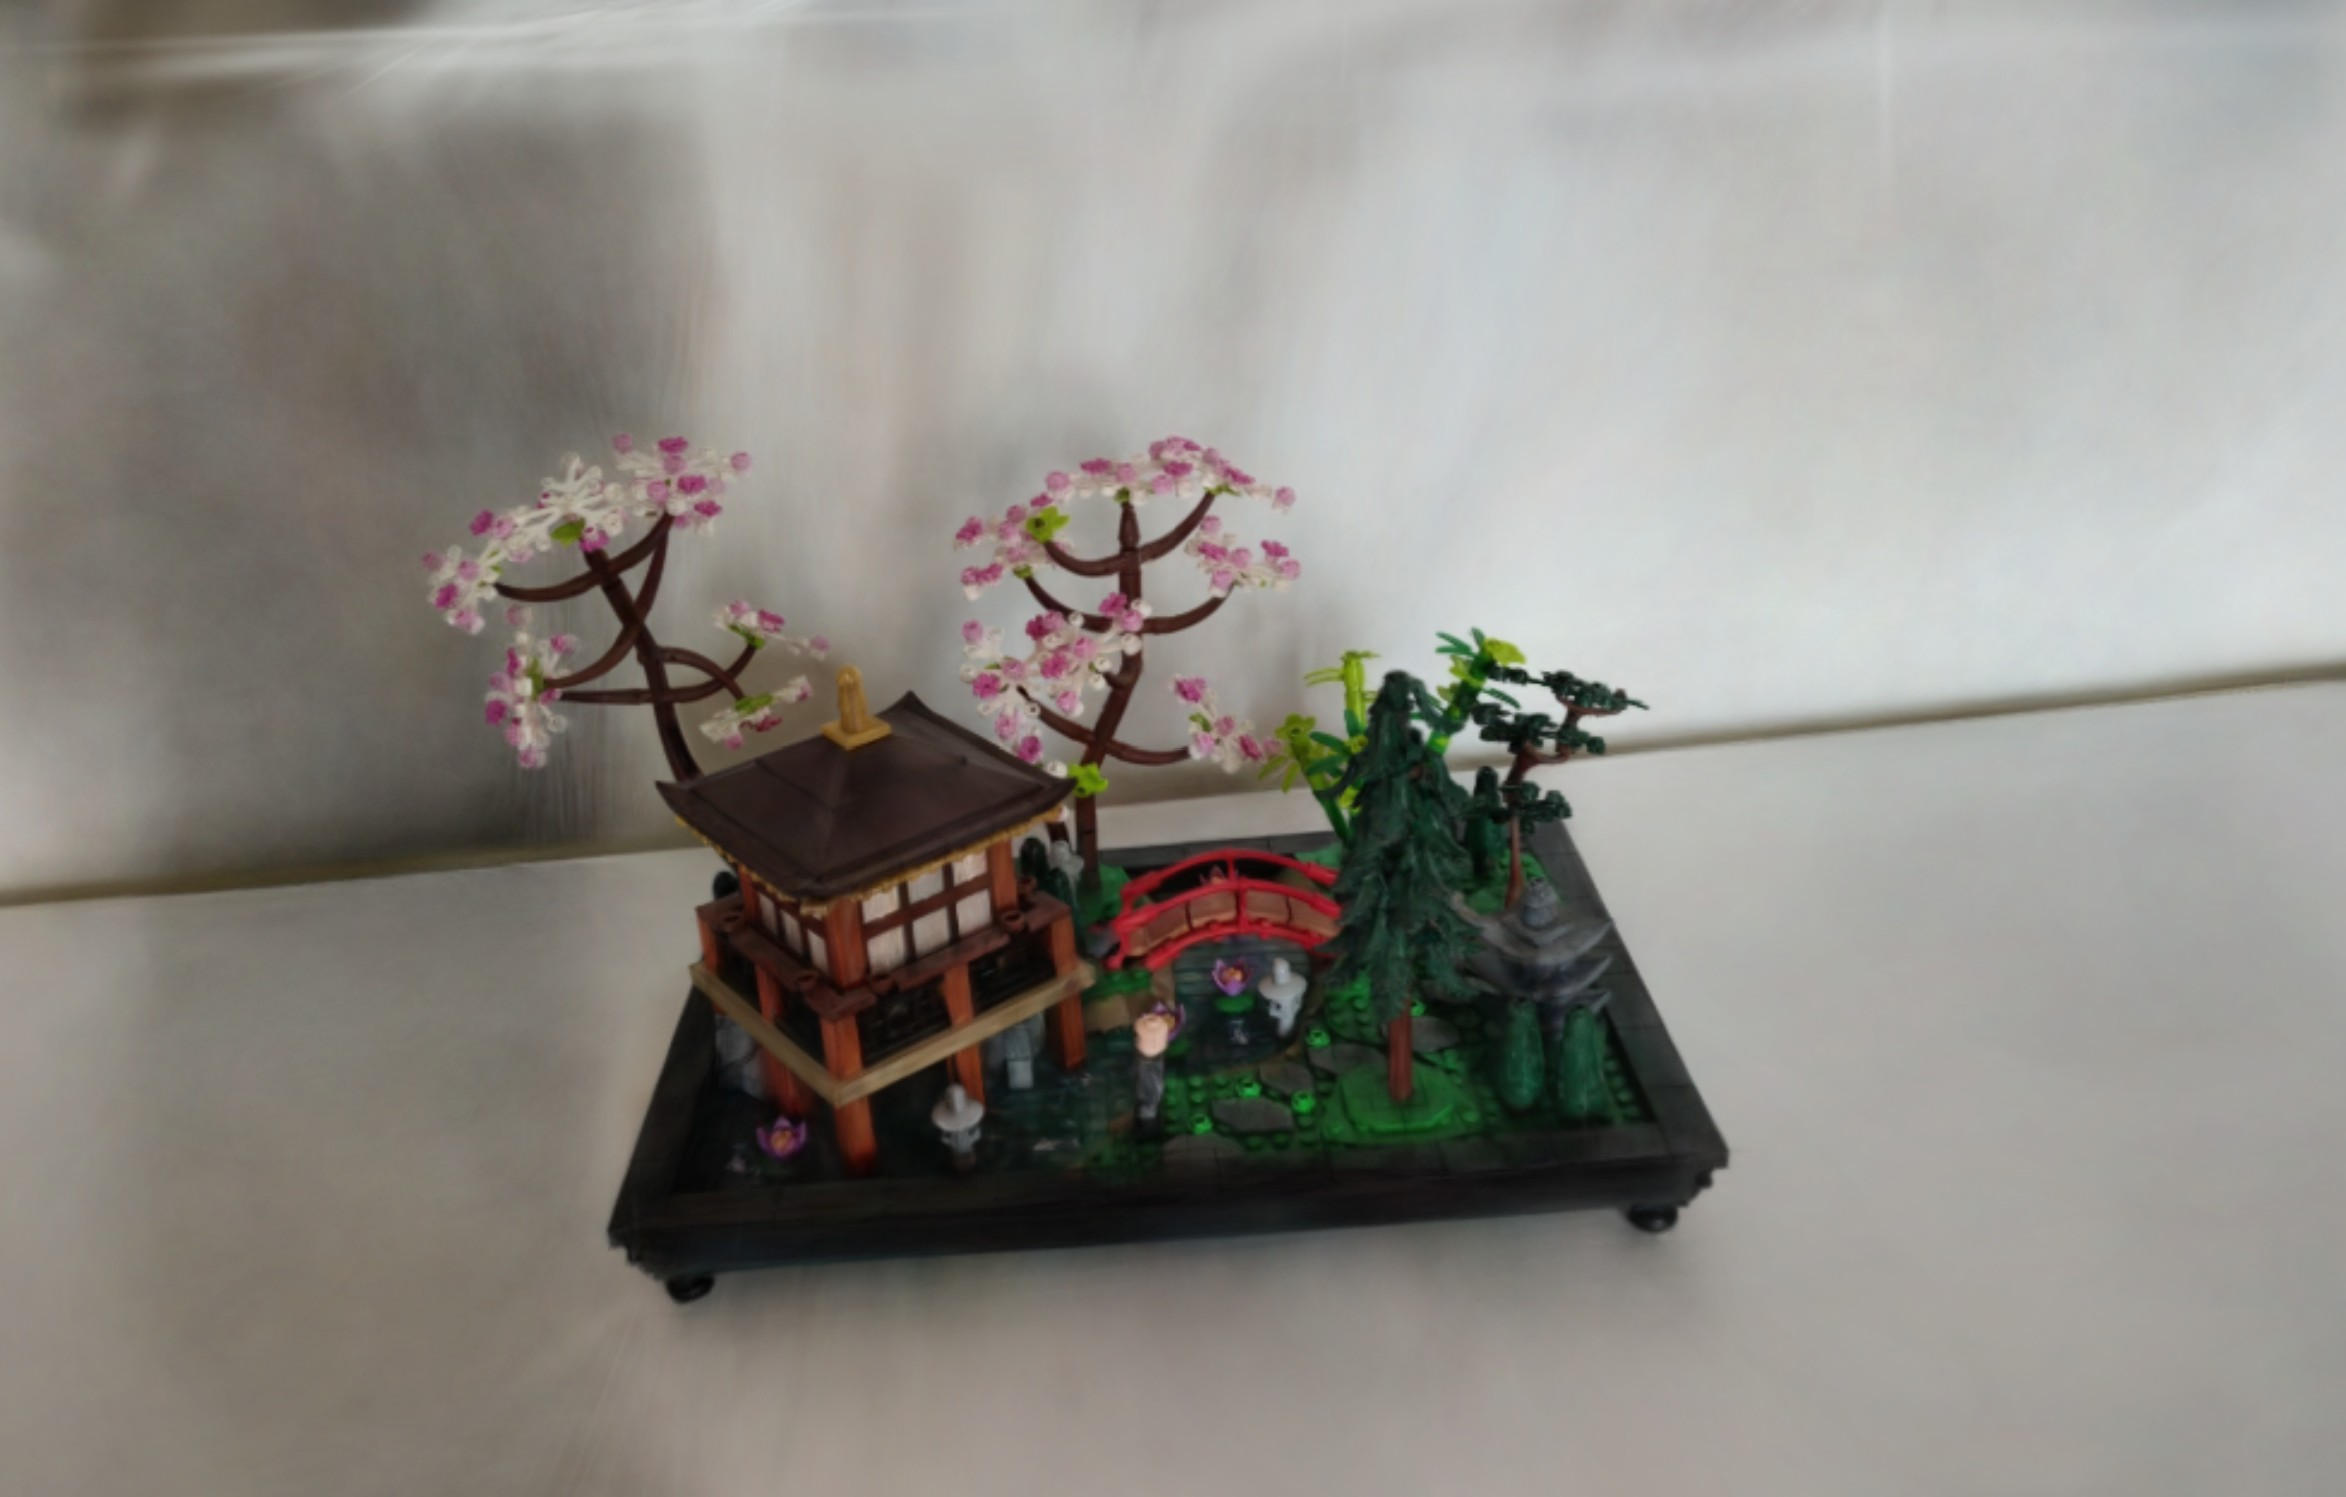
\includegraphics[width=\linewidth, height=2.3cm, trim={80 40 80 40}, clip]{images/benchmarks/lego_japanese_garden_taming_fast.jpg}
		\caption{Fast}
	\end{subfigure}
	\hfill
	\begin{subfigure}{0.32\textwidth}
		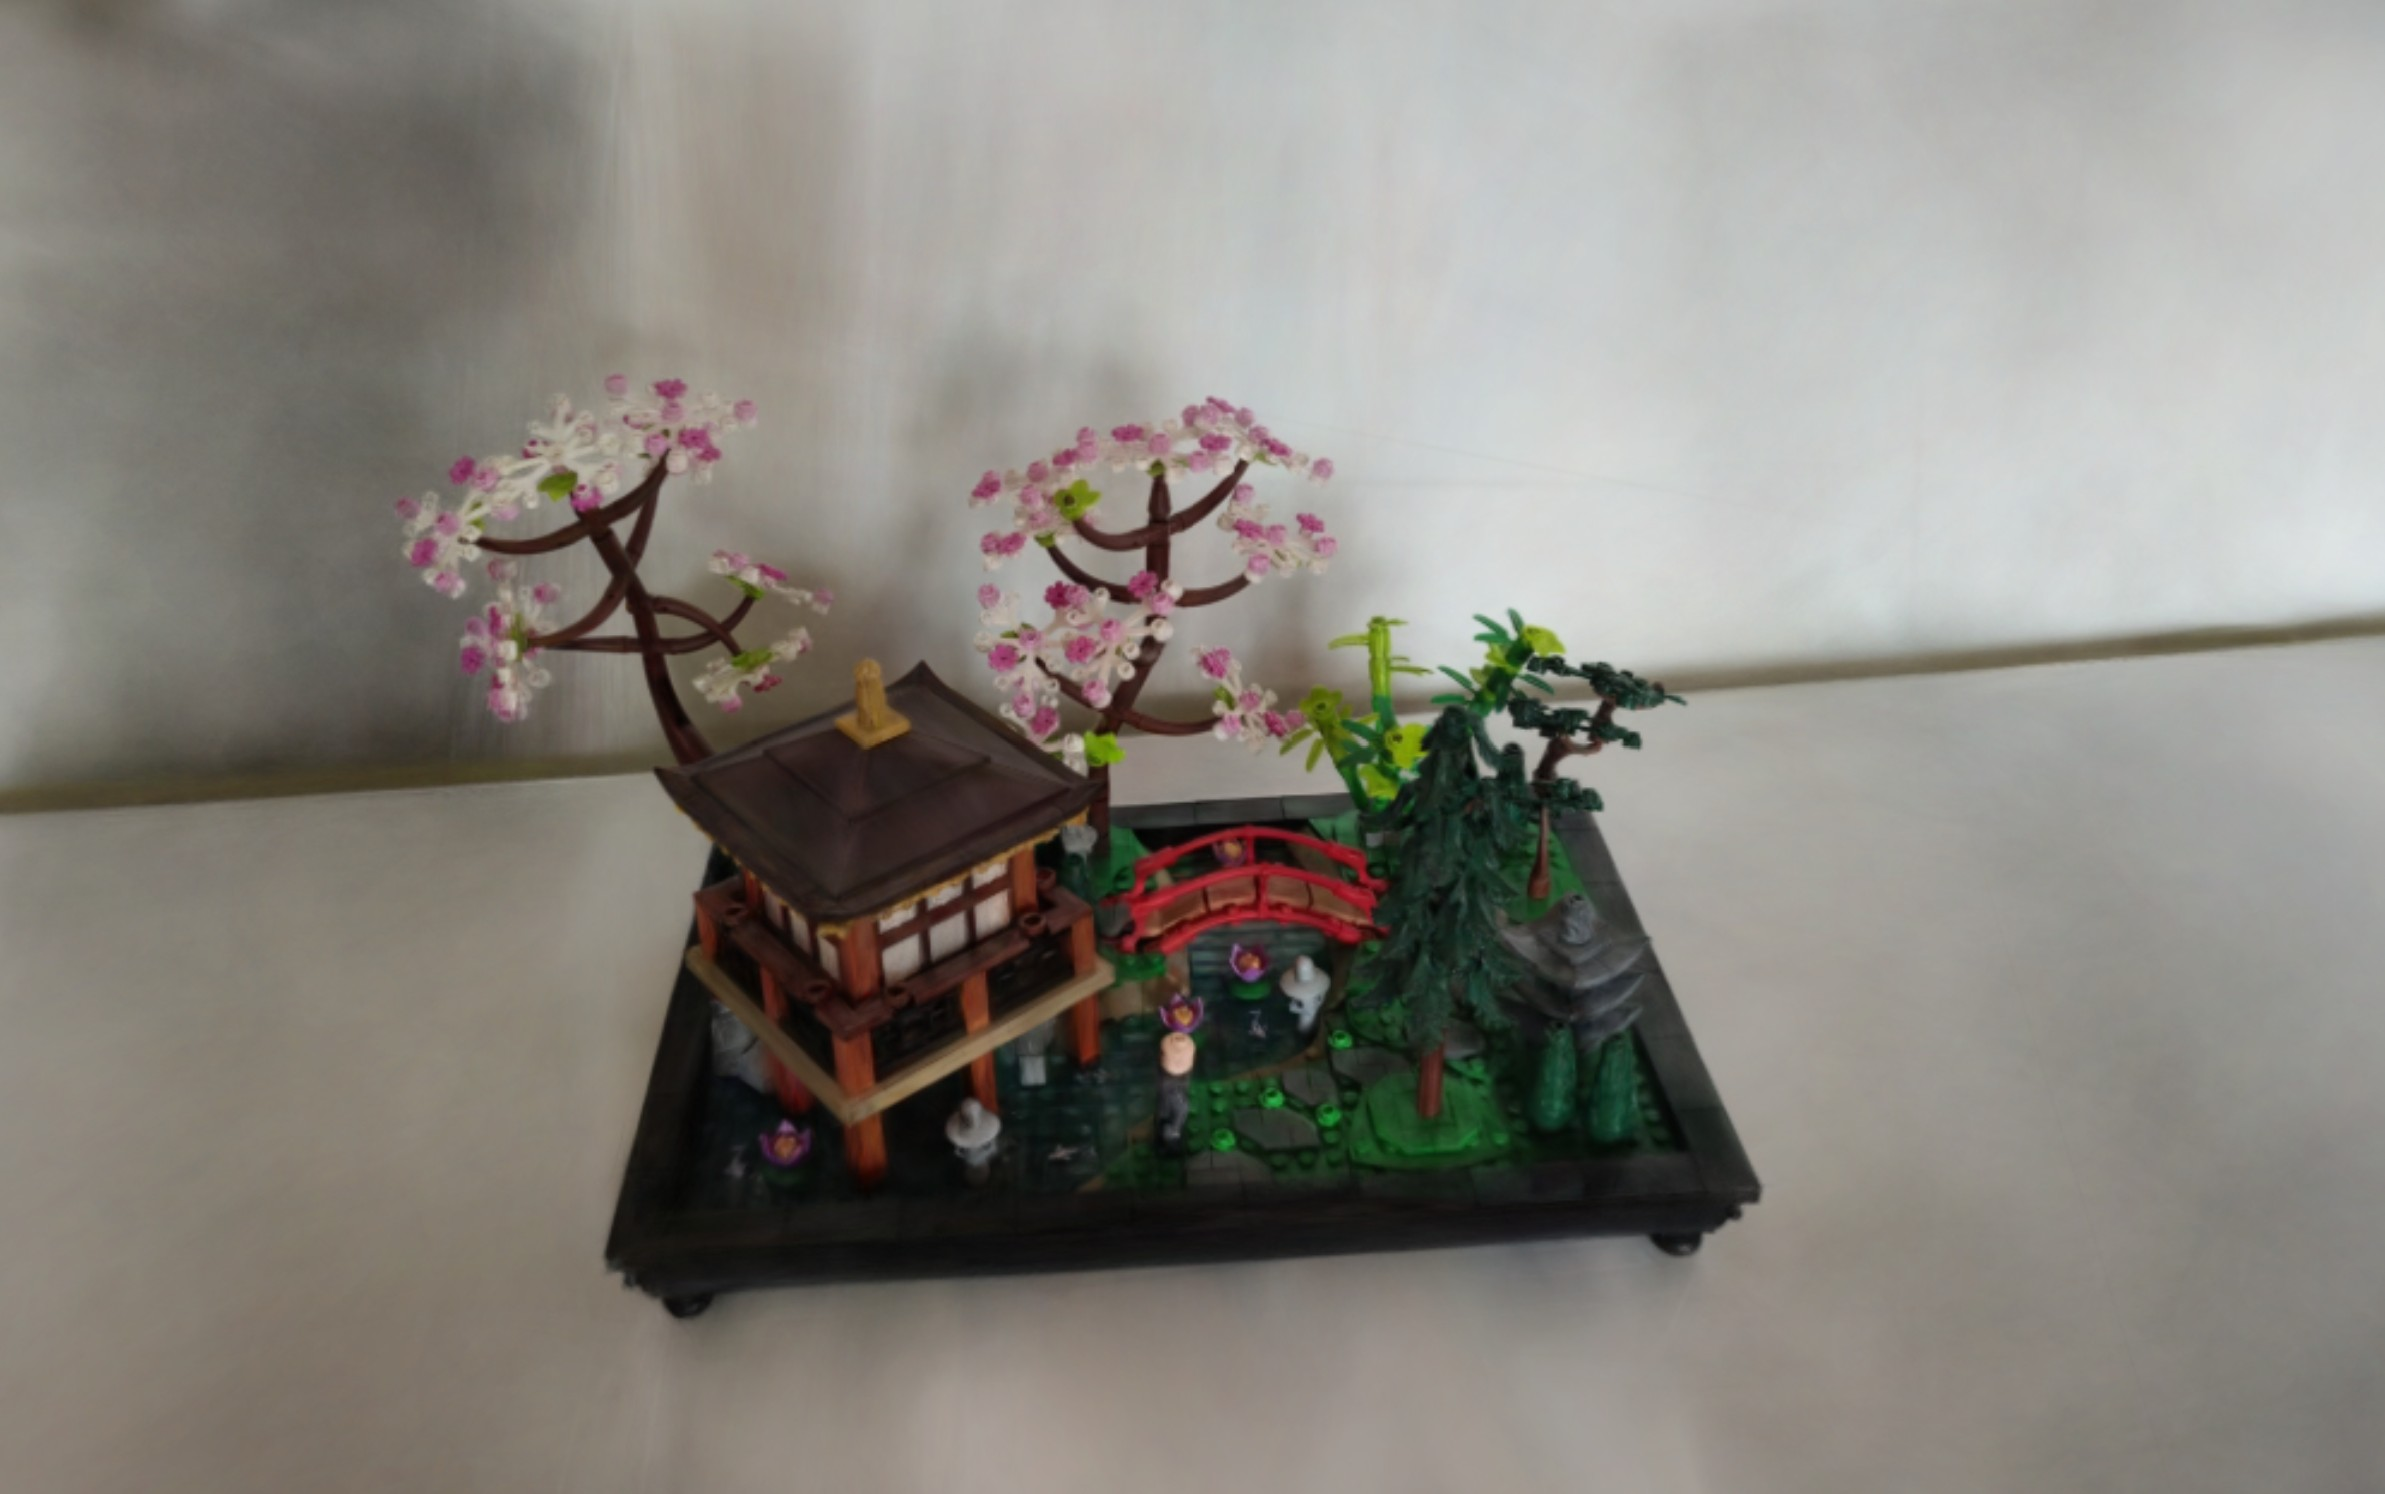
\includegraphics[width=\linewidth, height=2.3cm, trim={80 40 80 40}, clip]{images/benchmarks/lego_japanese_garden_taming_balanced.jpg}
		\caption{Balanced}
	\end{subfigure}
	\hfill
	\begin{subfigure}{0.32\textwidth}
		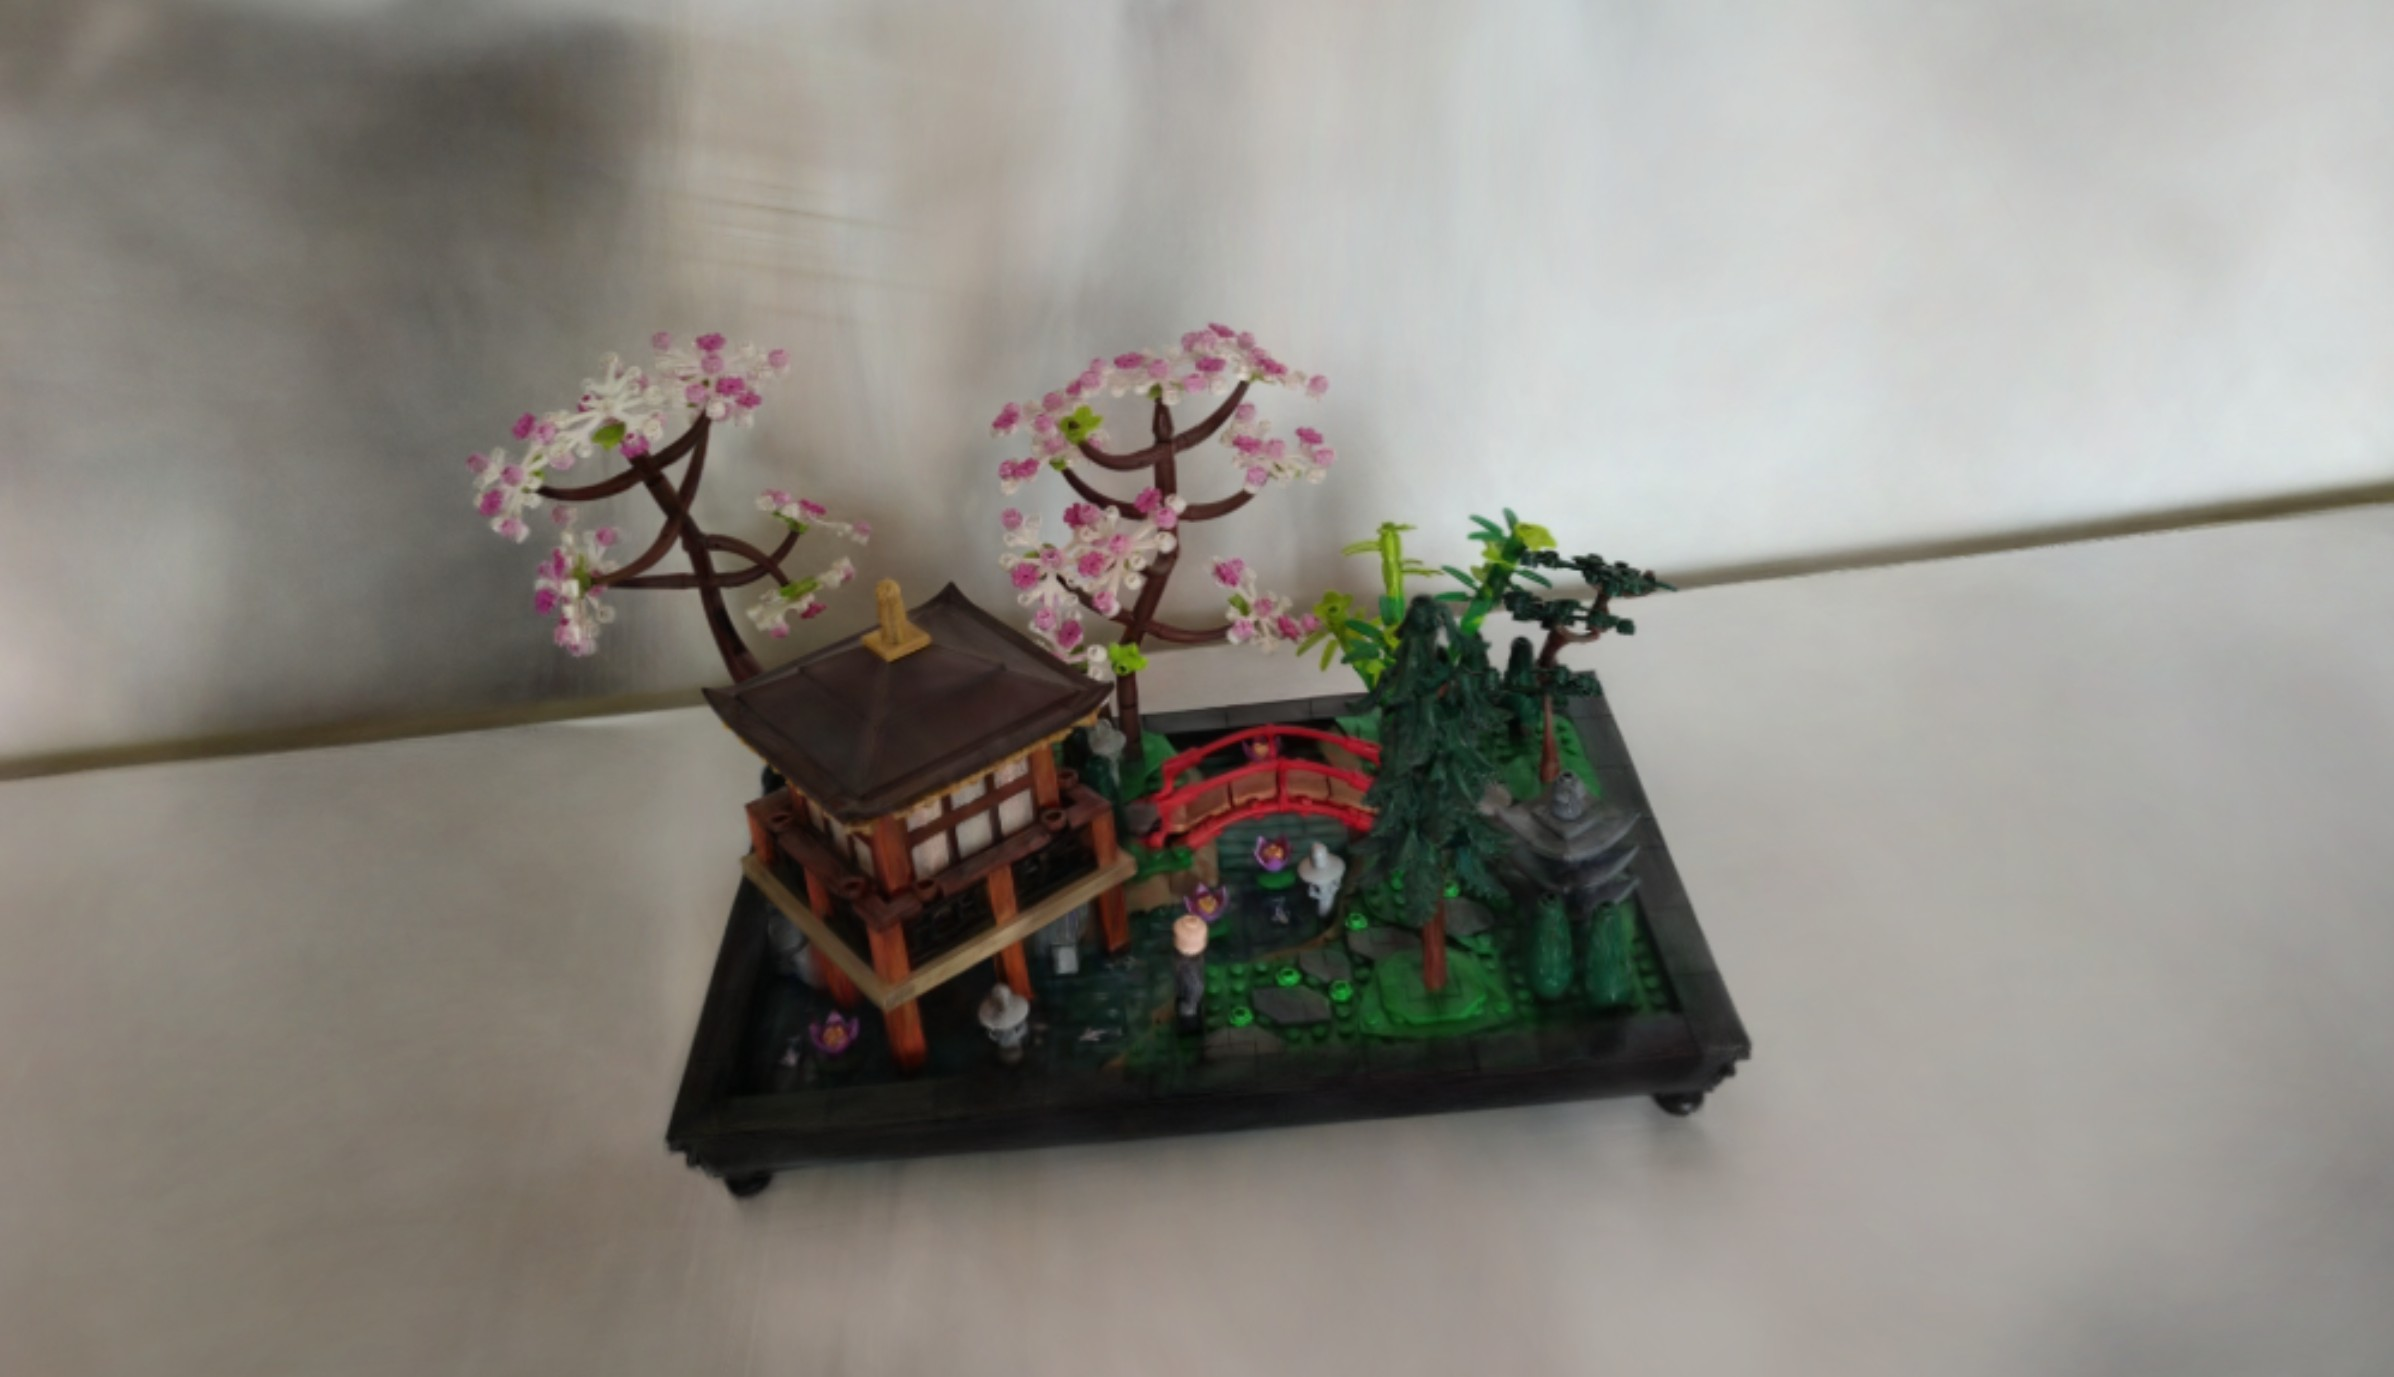
\includegraphics[width=\linewidth, height=2.3cm, trim={80 40 80 40}, clip]{images/benchmarks/lego_japanese_garden_taming_quality.jpg}
		\caption{Quality}
	\end{subfigure}
	\caption{Confronto visivo dei livelli di qualit\`a -- scena \textit{Lego Japanese Garden} (crop centrale).}
	\label{fig:lego_japanese_garden_quality_comparison}
\end{figure}

% ---------------------- IMMAGINI YELLOW PLANT ----------------------
\begin{figure}[H]
	\centering
	\begin{subfigure}{0.32\textwidth}
		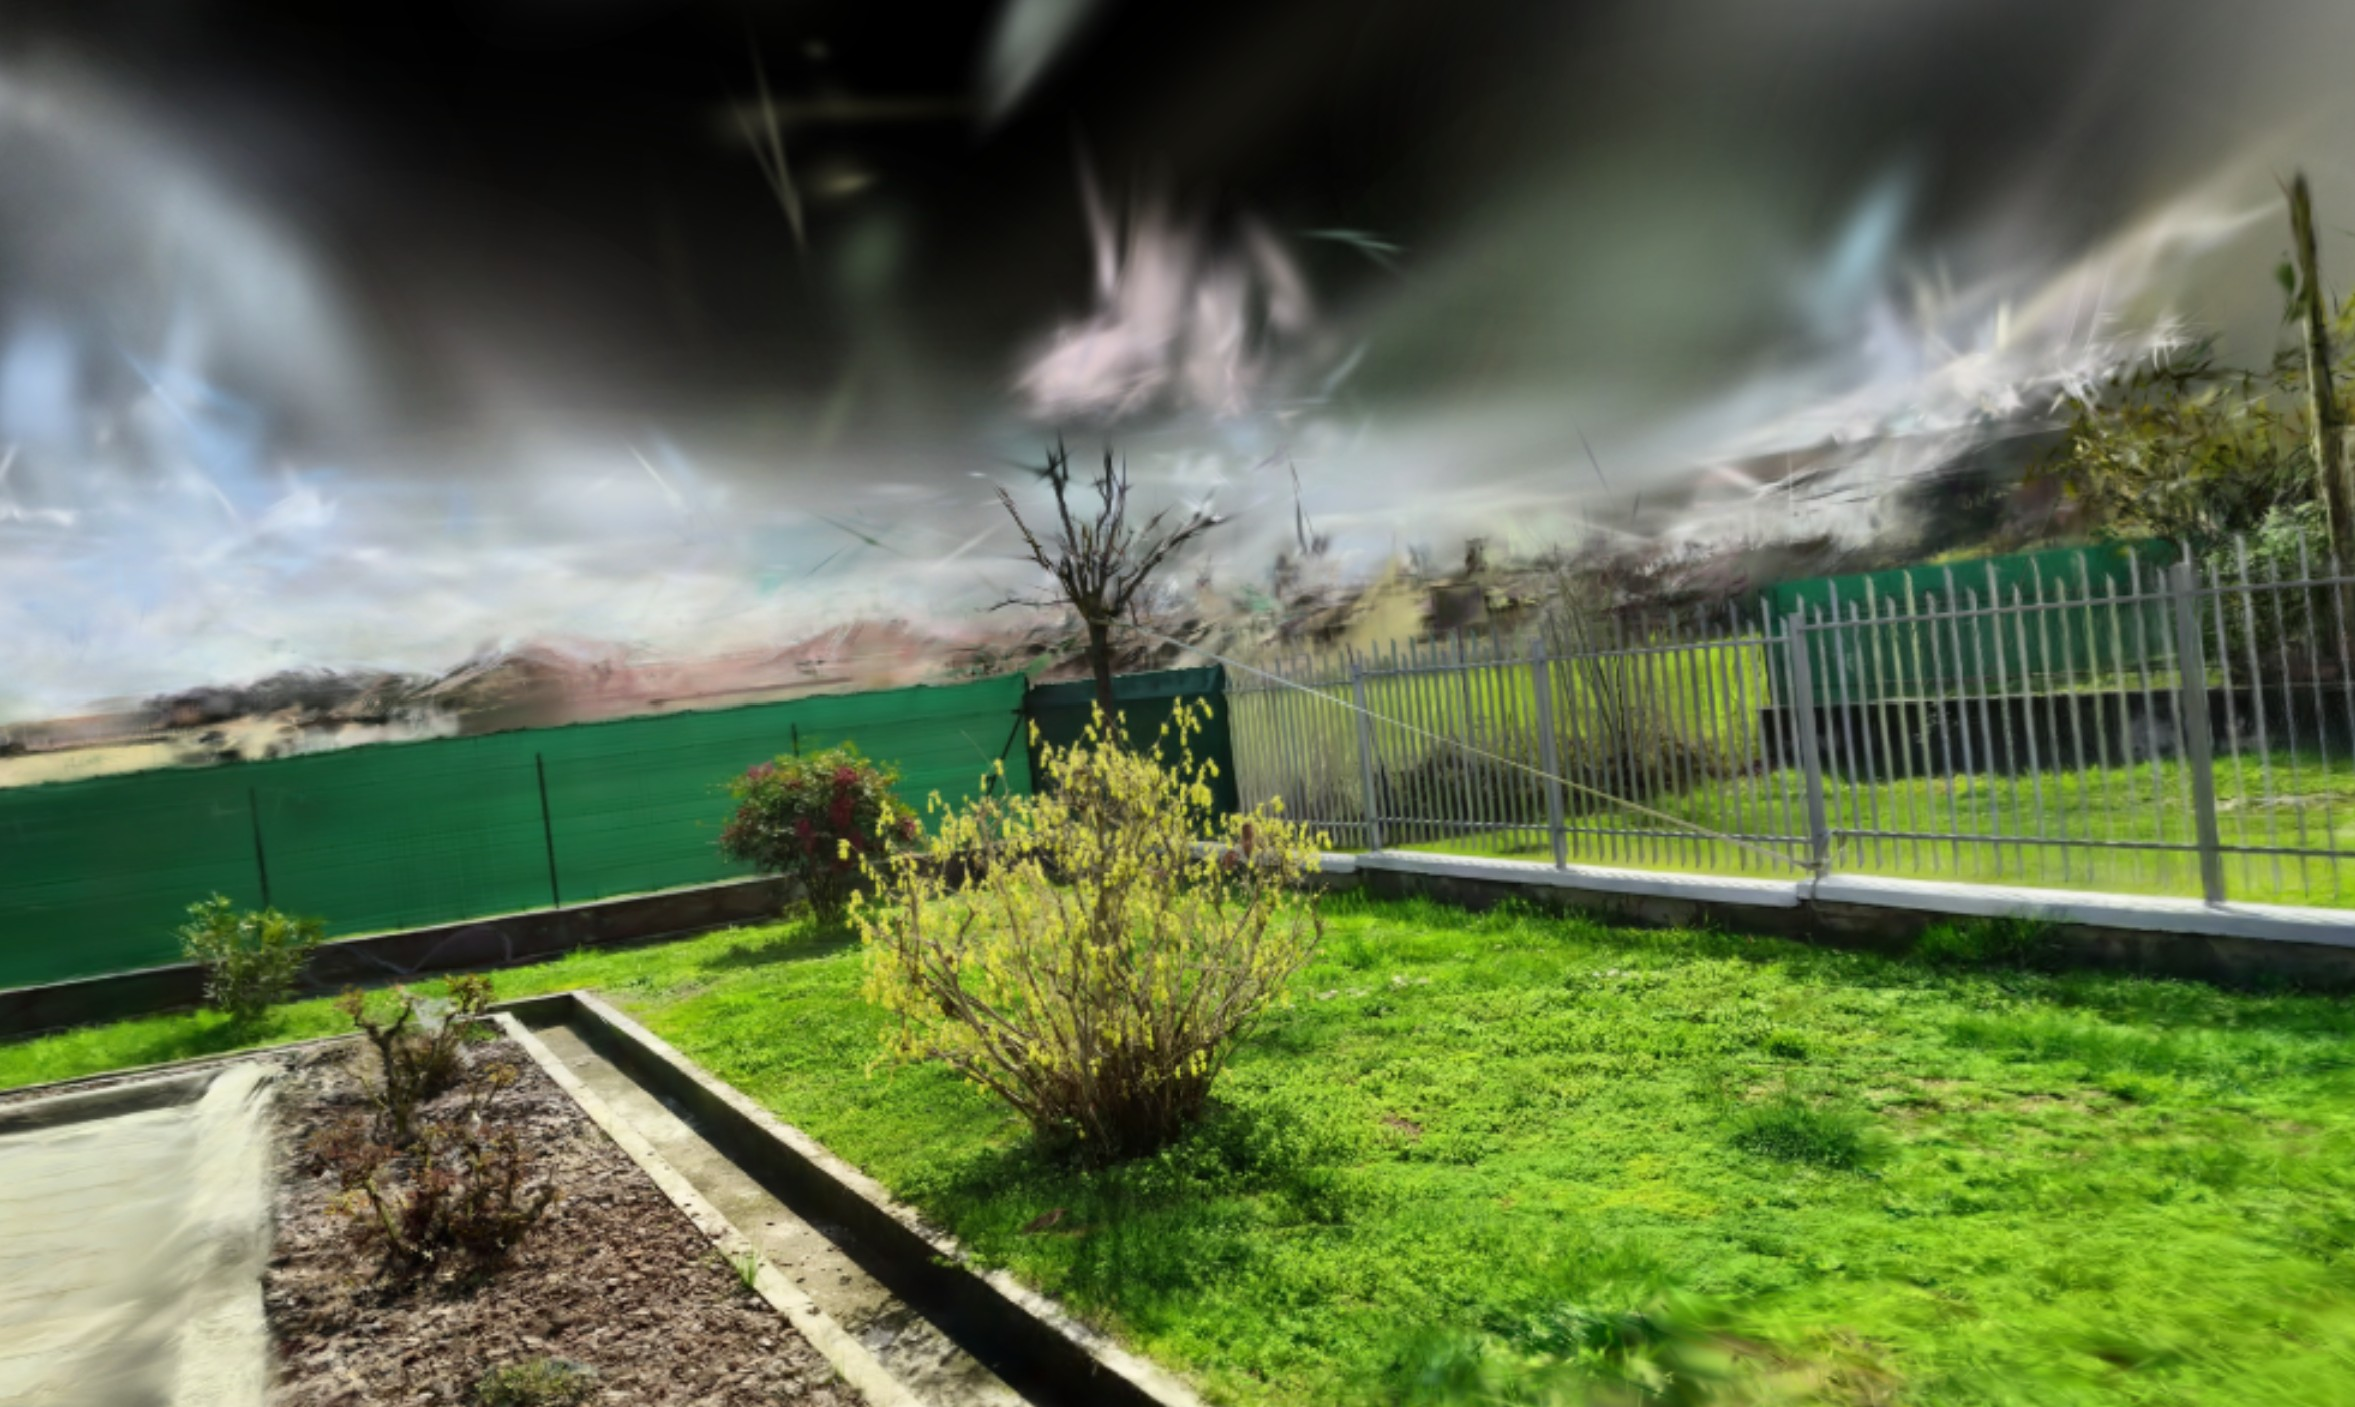
\includegraphics[width=\linewidth, height=2.3cm, trim={80 40 80 40}, clip]{images/benchmarks/yellow_plant_taming_fast.jpg}
		\caption{Fast}
	\end{subfigure}
	\hfill
	\begin{subfigure}{0.32\textwidth}
		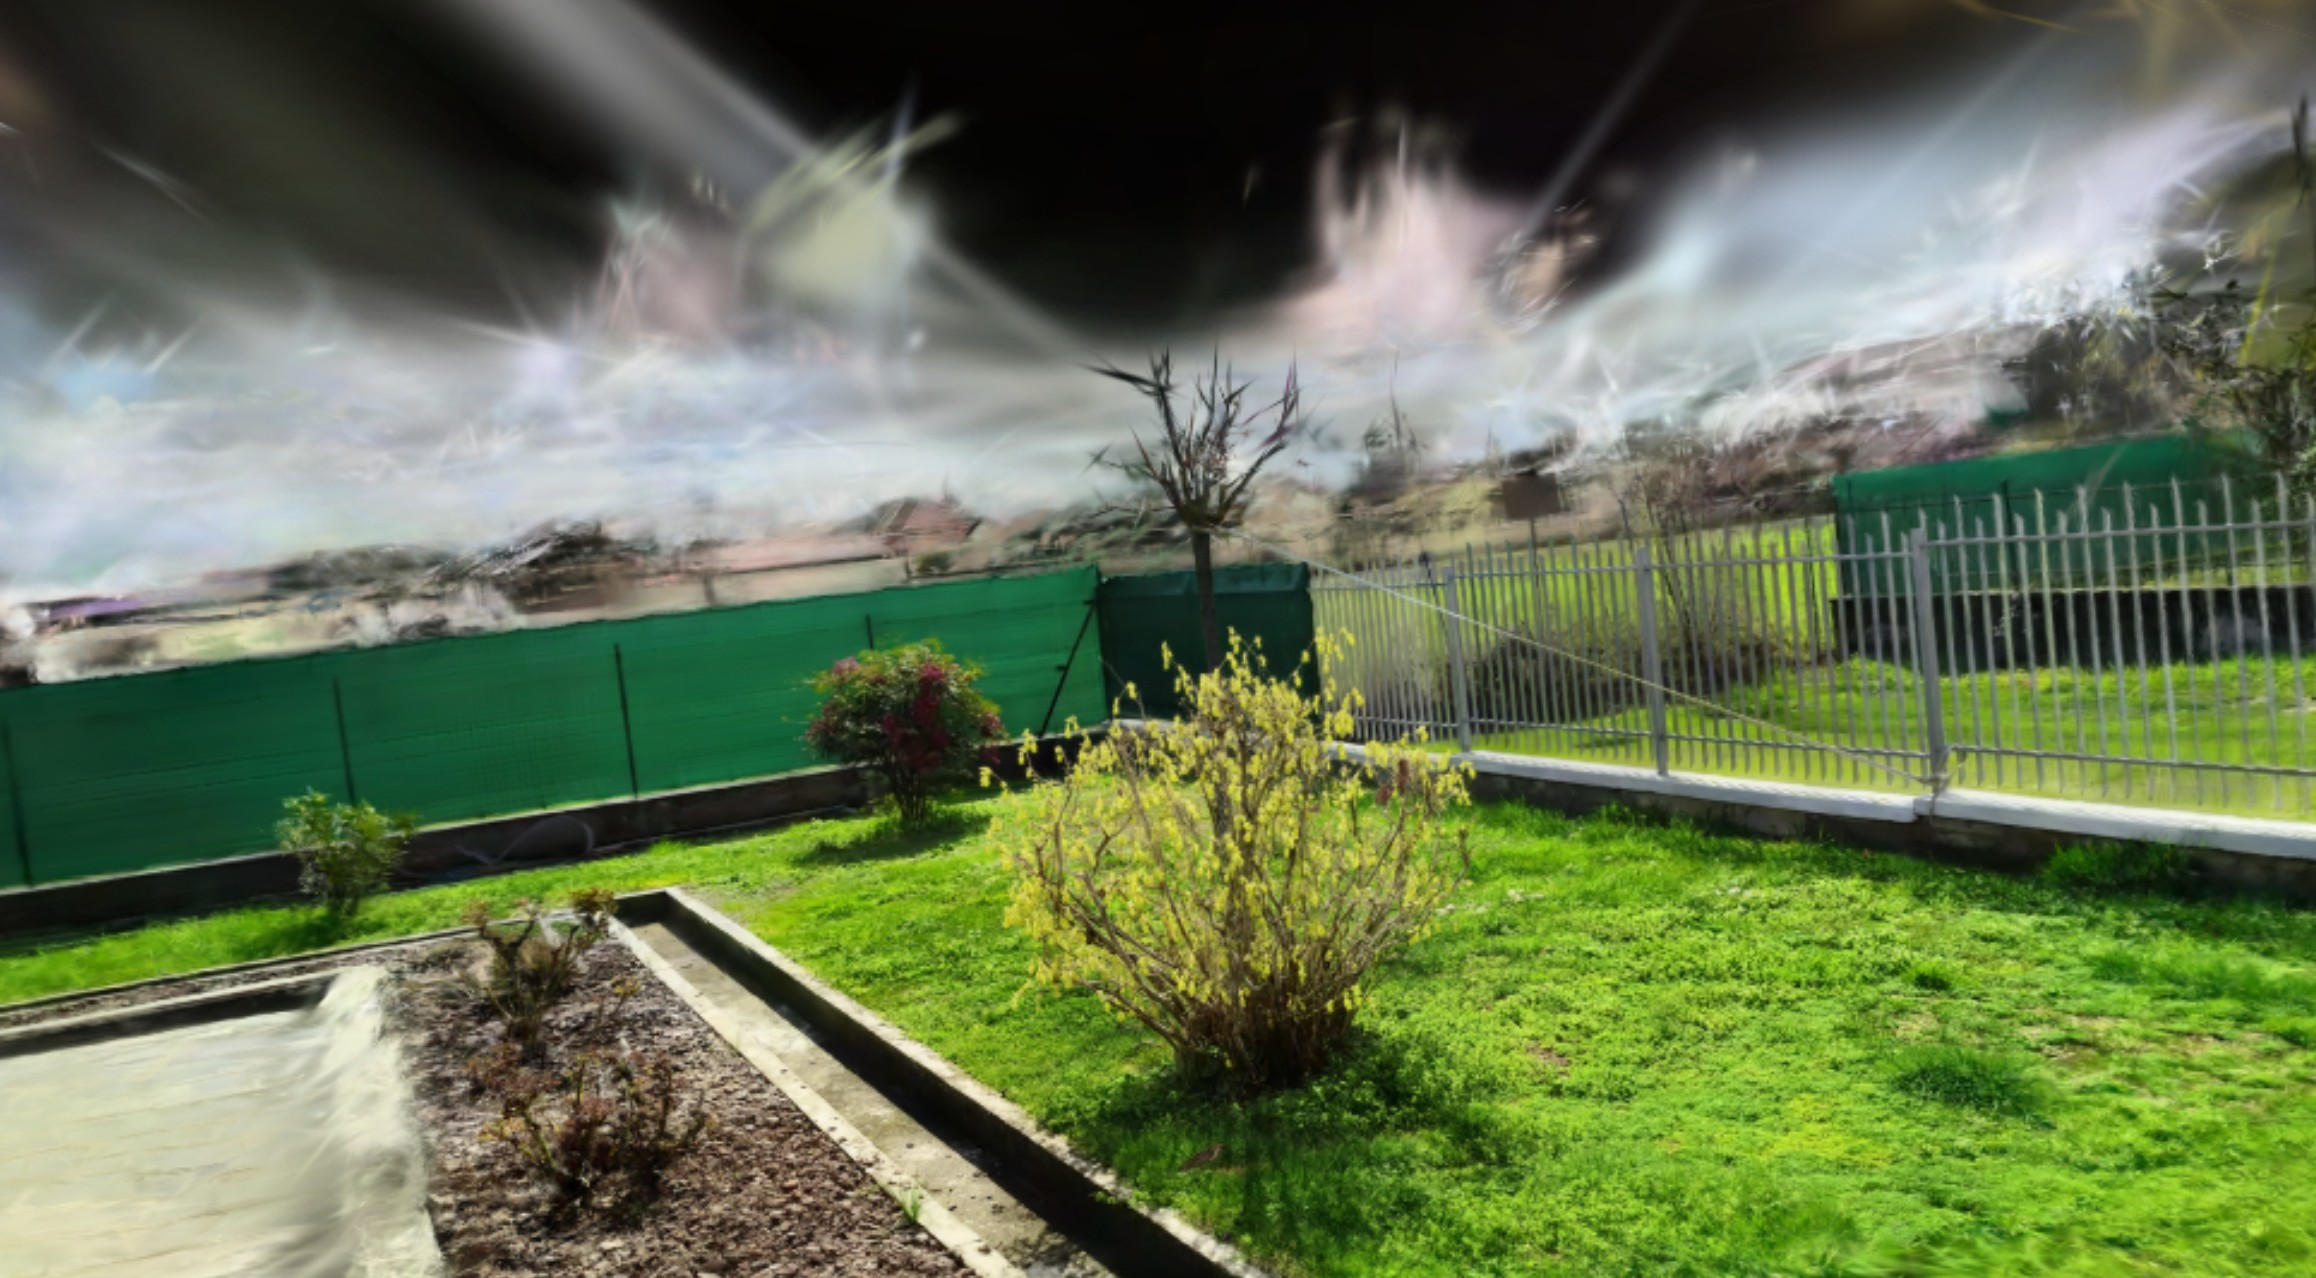
\includegraphics[width=\linewidth, height=2.3cm, trim={80 40 80 40}, clip]{images/benchmarks/yellow_plant_taming_balanced.jpg}
		\caption{Balanced}
	\end{subfigure}
	\hfill
	\begin{subfigure}{0.32\textwidth}
		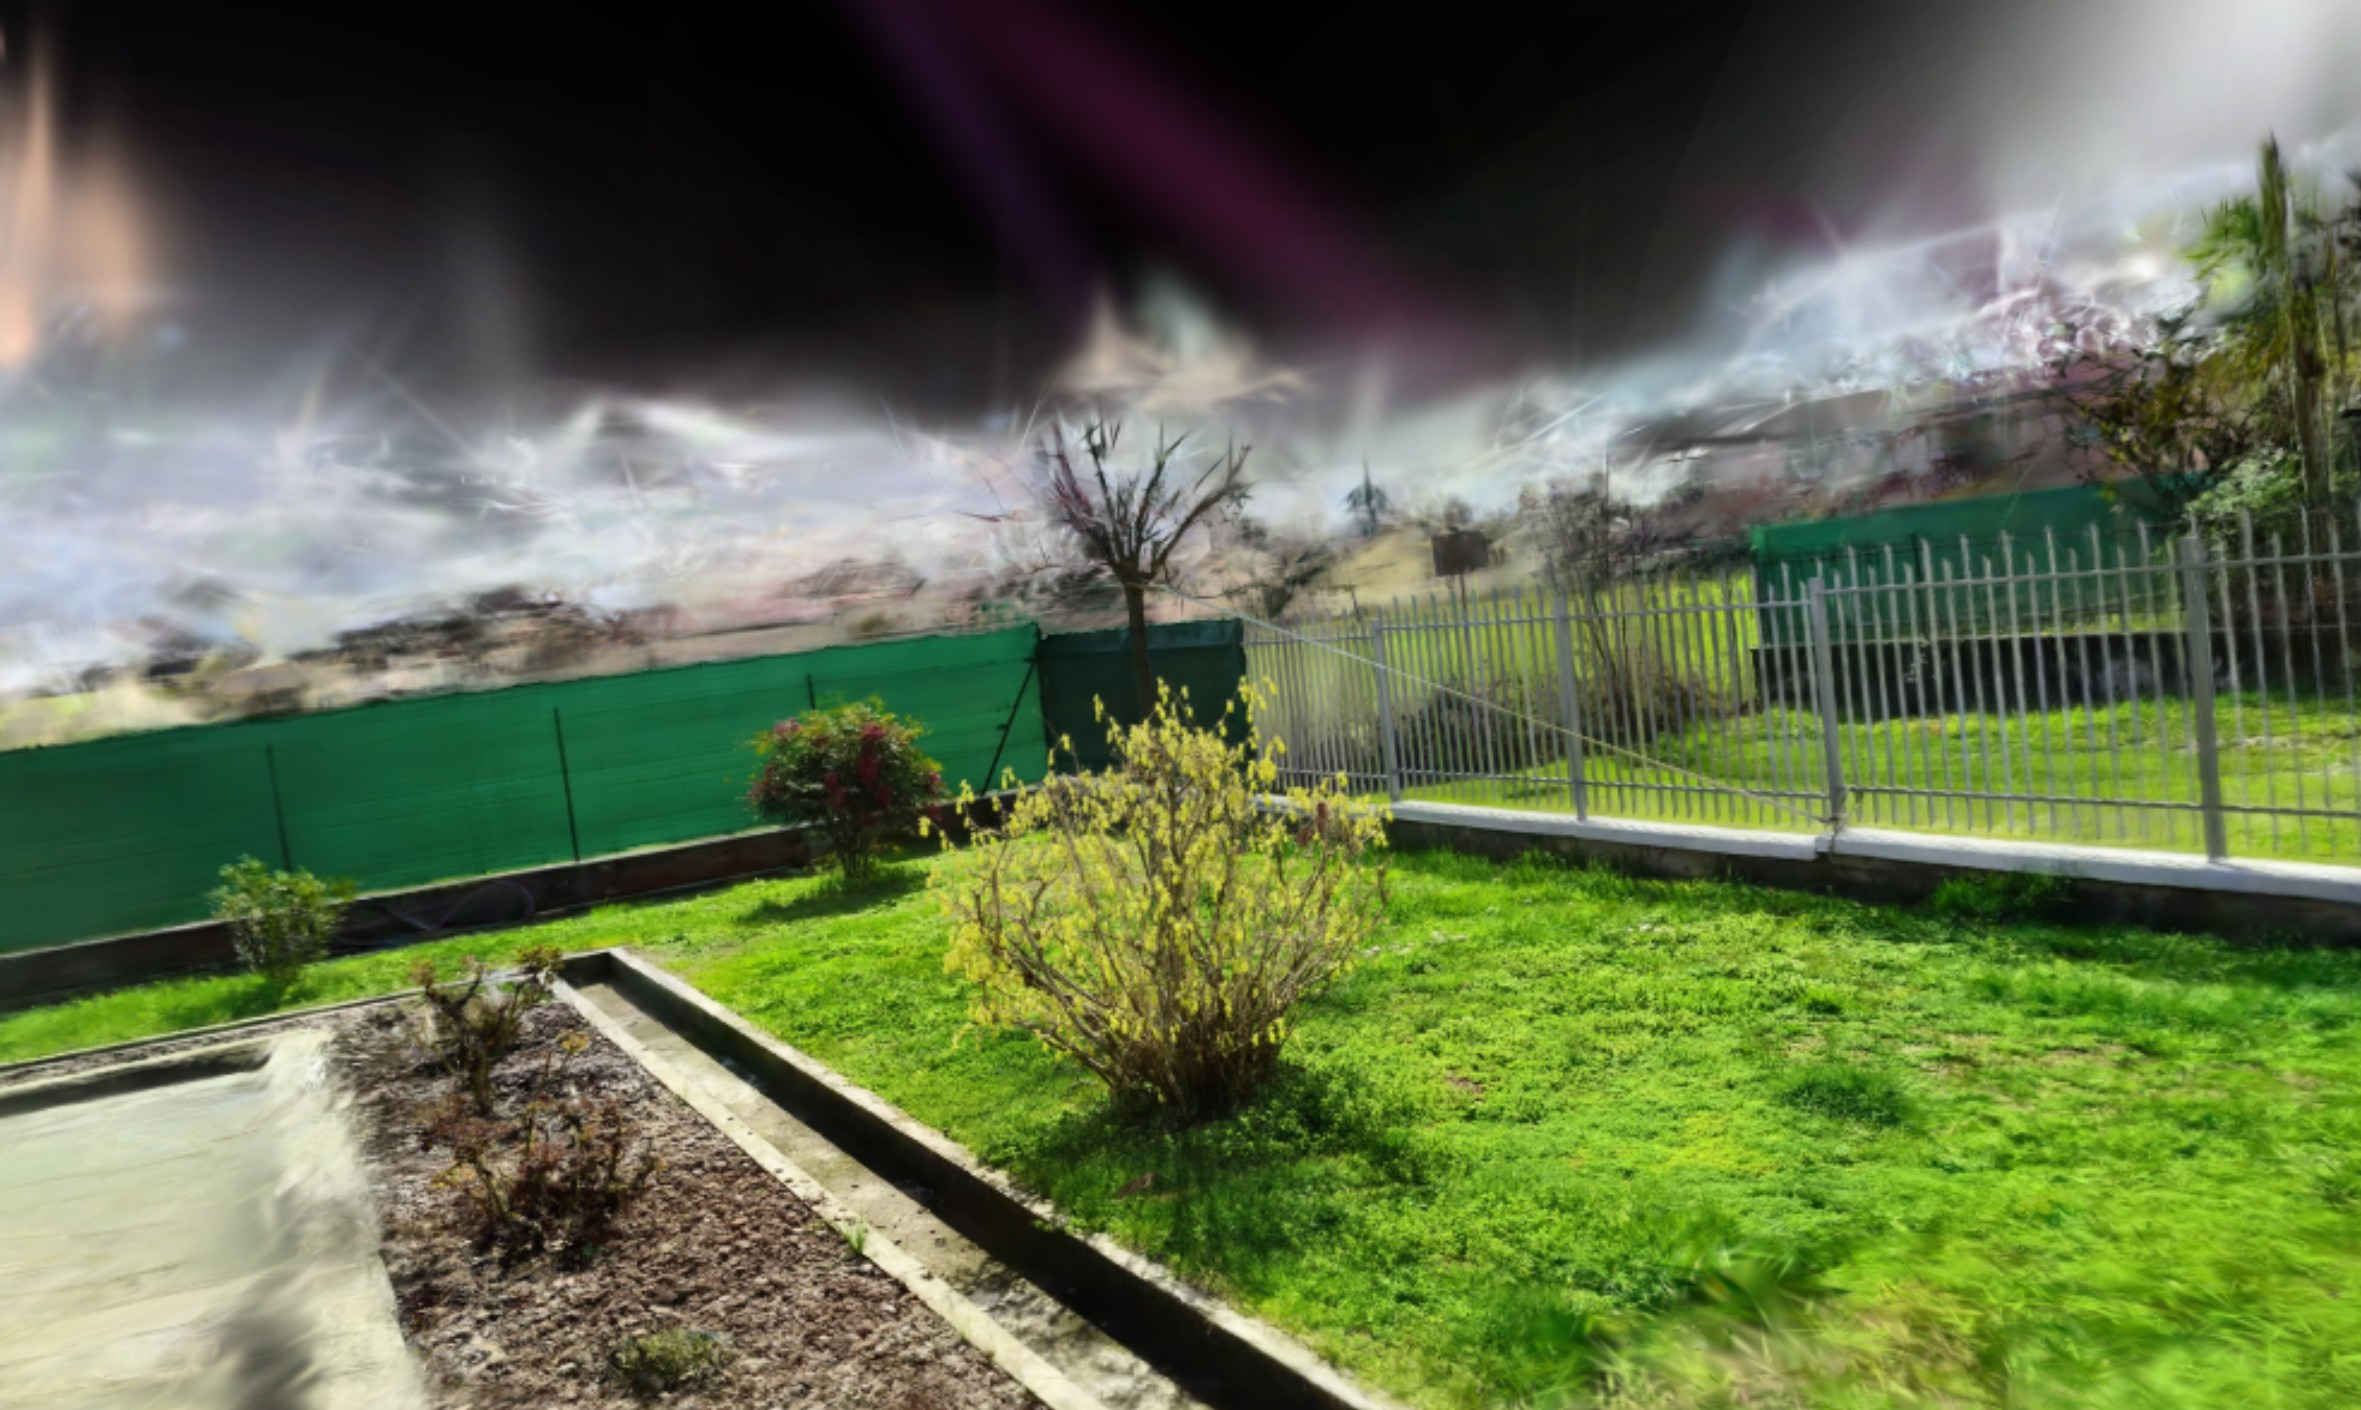
\includegraphics[width=\linewidth, height=2.3cm, trim={80 40 80 40}, clip]{images/benchmarks/yellow_plant_taming_quality.jpg}
		\caption{Quality}
	\end{subfigure}
	\caption{Confronto visivo dei livelli di qualit\`a -- scena \textit{Yellow Plant} (crop centrale).}
	\label{fig:yellow_plant_quality_comparison}
\end{figure}


\subsection{Benchmark 3: Latency Budget End-to-End (Balanced, 30k iterazioni)}
\label{subsec:latency_budget_inria}

\paragraph{Setup}
Tutti i test sono stati eseguiti con tutti gli algoritmi, preset \textbf{Balanced}, su una RTX 4080 16GB (WSL2).  
Il numero di iterazioni di training è fisso a \textbf{30\,000} per tutte le scene.  
Le metriche PSNR/SSIM/LPIPS sono calcolate in un job asincrono e non influiscono sul \emph{time-to-preview}.

% --- RIEPILOGO PER SCENA ---
\begin{table}[H]
	\centering
	\caption{Riepilogo end-to-end per scena - INRIA}
	\label{tab:inria_summary_per_scene}
	\footnotesize
	\begin{tabularx}{\textwidth}{@{} l L L L L @{}}
		\toprule
		\textbf{Scena} & \textbf{Tempo Totale (s)} & \textbf{\#Frame} & \textbf{Punti COLMAP} & \textbf{Gauss. finali} \\
		\midrule
		S1 — \textit{Master of Puppets} &
		917 &
		189 &
		61\,014 &
		324\,662 \\
		S2 — \textit{Lego Display Window} &
		866 &
		234 &
		30\,304 &
		470\,058 \\
		S3 — \textit{Yellow Plant} &
		1416 &
		202 &
		120\,521 &
		1\,409\,058 \\
		\bottomrule
	\end{tabularx}
\end{table}


% ---------- S1: Master of Puppets ----------
\begin{figure}[H]
	\centering
	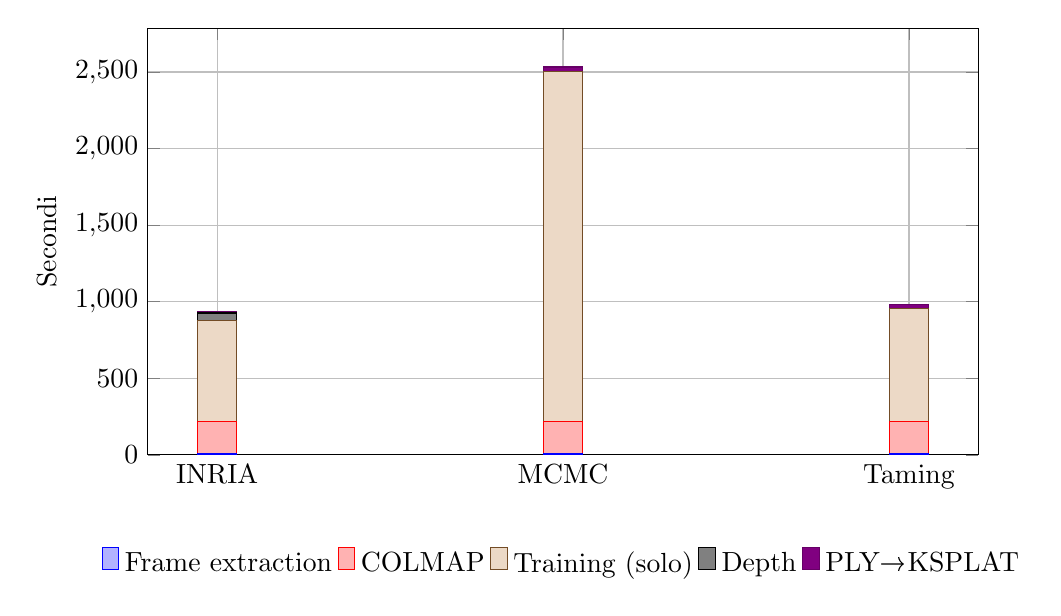
\begin{tikzpicture}
		\begin{axis}[
			ybar stacked, bar width=14pt,
			ylabel={Secondi},
			symbolic x coords={INRIA,MCMC,Taming},
			xtick=data,
			ymin=0, height=7cm, width=\linewidth,
			grid=both,
			legend columns=5, legend cell align=left,
			legend style={at={(0.5,-0.2)},anchor=north,draw=none}
			]
			% S1 tempi per algoritmo
			% Frame extraction (uguale per tutti)
			\addplot coordinates {(INRIA,8.14) (MCMC,8.14) (Taming,8.14)}; \addlegendentry{Frame extraction}
			% COLMAP (uguale per tutti)
			\addplot coordinates {(INRIA,209.46) (MCMC,209.46) (Taming,209.46)}; \addlegendentry{COLMAP}
			% Training (solo)
			\addplot coordinates {(INRIA,661.82) (MCMC,2285.02) (Taming,738.24)}; \addlegendentry{Training (solo)}
			% Depth (solo INRIA)
			\addplot coordinates {(INRIA,46.65) (MCMC,0) (Taming,0)}; \addlegendentry{Depth}
			% PLY→KSPLAT
			\addplot coordinates {(INRIA,8.24) (MCMC,29.98) (Taming,27.76)}; \addlegendentry{PLY→KSPLAT}
		\end{axis}
	\end{tikzpicture}
	\caption{Latency budget per algoritmo — \emph{S1: Master of Puppets} (Balanced, 30k).}
	\label{fig:s1_algos}
\end{figure}

% ---------- S2: Lego Display Window ----------
\begin{figure}[H]
	\centering
	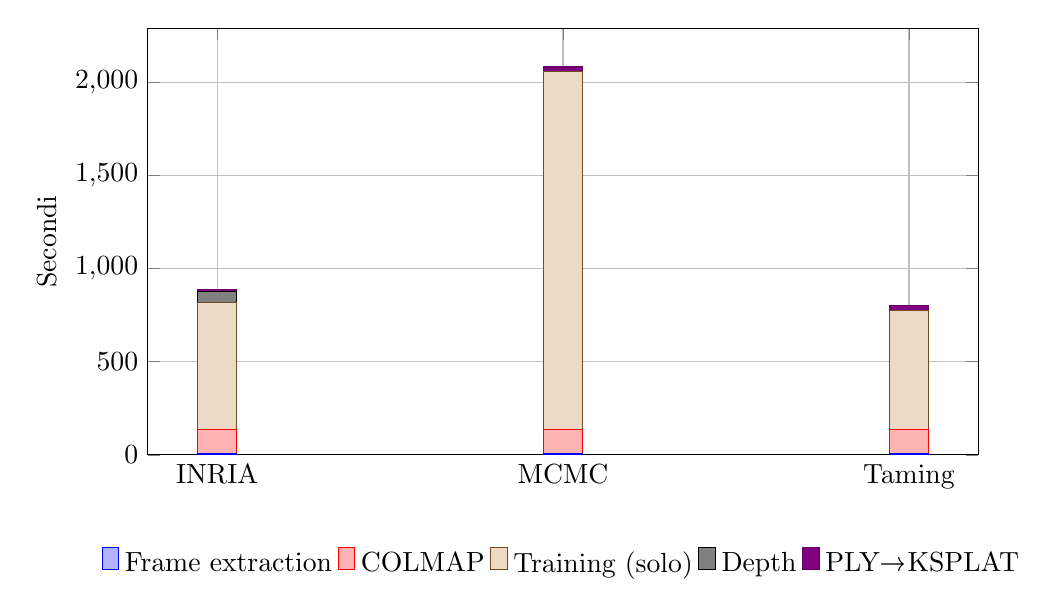
\begin{tikzpicture}
		\begin{axis}[
			ybar stacked, bar width=14pt,
			ylabel={Secondi},
			symbolic x coords={INRIA,MCMC,Taming},
			xtick=data,
			ymin=0, height=7cm, width=\linewidth,
			grid=both,
			legend columns=5, legend cell align=left,
			legend style={at={(0.5,-0.2)},anchor=north,draw=none}
			]
			% Frame extraction (uguale)
			\addplot coordinates {(INRIA,8.14) (MCMC,8.14) (Taming,8.14)}; \addlegendentry{Frame extraction}
			% COLMAP (uguale)
			\addplot coordinates {(INRIA,127.63) (MCMC,127.63) (Taming,127.63)}; \addlegendentry{COLMAP}
			% Training (solo)
			\addplot coordinates {(INRIA,683.23) (MCMC,1919.04) (Taming,637.85)}; \addlegendentry{Training (solo)}
			% Depth (solo INRIA)
			\addplot coordinates {(INRIA,55.73) (MCMC,0) (Taming,0)}; \addlegendentry{Depth}
			% PLY→KSPLAT
			\addplot coordinates {(INRIA,13.95) (MCMC,26.11) (Taming,28.19)}; \addlegendentry{PLY→KSPLAT}
		\end{axis}
	\end{tikzpicture}
	\caption{Latency budget per algoritmo — \emph{S2: Lego Display Window} (Balanced, 30k).}
	\label{fig:s2_algos}
\end{figure}

% ---------- S3: Yellow Plant ----------
\begin{figure}[H]
	\centering
	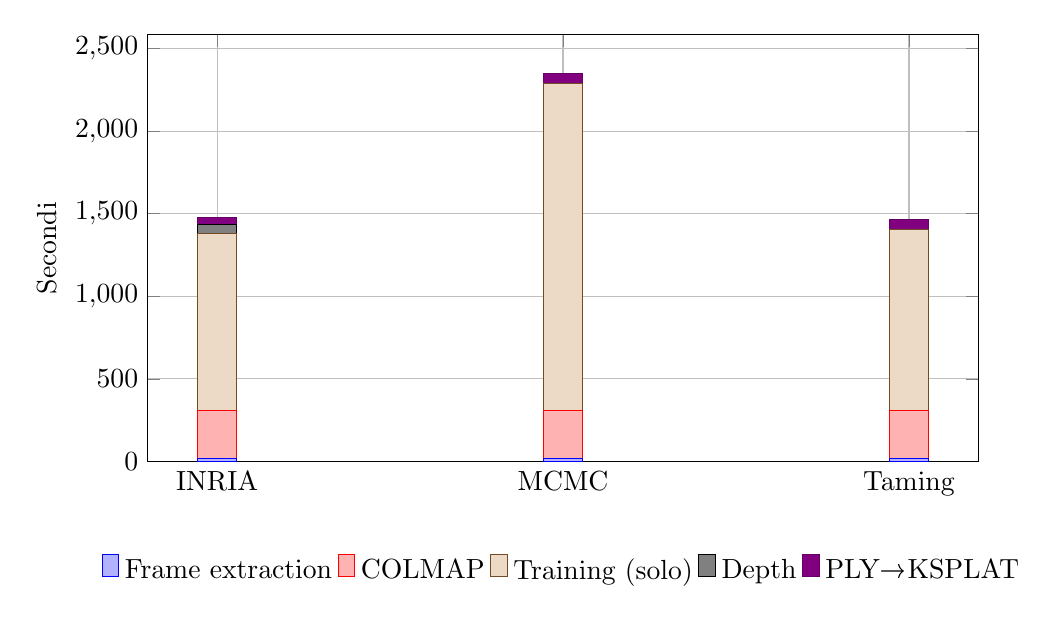
\begin{tikzpicture}
		\begin{axis}[
			ybar stacked, bar width=14pt,
			ylabel={Secondi},
			symbolic x coords={INRIA,MCMC,Taming},
			xtick=data,
			ymin=0, height=7cm, width=\linewidth,
			grid=both,
			legend columns=5, legend cell align=left,
			legend style={at={(0.5,-0.2)},anchor=north,draw=none}
			]
			% Frame extraction (uguale)
			\addplot coordinates {(INRIA,17.03) (MCMC,17.03) (Taming,17.03)}; \addlegendentry{Frame extraction}
			% COLMAP (uguale)
			\addplot coordinates {(INRIA,291.85) (MCMC,291.85) (Taming,291.85)}; \addlegendentry{COLMAP}
			% Training (solo)
			\addplot coordinates {(INRIA,1072.53) (MCMC,1976.65) (Taming,1092.70)}; \addlegendentry{Training (solo)}
			% Depth (solo INRIA)
			\addplot coordinates {(INRIA,52.24) (MCMC,0) (Taming,0)}; \addlegendentry{Depth}
			% PLY→KSPLAT
			\addplot coordinates {(INRIA,45.15) (MCMC,62.77) (Taming,61.99)}; \addlegendentry{PLY→KSPLAT}
		\end{axis}
	\end{tikzpicture}
	\caption{Latency budget per algoritmo — \emph{S3: Yellow Plant} (Balanced, 30k).}
	\label{fig:s3_algos}
\end{figure}



\begin{figure}[H]
	\centering
	% --- Pannello 1: ratio KSPLAT/PLY ---
	\begin{minipage}{0.47\linewidth}
		\centering
		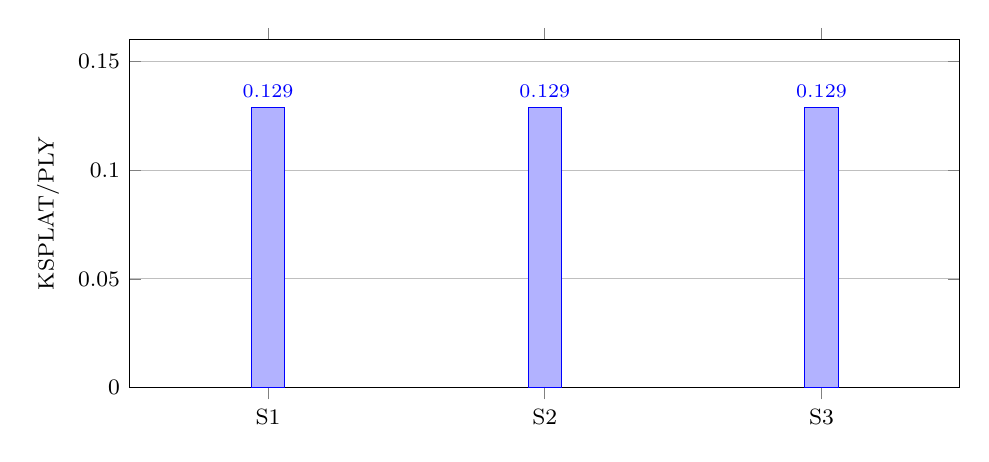
\begin{tikzpicture}
			\begin{axis}[
				ybar, bar width=12pt,
				ylabel={KSPLAT/PLY},
				ylabel style={font=\footnotesize},
				symbolic x coords={S1,S2,S3},
				xtick=data,
				ymin=0, ymax=0.16,
				ymajorgrids,
				height=6cm, width=\linewidth,
				enlarge x limits=0.25,
				tick label style={font=\footnotesize},
				y tick label style={/pgf/number format/fixed,/pgf/number format/precision=3},
				nodes near coords,
				nodes near coords align={vertical},
				every node near coord/.append style={font=\scriptsize, /pgf/number format/precision=3}
				]
				\addplot coordinates {(S1,0.129) (S2,0.129) (S3,0.129)};
			\end{axis}
		\end{tikzpicture}
	\end{minipage}
	\hfill
	% --- Pannello 2: tempo per MB ---
	\begin{minipage}{0.47\linewidth}
		\centering
		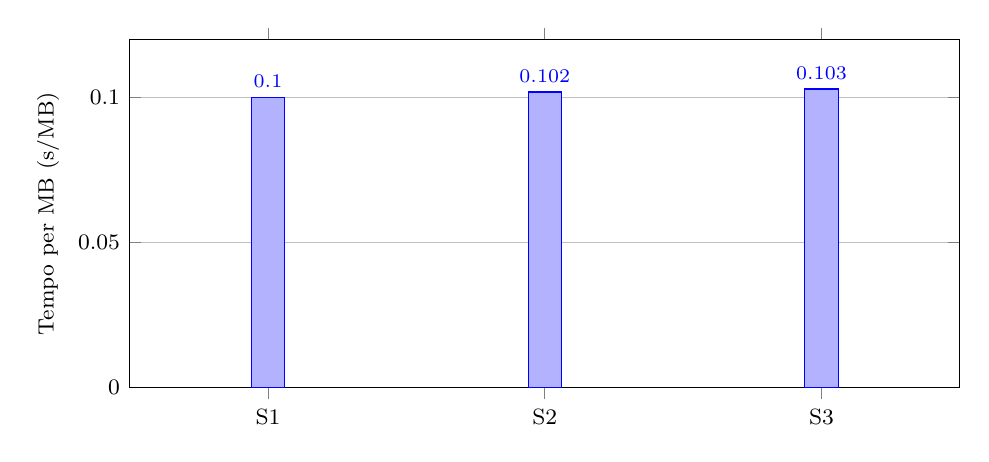
\begin{tikzpicture}
			\begin{axis}[
				ybar, bar width=12pt,
				ylabel={Tempo per MB (s/MB)},
				ylabel style={font=\footnotesize},
				symbolic x coords={S1,S2,S3},
				xtick=data,
				ymin=0, ymax=0.12,
				ymajorgrids,
				height=6cm, width=\linewidth,
				enlarge x limits=0.25,
				tick label style={font=\footnotesize},
				y tick label style={/pgf/number format/fixed,/pgf/number format/precision=3},
				nodes near coords,
				nodes near coords align={vertical},
				every node near coord/.append style={font=\scriptsize, /pgf/number format/precision=3}
				]
				\addplot coordinates {(S1,0.100) (S2,0.102) (S3,0.103)};
			\end{axis}
		\end{tikzpicture}
	\end{minipage}
	
	\caption{Efficienza conversione PLY$\rightarrow$KSPLAT: rapporto di compressione e costo computazionale.}
	\label{fig:ply_splat_efficiency_minipage}
\end{figure}

\begin{figure}[H]
	\centering
	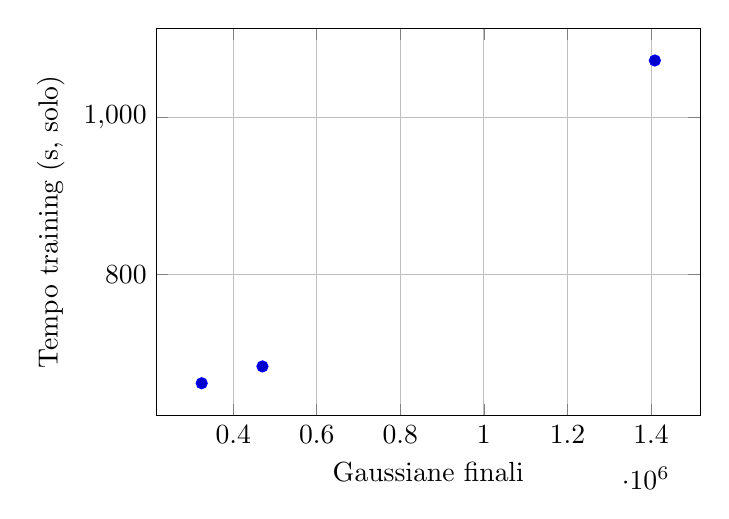
\begin{tikzpicture}
		\begin{axis}[
			xlabel={Gaussiane finali}, ylabel={Tempo training (s, solo)},
			xmajorgrids, ymajorgrids, height=6.5cm, width=0.7\linewidth
			]
			\addplot+[only marks, mark=*] coordinates {
				(324662,661.82)
				(470058,683.23)
				(1409058,1072.53)
			};
		\end{axis}
	\end{tikzpicture}
	\caption{Durata del training (parte ottimizzazione) in funzione delle gaussiane finali.}
	\label{fig:train_vs_gauss}
\end{figure}

\paragraph{Osservazioni}
Dall’analisi del \emph{latency budget} (Tab.~\ref{tab:inria_budget_all} e Fig.~\ref{fig:stacked_time_per_phase}) emerge come:
\begin{itemize}
	\item La fase di \textbf{training} sia nettamente la più onerosa in termini di tempo, assorbendo dal 72\% al 79\% del \emph{time-to-preview}, seguita dalla \textbf{ricostruzione COLMAP} (15–23\%).
	\item La \textbf{depth regularization} incide in media per circa il 22–25\% del tempo di training, con valori piuttosto stabili tra le scene.
	\item La \textbf{frame extraction} e la conversione \textbf{PLY$\rightarrow$KSPLAT} hanno un peso marginale, inferiore al 4\% complessivo, e costi computazionali per MB molto simili tra le scene (Fig.~\ref{fig:ply_ksplat_efficiency_minipage}).
	\item Il rapporto di compressione PLY/KSPLAT è costante (0.129) grazie a una pipeline di conversione stabile e indipendente dalla complessità della scena.
	\item Come mostra Fig.~\ref{fig:train_vs_gauss}, il tempo di training cresce con il numero di gaussiane finali, ma non in modo perfettamente lineare: scene con distribuzioni spaziali più complesse o ricche di dettagli (es. \emph{Yellow Plant}) possono richiedere tempi superiori a parità di incremento percentuale di gaussiane.
\end{itemize}

Questi dati, pur riferendosi al solo caso \emph{INRIA Balanced} con 30\,000 iterazioni, costituiscono una base per confronti futuri con altre configurazioni o algoritmi (MCMC, Taming) mantenendo costante la metodologia di misura.
